\documentclass[../main.tex]{subfiles}

\begin{document}

\selectlanguage{english}
\chapter{Résumé étendu en français}

\section{Contexte et Motivation}\label{sec:cont-et-motiv}

L'évolution de la computation dans les dernières deux décades est indéniable.
Dispositifs avec la même puissance des ordinateurs qui ont possibilité l'humanité à toucher le sol lunaire dans la décade de $1970$ sont aujourd'hui à la distance d'une main.

Cette évolution a proportionné l'utilisation de la commande prédictive~\cite{GarciaEtAl1989}, en anglais
connue comme \mpclong{} ou \mpcshort, en problèmes avec échelles de temps réduites, quelquefois en temps-réel~\cite{BesselmannEtAl2008}, et en utilisant dispositifs plus petits qu'une pièce~\cite{BanguraMahony2014}.

Aussi comme conséquence la \mpc{} est envisagée pour contrôler systèmes dans une myriade d'applications avec l'échelle de villes, comme les réseaux de distribution d'eau~\cite{ZhangEtAl2021}, en anglais
\wdns, et de chaleur~\cite{TaylorEtAl2021}, en anglais \dhns.
Ça présente l'insertion de la \mpc{} dans les systèmes cyber-physiques, en anglais \cps{}, où ordinateurs et machines sont étroitement couplées.

Cependant, pour quelques systèmes de grande échelles, le calcul peut encore être coûteuse, nécessitant de stratégies, comme diviser le calcul en plusieurs dispositfs, à fin de faciliter la computation.
Comme on verra cette stratégie est appelée commande prédictive distribuée, ou \dmpc{}, et cela vient en differents moutures.

Néanmoins, pas trop d'études ont été faites pour la sécurité des stratégies \dmpc{}, quand les agents ne communiquent honnêtement.
Ce travail étudie ce que se passe quand les unités ne travaillent pas ensemble.

Pour illustrer on donne un example d'un réseau \dhn{} avec 4 maisons (Fig.~\ref{fig:houses_fr}) qui n'a pas assez de puissance pour répondre aux nécessités de ses résidents, nécessitant d'un compromis.
\begin{figure}[H]
  \centering
  \begin{tikzpicture}[node distance=.5cm and .75cm,scale=1]
    \node[color=mpc_agent] (house1) at (0,0) {\scalebox{2.5}{\faHome}};
    \node[minimum height=1cm,below=of house1] (medium) {};
    \node[color=mpc_agent,right=of medium] (house2)  {\scalebox{3.5}{\faHome}};
    \node[color=mpc_agent,below=of medium] (house3)  {\scalebox{3}{\faHome}};
    \node[color=mpc_agent,left= of medium] (house4)  {\scalebox{4}{\faHome}};

    \draw[latex-,line width=1pt] (house1) -- (medium.center);
    \draw[latex-,line width=1pt] (house2) -- (medium.center);
    \draw[latex-,line width=1pt] (house3) -- (medium.center);
    \draw[latex-,line width=1pt] (house4) -- (medium.center);
    % \draw[latex-,line width=1pt] (house4) -- (medium.center) node[above,midway] {\large $\vec{u}_{i}(t)$};
    \draw[color=black,fill=mpc_coordinator,] (medium) circle [radius=.2cm];

    % \node[latex-,line width=7pt] at ($(house4) +(-1,1)$) {\large $w_{i}(t)$};
    % \node[latex-,line width=7pt] at ($(house4)$) {$\vec{x}_{i}(t)$};

  \end{tikzpicture}
  \caption{\dhn{} avec $4$ maisons.}\label{fig:houses_fr}
\end{figure}

La commande est faite utilisant \mpc{} décomposée avec un coordinateur e un agent local pour chaque maison. On voit le schéma de communication entre les entités dans la Fig.~\ref{fig:echange_controleurs_coordinateur}.
\begin{figure}[h]
  \centering
  \begin{tikzpicture}[font=\small,thick,node distance=3*0.6180cm and 0.6180cm,every node/.style=rectangle,
    mpcSmall/.style={fill=mpc_agent, minimum height=0.6180*2cm, minimum width=2cm},
    coordinator/.style={fill=mpc_coordinator, minimum height=0.6180*3cm, minimum width=6cm},
    ]

    \node[draw, mpcSmall,] (block1) {\small Maison 1};
    \node[fill=none, draw=none, right=of block1,] (mult) {\bf $\dots$};
    \node[draw, mpcSmall, fill=mpc_agent, right=of mult,] (blockM) {\small Maison M};
    \node[draw, coordinator, below=of mult,] (coordinator) {Coordinateur};

    \draw[-latex,line width=1pt] (block1.south)+(0.4,.0) -- ( coordinator.north -| {$(block1.south)+(0.4,.0)$}) node [right,midway] {$\lambdai[1]$};
    \draw[latex-,line width=1pt] (block1.south)+(-0.4,0) -- (  coordinator.north -| {$(block1.south)+(-0.4,0)$}) node [left,midway] {$\thetai[1]$};
    \draw[-latex,line width=1pt] (blockM.south)+(0.4,.0) -- ( coordinator.north -| {$(blockM.south)+(0.4,.0)$}) node [right,midway] {$\lambdai[M]$};
    \draw[latex-,line width=1pt] (blockM.south)+(-0.4,0) -- (  coordinator.north -| {$(blockM.south)+(-0.4,0)$}) node [left,midway] {$\thetai[M]$};
  \end{tikzpicture}
  \caption{Échange entre contrôleurs locaux et coordinateur.}\label{fig:echange_controleurs_coordinateur}
\end{figure}
Les allocations de ressources $\thetai$ sont proposées pour chaque maison par le coordinateur.
Le contrôleurs locaux respondent avec des indices $\lambdai$ qui indiquent leur satisfaction.
Les allocations sont mises à jour basées sur ces indices jusq'un consensus soit établi.

Dans un certain moment, un des agents, plus spécifiquement celui correspondant à la maison I, commence a modifier la valeur de $\lambdai$ envoyée.
Il l'augmente a chaque jour jusqu'à un jour la commande est arretée due à une manque de consensus entre les agents.

En utilisant des métriques comme les fonctions objectifs, dans laquelle valeures plus petites signifiquent une meilleure perfomance, on peut voir que la performance de l'agent I a amélioré à partir d'une certaine date à la fin d'octobre (Fig.~\ref{fig:change_in_j_fr}).
Par contre, la performance de toutes les autres agents a empiré.
On peut voir aussi dans l'aire hachuré quand le consensus n'est plut trouvé.
\begin{figure}[h]
  \centering
  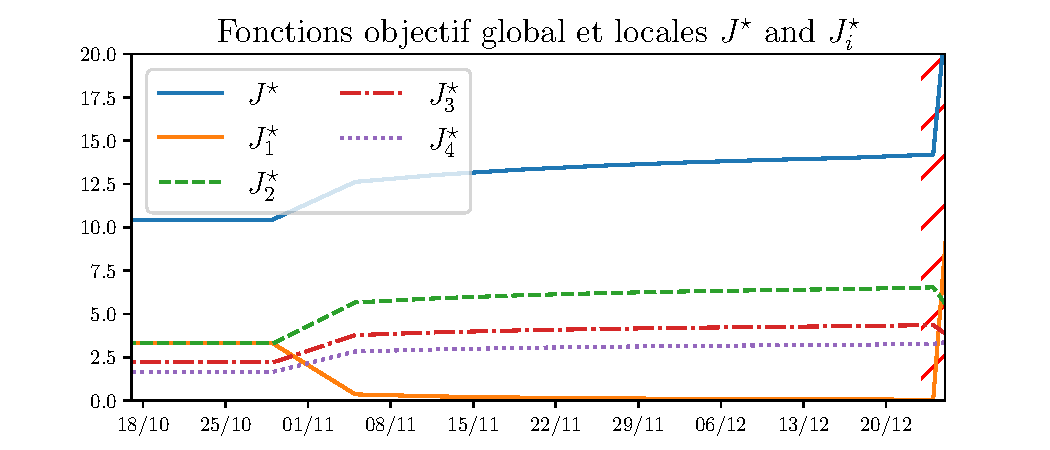
\includegraphics[width=.8\textwidth]{../img/example_introduction/example_J_fr.pdf}
  \caption{Graphique des fonctions objectifs dans une période de 10 semaines.}\label{fig:change_in_j_fr}
\end{figure}

Cet example simple nous donne les effets d'un attaque: perte de performance et cassure du fonctionnement du système.
Le même peut arriver causé par des fautes.
Motivé par exemples réels comme les black-out de 2010 au Brési~\cite{Conti2010}, l'attaque Stuxnet au Iran en 2011~\cite{Langner2011}, et les attaques à une central électrique en Ukraine in 2016~\cite{Bindra2017} et mal-heusement beaucoup d'autres~\cite{DingEtAl2018,DibajiEtAl2019}, on veut étudier la sécurité des \cps{}.

Dans ce travail on va focaliser sur la securité des \cps{} commandé par \dmpc{}.
On focalise dans le cas qu'ils sont attaqués par un agent mal intentionné, qui change le valeurs de quelques variables pour son propre bénéfice. Comme on verra cet attaque normalement est appelé an attaque de type \fdi{}.

Utilisant la connaisance acquise on propose des méthodes pour sécuriser ses systèmes.

On utilise comme guide les questions suivantes:
\simplebox{
  \begin{itemize} \bfseries
    \item Peut-on detecter l'attaque?
    \item Peut-on identifier l'attaquant?
    \item Peut-ont miniser les effets du dit attaque?
  \end{itemize}
}
Cette thèse a comme objectif répondre ces questions dans un cas spécifique qui sera formalement presenté.
Pour mieux comprendre et répondre ces questions, on divise ce travail en deux parties:

\paragraph{La première partie} (\S\ref{sec:comm-pred-et} à~\ref{sec:comp-anorm}) sert comme une gentille introduction au déssin des \dmpc{}, à sa sécurité et à des attaques.
\newcommand{\tpc}{\textperiodcentered}

Pour un\tpc{}e lecteur\tpc{}ice pas familiarisé\tpc{}e, Section~\ref{sec:comm-pred-et} explique ce qui est une Commande Prédictive et les défis pour la décomposer.
Section~\ref{sec:differents-topologies} discute les topologies possibles pour fair la décomposition.
Section~\ref{sec:comp-anorm} définit comportements anormaux, donne quelques exemples, les catégorise et présente les méthodes pour les prévenir et combattre.

\paragraph{La seconde partie} (\S\ref{sec:vulnerabilites-de-la} à~\ref{sec:comm-pred-resil-1}) contient les contributions de cette thèse.

Section~\ref{sec:vulnerabilites-de-la} présente la décomposition étudié (décomposition primale). On presents ses vulnérabilités et comment elles peuvent affecter la perfomance du système.
On formalise l'example en donnant une approche plus quantitative.
Une fois les vulnérabilités et les possibles effets des attaques découverts, on divise la mitigation en parties plus gérable.
\\ Premièrement en Section~\ref{sec:comm-pred-resil}, on analyse un problème simple, pour qu'on puisse apprécier les possibles difficultés qui peuvent être rencontrées pendant le problème de mitigation.
À partir de cette analyse, on propose des mécanismes de detection et mitigation, suivis par un example académique pour illustrer leur fonctionnement.
\\Après, en Section~\ref{sec:comm-pred-resil-1}, on analyse un problème similaire mais avec un coup de théâtre. Comme on verra, une petite modification du problème inital cause une augmentation exponentiel de sa complexité.
L'analyse de ce nouvel problème résulte une stratégie similaire, mais avec modifications adéquates pour renfermer la nature exponentiel du problème.

Finallement, on conclue le travail avec Section~\ref{sec:conclusion_fr}, où on discute les résultats de l'étude, ses bénéfices et inconvénients.
La discussion ouvre des questions qui peuvent inciter des nouveau travaux.
\subsection{Contributions}
Comme un contribution mineure, on démontre l'étude de la vulnérabilité des \dmpc{} basées sur la décomposition primale, qu'au meilleur de nos connaissance n'a pas jamais été étudié.

Comme contributions majeures, deux stratégies de mitigation pour types différents de système de complexité croissante.

La première pour des systèmes lesquels les ressources ne sont pas suffisants pour répondre aux nécessités des agents locaux, on les appelle \textbf{Systèmes Dépourvus}.

La seconde, pour une classe des systèmes exponentielment plus complexes, où on assume que les demandes locales respect au moins quelques contraintes. On utilise tel hypothèse pour acquérir des informations en utilisant une méthode qu'on appelle \textbf{pénurie artificielle}.

\subsection{Publications}
Les discussion dans cette thèse a donné comme résultats les publications suivantes:
\begin{itemize}
  \item Publiés
        \begin{description}
          \item[\cite{NogueiraEtAl2021}] Conference article for the SysTol'21
          \item[\cite{NogueiraEtAl2022}] Conference article for the NecSys'22
        \end{description}
\end{itemize}

\newpage
\section{Commande Prédictive et sa décomposition}\label{sec:comm-pred-et}

La commande prédictive basée en modèle, ou commande prédictive, ou encore \mpclong{} en anglais, est une stratégie de commande en boucle fermée basée dans la solution des problèmes d'optimisation.
Ayant un modèle du système à commander et une fonction objectif, la stratégie utilise le modèle pour prévoir l'évolution de ses états et computer une séquence optimale de command qui optimise la fonction donnée.
Comme on utilise des problèmes d'optimisation, il est naturel d'ajouter des restriction en forme de contraintes d'égalité et d'inégalité.

Cette stratégie a une place spéciale dans l'industrie et est présente dans une plethora d'applications (gestion d'énérgie~\cite{AnandutaEtAl2018}, commande des quadrotors~\cite{BanguraMahony2014} et autres).

Dans ce travail, on focalise sur la \mpc{} pour des systèmes linéaires avec entrées contraintes.

\subsection{\mpc{} pour des systèmes linéaires}\label{sec:mpc-pour-des}
Comme la \mpc{} est normalement développée en utilisant un ordinateur digital et la transmission des signaux continus peuvent demander une bande passante infinite~\cite{HeEtAl2022}, naturellement on utilise un modèle de temps discret pour le système a commander:
\begin{equation}\label{eq:large_scale_system_model_fr}
  \begin{array}{rclll}
    \vec{x}[k+1]&=&f(\vec{x}[k],\vec{u}[k])&=&A\vec{x}[k]+B\vec{u}[k]\\
    \vec{y}[k]&=&C\vec{x}[k]&&
  \end{array}
\end{equation}
où $\vec{x}[k]\in\R^{n_{x}}$ est l'état du système et $\vec{u}[k]\in\R^{n_{u}}$ est l'entrée.

On suppose que les entrèes du système sont contraintes par des contraintes affines comme
\begin{equation}
  \label{eq:linear_constraint_fr}
  \Gamma\vec{u}[k]\preceq\vec{u}_{\max},
\end{equation}
avec $\Gamma$ de taille adéquate $\R^{\card{\vec{u}_{\max}}\times n_{u} }=\R^{n_{c}\times n_{u} }$.

On suppose qu'on a un objectif de commande $\vec{v}$,
qui peut être \emph{rejeter perturbations}, où ${ \vec{v}[k]=\vec{x}[k] }$, ou \emph{suivi de trajectoire}, où ${ \vec{v}[k]=\vec{w}[k]-\vec{x}[k] }$, soit $\vec{w}[k]$ la trajectoire à suivre.
On utilise comme example le suivi de trajectoire de sortie (utilisant les relations entre $\vec{x}[k]$ et $\vec{y}[k]$), mais tout les résultats de ce travail sont aussi valable pour l'autre objectif.

La \mpc{} trouve une séquence d'entrées ${\vec{U}^{\star}[k]=[\vec{u}^{\star}[0|k];\dots; \vec{u}^{\star}[\predhorz-1|k]]}$ prédite dans un horizon $\predictionSet=\{1\mathbin{:}\predhorz\}$ qui minimiser la fonction ${J:\R^{n_{x}}\times\R^{\predhorz\cdot n_{u}}\to \R}$, définie comme
\begin{equation}
  \label{eq:quadratic_objective_with_sum_fr}
  J(\vec{x}[0|k],\vec{U}[k])=\sum_{i\in\predictionSet}\left[\norm{\mpcvec{v}[ ][i][k]}^{2}_{Q} +\norm{\mpcvec{u}[ ][i-1][k]}^{2}_{R}\right].
\end{equation}
Cette fonction, quand minimisée, doit assurer l'objectif $\vec{v}[k]$ choisi en minisant l'énérgie de l'entrée.
Les matrices ${ Q\in\semidefpos }$ et ${ R\in\defpos }$ sont des poids qui représentent les coûts respectives de chaque terme de l'équation.

En mettant en form matriciel, le problème résolu par la \mpc{} est le suivant
\begin{equation}
  \small
  \begin{aligned}
    \begin{matrix}
      \minimiser\limits_{\vec{U}[k]} &\norm{\vec{V}[k]}^{2}_{\bar{Q}} + \norm{\vec{U}[k] }^{2}_{\bar{R}}&\\
      \mathrm{sous} &
      \vec{x}[i|k]=A\vec{x}[i-1|k]+B\vec{u}[i-1|k]
      &
       \forall i\in\predictionSet \\
      &\bar{\Gamma}\vec{U}[k]\preceq {\vec{U}}_{\text{max}}&

    \end{matrix}
  \end{aligned}
  \label{eq:general_qp}
  \quad,
\end{equation}
où
\begin{align}
  \label{eq:construction_Gamma_fr}
  \bar{\Gamma}&=\kron{I_{\predhorz}}{\Gamma}\\
  \label{eq:construction_Umax_fr}
  \vec{U}_{\max}&=\kron{\1_{\predhorz}}{\vec{u_{max}}}\\
  \bar{Q}&=\kron{I_{\predhorz}}{Q}\\
  \bar{R}&=\kron{I_{\predhorz}}{R}.
\end{align}

En choisissant l'approche \emph{batch}~\cite[Chapter 8.2]{BorrelliEtAl2017}, on peut récrire le problème comme
\begin{equation}
  \label{eq:quadratic_objective_compact_batch_fr}
  \begin{aligned}
    \begin{matrix}
      \minimiser\limits_{\vec{U}[k]} &
      \norm{\vec{U}[k]}^{2}_{H} + 2{\vec{f}[k]}^{T}\vec{U}[k] + c[k] &\\
      \mathrm{sous} & \bar{\Gamma}\vec{U}[k]\preceq {\vec{U}}_{\text{max}}
    \end{matrix}
  \end{aligned}
\end{equation}
où, pour le suivi de trajectoire,
\begin{align}
  \label{eq:construction_H}
H&=\norm{\mathcal{Y}^{u}}^{2}_{\bar{Q}}+\bar{R}\\
\vec{f}[k]&={\mathcal{Y}^{u}}^{T}\bar{Q}(\mathcal{Y}^{x}\vec{x}[0|k]-\vec{W}[k])\\
c[k]&=\norm{\mathcal{Y}^{x}\vec{x}[0|k]}^{2}_{\bar{Q}}-2{\vec{W}[k]}^{T}\bar{Q}{\mathcal{Y}^{x}}\vec{x}[0|k]+\norm{\vec{W}[k]}^{2}_{\bar{Q}}.
\end{align}
avec les prédictions
\begin{equation}
    \begin{matrix}
      \underbrace{
        \left[
          \begin{matrix}
            \vec{y}[1|k] \\
            \vec{y}[2|k] \\
            \vdots \\
            \vec{y}[\predhorz|k]
          \end{matrix}
        \right]
      }_{\textstyle \vec{Y}[k]} &=&
      \underbrace{
        \left[
          \begin{matrix}
            CA^{1} \\
            CA^{2} \\
            \vdots \\
            CA^{\predhorz}
          \end{matrix}
        \right]
      }_{\textstyle \mathcal{Y}^{x}}
      \vec{x}[0|k]+
      \underbrace{
        \left[
          \begin{matrix}
            CA^{0}B & 0 & \dots & 0 \\
            CA^{1}B& \ddots & \ddots & \vdots      \\
            \vdots     & \ddots   & \ddots & \vdots    \\
            CA^{\predhorz-1}B & \dots & \dots & CA^{0}B
          \end{matrix}
        \right]
      }_{\textstyle \mathcal{Y}^{u}}
      \vec{U}[k]
    \end{matrix}
    \quad.
\end{equation}

Si on divise la fonction objectiv par $2$ et on ignore le terme constant $c[k]$, on a la structure standard d'une forme de programmation quadratique, connue comme \qp{}:
\begin{equation}
  \label{eq:qp_standard_form_fr}
  \begin{aligned}
    \begin{matrix}
      \minimiser\limits_{\vec{U}[k]} &
      \frac{1}{2}\norm{\vec{U}[k]}^{2}_{H} + {\vec{f}[k]}^{T}\vec{U}[k] &\\
      \mathrm{sous} &
\bar{\Gamma}\vec{U}[k]\preceq {\vec{U}}_{\text{max}}
    \end{matrix}
  \end{aligned}.
\end{equation}
\begin{remark}\label{rem:equivalence_problems_not_same_objective_fr}
  Observe que les problèmes~\eqref{eq:qp_standard_form_fr} et~\eqref{eq:quadratic_objective_compact_batch_fr} sont equivalents (même solution), mais ils ne sont pas le même problème, alors si on doit calculer la fonction objectif~\eqref{eq:quadratic_objective_compact_batch_fr} on doit utiliser la bonne version.
\end{remark}

La communauté de la \mpc\ utilise beaucoup les \qp{}, une fois qu'existe
une grande quantité de solveurs mathematiques pour les résoudre, on peut citer comme exemples le solveur interne de MATLAB\footnote{\url{https://fr.mathworks.com/help/optim/ug/quadprog.html}}, OSQP\footnote{\url{https://osqp.org}}, MOSEK\footnote{\url{https://www.mosek.com}} et aussi ECOS\footnote{\url{https://github.com/embotech/ecos}}.

Par contre, la solution dans cette forme \textbf{monolithique} peut être intensive au niveau de calcul, dépendant des valeurs de $n_{x}$, $n_{u}$, $n_{c}$ and $\predhorz$.
Pour améliorer la solution on utilise des méthodes de décomposition.
On peut décomposer en différents échelles de temps~\cite{ChenEtAl2011}, utilisant théorie des jeux~\cite{MaestreEtAl2011} ou algorithmes génétiques associés avec des observateur d'états~\cite{XieEtAl2016}.
Mais dans ce travail on utilise des techniques de décomposition basées dans la décompostion de problèmes d'optimisation~\cite{GiselssonEtAl2013}.

\subsection{Décomposition de problèmes d'optimisation}\label{sec:decomp-de-probl}
Comme montré en~\cite{ConejoEtAl2006} et~\cite{BoydEtAl2015}, un problème d'optimisation est décomposable s'il y a plus qu'une variable de decision et on peut le diviser en au moins deux sub-problèmes.

Si les sous-problèmes ne sont pas couplés, on peut les résoudre en parallel et la solution est trouvée, sans aucune interaction entre les sous-problèmes.
Cependant, s'ils sont couplés, on doit utiliser une méthodologie pour trouver la bonne solution.

Les problèmes peuvent être couplés par variables ou par contraintes, ces variables et contraintes sont appelées compliquants.
Comme vue en~\cite{BoydEtAl2015}, une contrainte compliquant le problème peut être transformée en une variable qui complique le problème et vice versa.
Dans ce travail on utilise juste les contraintes compliquantes.

L'idée générale est de prendre un problème décomposable comme
\begin{equation}\label{eq:general_coupled_optimization_problem_fr}
  \small
  \begin{aligned}
    \begin{matrix}
      \minimiser\limits_{\text{variables de decision}}  &\text{objective}_{1}&+&\text{objective}_{2}&\\
      \mathrm{sous} & \text{constraintes}_{1},&&  \text{constraintes}_{2}\\
      &&\text{contraintes compliquantes}_{12}&
    \end{matrix}
  \end{aligned}
\end{equation}
et le récrire comme un problème équivalent avec des variables auxiliaires, comme
\begin{equation}\label{eq:general_coupled_optimization_problem_decomposed_main_problem_fr}
  \small
  \begin{aligned}
    \begin{matrix}
      \minimiser\limits_{\mathop{\operatorname{+}}\limits^{\text{variables de decision}}_{\text{variables auxiliaires}}}  &\text{objective}^{*}_{1}(\text{variables auxiliaires })+\text{objective}^{*}_{2}(\text{variables auxiliaires})&\\
    \end{matrix}
  \end{aligned}
\end{equation}
où $\text{objective}^{*}_{1}(\text{variables auxiliaires})$ et $\text{objective}^{*}_{2}(\text{variables auxiliaires})$ sont calculés en résolvant les sous-problèmes
\begin{subequations}\label{eq:general_coupled_optimization_problem_decomposed}
\begin{equation}\label{eq:general_coupled_optimization_problem_decomposed_1}
    \begin{matrix}
      \minimiser\limits_{\text{variables de decision}_{1}}  &\text{objective}_{1}&\\

      \mathrm{sous} & \text{constraints}_{1}\\
      &\text{contraintes compliquants}_{12_{1}}(\text{variables auxiliaires}_{1})
    \end{matrix}
\end{equation}
\begin{equation}\label{eq:general_coupled_optimization_problem_decomposed_2}
    \begin{matrix}
      \minimiser\limits_{\text{variables de decision}_{2}}  &\text{objective}_{2}&\\

      \mathrm{sous} & \text{constraints}_{2}\\
      &\text{contraintes compliquants}_{12_{2}}(\text{variables auxiliaires}_{2})
    \end{matrix}
\end{equation}
\end{subequations}
dont les solutions dépendent de ces variables auxiliaires ajoutées.
Pour trouver la valeure optimale des variables auxiliaires, il est nécessaire la coordination des sous-problèmes.


Le problème equivalent est appelé \emph{problème principal}, il est résolu par la coordination entre les sous-problèmes en utilisant la mise à jour des variables auxiliaires, appelées \emph{variables d'interface}.
Les méthodes de mis à jour sont basées sur un algorithme d'optimisation, comme
la bisection, plans sécants, ou d'autres méthodes qui utilisent le (sub)gradient ou des approximations.
La dernière classe est la plus utilisée, et quelques exemples sont l'iteration de Arrow-Hurwicz-Uzawa~\cite{BourdaisEtAl2012}, sub-gradient projeté~\cite{BiegelEtAl2012}, et la plus forte descente~\cite{BoydEtAl2011}.
La forme exacte depend de la topologie utilisée (discuté en \S\ref{sec:differents-topologies}).

Les sous-problemès, on les appelle \emph{problèmes locaux}.
Ils sont obtenus en utilisant des méthodes d'equivalence entre problèmes d'optimisation~\cite{BoydVandenberghe2004}, comme le problème original (primal)~\cite{PaulenEtAl2016, CamisaEtAl2022}, le dual ~\cite{MorosanEtAl2011, BourdaisEtAl2012,VelardeEtAl2018}, utilisant des opérateur comme l'opérateur proximal~\cite{Iiduka2019,OconnorVandenberghe2014}, ou d'autres stratégies.

Les \emph{problèmes locaux} ont un ensemble de contraintes formé par les contraintes derivées des contraintes décomposables du problème original, appelées \emph{contraintes locales}, et quelques autres contraintes derivées de la partie compliquante, \emph{contraintes globales d'accouplement}.
La solution de cette partie des contraintes d'accouplement dépendent des variables d'interface.

Les variables d'interface dépendent des problèmes locaux choisis.
Par example, pour des problèmes primaux, normalement les variables duales sont utilisées~\cite{Cohen1978}; pour les problèmes duals, le résidu des contraintes~\cite{BoydEtAl2015}; et pour la méthode d'alternance de direction des multiplicateurs, en anglais \ADMM, variables primales et autres multiplicateurs sont utilisés (la mise à jour de ses multiplicateurs donnent le nom de la méthode)~\cite{BoydEtAl2011}.

Ce travail se concentre à la décomposition primale et utilise le sub-gradient projeté.
Cette décomposition sera expliquée dans une section future (\S\ref{sec:vulnerabilites-de-la}).
Pour d'autres exemples on réfère~\cite{MaestreEtAl2014} ou~\cite{ConejoEtAl2006}.

\newpage
\section{Differents topologies}\label{sec:differents-topologies}
Comme dit, la forme de la décomposition dépend dans la topologie utilisé pour résoudre le problème.
Dans cette section on montre le différentes classification des topologies.

\subsection{Par distribution des unités de computation}\label{sec:par-distribution-des}

La première forme de catégoriser la topologie est par comme on distribue les unités de computation.

Ces unités peuvent être géographiquement séparés ou pas (même hardware) dépendant de l'échelle du \cps{} controllé.
Si le système a une grande échelle et peut être distribué géographiquement, naturellement on essaye de positionner le hardware stratégiquement pour correspondre aux sous-systèmes, mais pas toujours il est possible.
On peut voir dans la Fig.~\ref{fig:corresponding_noncorresponding_fr} des exemples quand les sous-problèmes correspondent ou pas aux sous-systèmes.
\begin{figure}[h] \centering
  \begin{subfigure}{.4\textwidth}
    \centering
    \def\svgwidth{.8\textwidth}
    \input{../img/noncorresponding_topology.pdf_tex}
    % 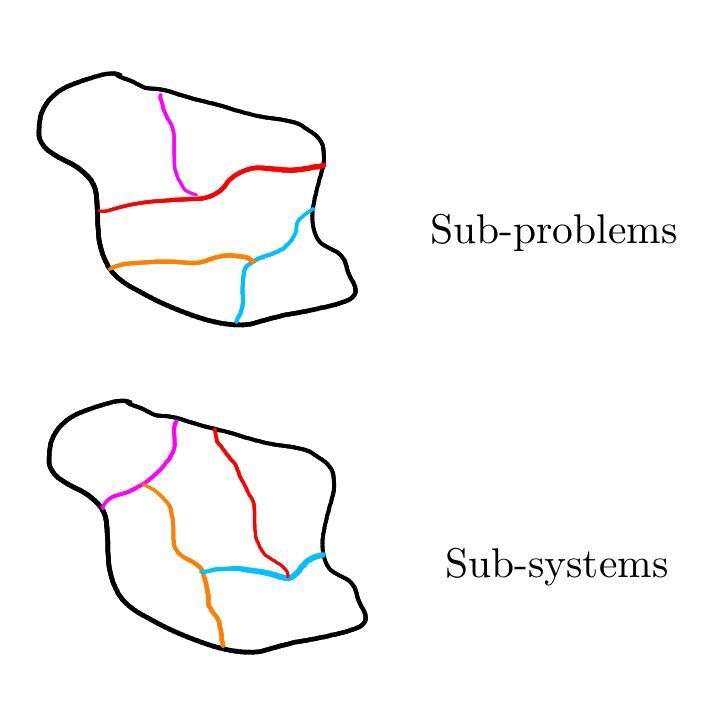
\includegraphics[width=\textwidth,clip,trim=0cm 1.8cm 0 2.5cm]{../img/noncorresponding_system_problem.png}
    \caption{Non correspondant.}\label{fig:noncorresponding_division_system_problem}
  \end{subfigure} \hfill
  \begin{subfigure}{.4\textwidth} \centering
    \def\svgwidth{.8\textwidth}
    \input{../img/corresponding_topology.pdf_tex}
    % 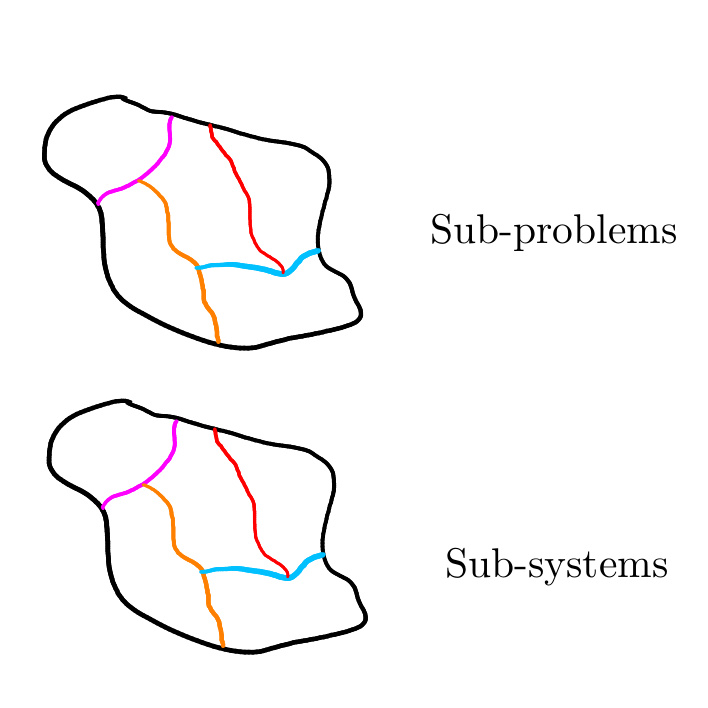
\includegraphics[width=\textwidth,clip,trim=0cm 1.8cm 0 2.5cm]{../img/corresponding_system_problem.png}
    \caption{Correspondant.}\label{fig:corresponding_division_system_problem}
  \end{subfigure}
  \caption{Décomposition du problèmes en ($P_i$) et du système en ($S_{i}$).}\label{fig:corresponding_noncorresponding_fr}
\end{figure}

Dans la littérature, c'est normal de choisir les unités de façon que ça correspond comme en Fig.~\ref{fig:corresponding_division_system_problem}~\cite{ArauzEtAl2021}, alors, dans ce travail on considère aussi que les sous-problèmes et sous-systèmes \textbf{correspondent}.
De cette façon, les termes sous-problèmes, sous-systèmes, agents et unités seront utilisés indistinctement.

\subsection{Par communication}\label{sec:par-communication}

Normalement, comme montré en \S\ref{sec:decomp-de-probl}, la communication n'est pas nécessaire si les sous-problèmes ne sont pas couplés.
Cependant, il existe des cas pour la \dmpc{} où on peut exploiter des propriétés de robustess de la \mpc{} pour computer la solution sans communication~\cite{VahidNaghaviEtAl2014}.
Pour d'autres decomposition d'optimisation il est possible montrer que dans certaines circonstances la communication n'est pas nécessaire non plus~\cite{VoulgarisElia2022}.
\begin{remark}
  Généralement, dans la littérature de la \dmpc{} le terme ``décentralisé'' se refère aux méthodes où les agents ne se communiquent~\cite[\S 4]{ChristofidesEtAl2013},\cite{NegenbornMaestre2014}.
  Mais le terme peut être confus et dans certains cas même ``mal-utilisé''.
  Donc, on opte pour une nomenclature différente, an appellant ces méthodes comme ``contrôle non coordonné'', une fois qu'il n'y a pas de coordination entre agents ni un agent coordinateur.
  On utilise le terme ``décentralisé'' comme opposé de ``centralisé'' (monolithique), i.e.\ pour décrire structure au lieu de la communication.
\end{remark}

Comme dans la majorité de la littérature où grande part des contrôles son coordonnés~\cite{NegenbornMaestre2014, ArauzEtAl2021}, dans \textbf{ce travail}, on suppose aussi que les agents se communiquent.
On considère aussi qu'il existe au moins un chemin de communication entre tous les agents (le \textbf{graphe} équivalent est \textbf{connecté}).

\subsection{Par relations de pouvoir}\label{sec:par-relations-de}
Une autre classification est par l'influence que les agents exercent les uns sur les autres.
Par example, quelques agents peuvent avoir plus de pouvoir (être plus importants) qu'autres.
Ce genre de relation est appellé hiérarchique, normalement le pouvoir est démontré par le différentes types d'actions réalisées par les agents.
Normalement les plus importants ont des rôles de médiateur, certificateur, régulateur et etc.
Pour les systèmes où il n'y a pas de différence de comportement ou d'influence entre les agents, on les appelle anarchiques.
Dans Fig.~\ref{fig:hierarchic_anarchic_fr} on voit des exemples de ces deux types de structures.
\begin{figure}[h]
\begin{subfigure}[b]{.45\textwidth}
  \centering
  \scalebox{1.5}{
  \begin{tikzpicture}[node distance=.5cm and .5cm,inner sep=0pt,every node/.style={minimum width=0.1cm}]
    \node[draw,circle,minimum width=.7cm] at (0,0) (first) {};
    \node[draw,circle,below left=of first,minimum width=.4cm] (second_l) {};
    \node[draw,circle,below right=of first,minimum width=.4cm] (second_r) {};

    \node[draw,circle,below left =0.8cm and 0.1cm  of second_l,minimum width=.2cm] (third_1) {};
    \node[draw,circle,below right=0.8cm and -0.0cm of second_l,minimum width=.2cm] (third_2) {};
    \node[draw,circle,right      =1.8cm and 0.5cm    of third_2   ,minimum width=.2cm] (third_3) {};
    \node[draw,circle,below left =0.8cm and -0.0cm of second_r,minimum width=.2cm] (third_4) {};
    \node[draw,circle,below right=0.8cm and 0.1cm  of second_r,minimum width=.2cm] (third_5) {};

    \draw[-]  (first)  -- (second_l);
    \draw[-]  (first)  -- (second_r);
    \draw[-]  (second_l) -- (third_1);
    \draw[-]  (second_l) -- (third_2);
    \draw[-]  (second_l) -- (third_3);
    \draw[-]  (second_l) -- (third_5);
    \draw[-]  (second_r) -- (third_2);
    \draw[-]  (second_r) -- (third_3);
    \draw[-]  (second_r) -- (third_4);
    \draw[-]  (second_r) -- (third_5);
  \end{tikzpicture}
  }
  \caption{Hierarchie.}\label{fig:hierarchy_topology_fr}
\end{subfigure}
\hfill
\begin{subfigure}[b]{.45\textwidth}
  \centering
  \scalebox{1.5}{
  \begin{tikzpicture}[node distance=.5cm and .5cm,inner sep=0pt,every node/.style={minimum width=0.3cm}]
    \node[draw,circle] at (0,0) (a) {};
    \node[draw,circle] at ($(a)+(-.7,-.3)$) (b) {};
    \node[draw,circle] at ($(a)+(0.0,-0.8)$) (c) {};
    \node[draw,circle] at ($(a)+(0.8,-0.4)$) (d) {};
    \node[draw,circle] at ($(b)+(0.1,-1.0)$) (e) {};
    \node[draw,circle] at ($(e)+(1.2,-0.1)$) (f) {};
    \node[draw,circle] at ($(f)+(0.6,0.4)$) (g) {};
    \node[draw,circle] at ($(e)+(-0.8,-0.0)$) (h) {};
    \node[draw,circle] at ($(f)+(-0.5,-0.5)$) (i) {};

    \draw[-]  (a)  -- (b);
    \draw[-]  (a)  -- (c);
    \draw[-]  (a)  -- (d);
    \draw[-]  (b)  -- (c);
    \draw[-]  (c)  -- (d);
    \draw[-]  (e)  -- (b);
    \draw[-]  (e)  -- (c);
    \draw[-]  (c)  -- (f);
    \draw[-]  (d)  -- (g);
    \draw[-]  (f)  -- (g);
    \draw[-]  (e)  -- (h);
    \draw[-]  (f)  -- (i);
  \end{tikzpicture}
  }
  \caption{Anarchie}\label{fig:anarchy_topology_fr}
\end{subfigure}
\caption[Topologies hierarchiques et anarchiques.]{Topologies hierarchiques et anarchiques. \\Noeuds plus grands représentent plus de pouvoir/influence sur autres.}\label{fig:hierarchic_anarchic_fr}
\end{figure}

Quelques fois la structure est impliquée par la décomposition.
Par example, il y a des décomposition où des agents résolvent leur problèmes un après l'autre jusqu'à qu'il aye une convergence
(Fig.~\ref{fig:sequential_topology_fr})~\cite{LiuEtAl2009a}.
Ces schémas sont appelés \emph{séquentiels}.
L'hierarchie est impliqué une fois que le premier agent résout son problème en ignorant les autres, lui donnant, même que juste temporairement, une position de pouvoir.

En quelques autres les agents résolvent ses problèmes indépendamment et partagent quelques résultats jusqu'à un consensus soit trouvé, itérativement ou pas (Fig.~\ref{fig:parallel_topology_fr})~\cite{LiuEtAl2010}.
Ces structure sont appelées \emph{parallèles} et il n'a pas d'hierarchie.
\begin{figure}[h]
\begin{subfigure}[b]{.45\textwidth}
  \centering
  \begin{tikzpicture}[node distance=1cm and .5cm]
    \node[draw,circle] (first) at (0,0) {};
    \node[draw,circle,right=of first] (second) {};
    \node[draw,circle,right=of second] (third) {};
    \node[draw,circle,opacity=0,right=of third] (fourth) {};
    \node[draw,circle,right=of fourth] (fifth) {};

    \node[] at (fourth) {...};
    \draw[-latex] (first) -- (second);
    \draw[-latex] (second) -- (third);
    \draw[-latex] (third) -- (fourth);
    \draw[-latex] (fourth) -- (fifth);
  \end{tikzpicture}
  \caption{Topologie séquentiel.}\label{fig:sequential_topology_fr}
\end{subfigure}
\hfill
\begin{subfigure}[b]{.45\textwidth}
  \centering
  % 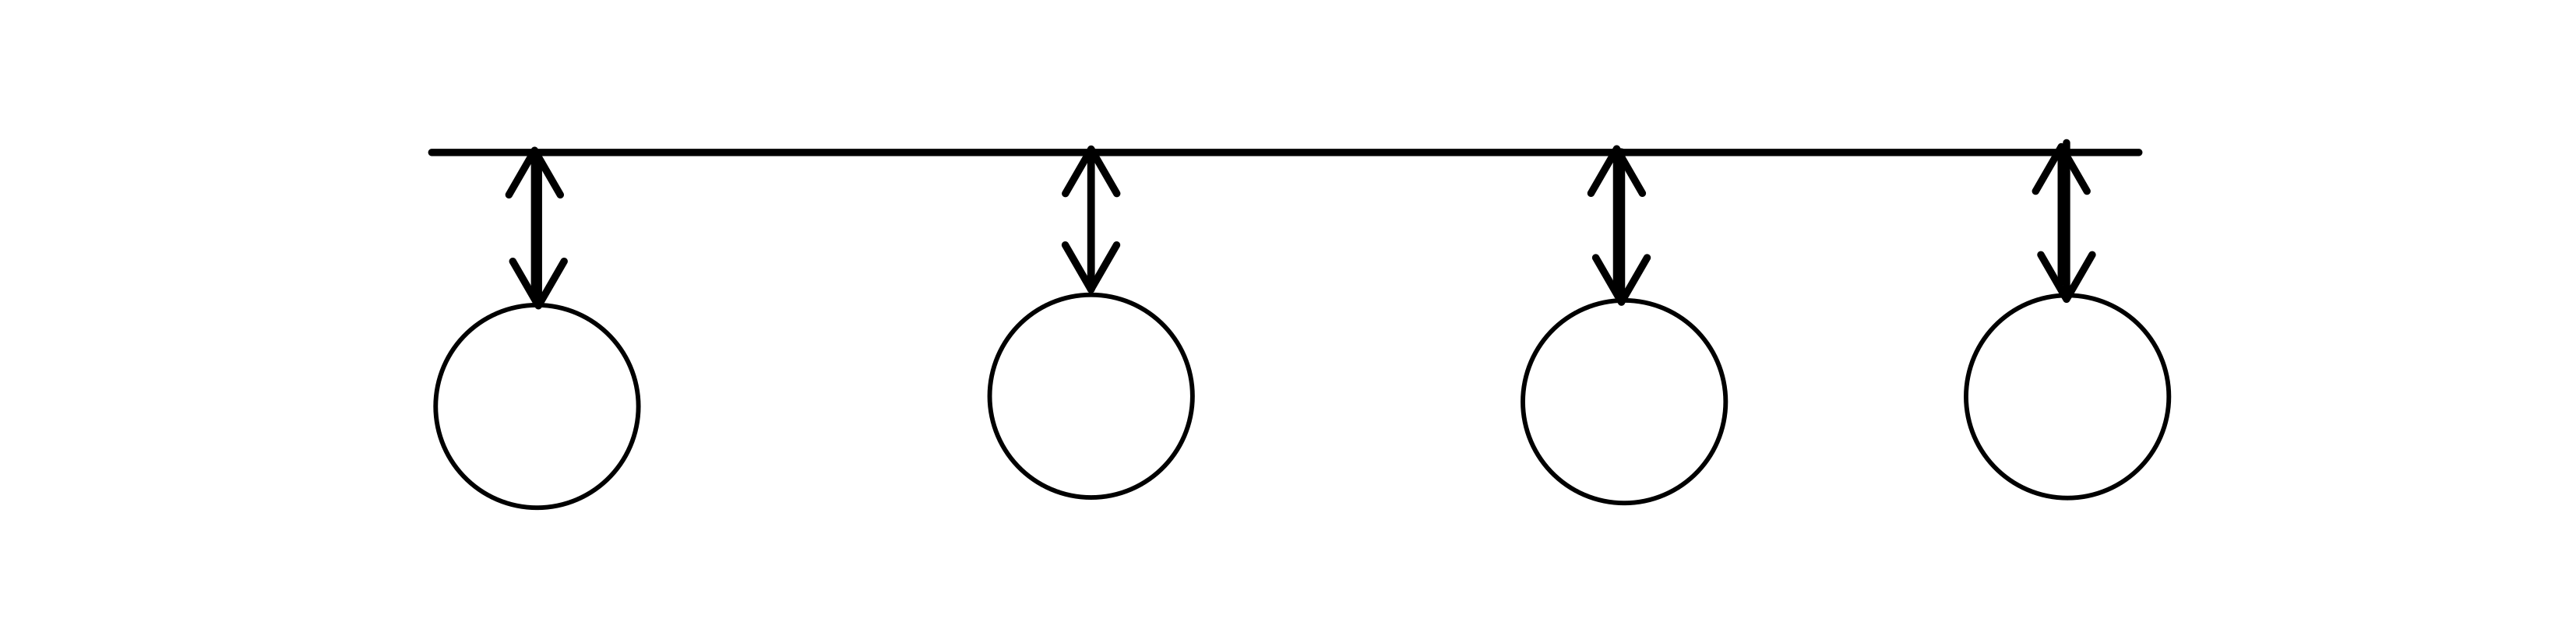
\includegraphics[width=\textwidth]{../img/parallel_topology.png}
  \begin{tikzpicture}[node distance=.5cm and .5cm,inner sep=0pt,minimum width=.5cm]
    \node[draw,rectangle,fill=black,minimum height=2pt,minimum width=5cm] (bar) at (0,0) {};
    % \draw[blue,fill] ($(bar)+(-2.5cm,-2pt)$) rectangle ($(bar)+(2.5cm,2pt)$);
    \node[draw,circle,below=of bar] (third) {};
    \node[draw,circle,left=of third] (second) {};
    \node[draw,circle,left=of second] (first) {};
    \node[draw,circle,opacity=0,right=of third] (fourth) {};
    \node[draw,circle,right=of fourth] (fifth) {};

    \node[] at (fourth) {...};
    \draw[latex-latex]  (first)  -- (bar.south -| first);
    \draw[latex-latex]  (second) -- (bar.south -| second);
    \draw[latex-latex]  (third)  -- (bar.south -| third);
    \draw[latex-latex]  (fifth)  -- (bar.south -| fifth);
  \end{tikzpicture}
  \caption{Topologie parallèle.}\label{fig:parallel_topology_fr}
\end{subfigure}
\caption{Topologies séquentiel et parallèle.}\label{fig:sequential_parallel_topology_fr}
\end{figure}

Dans d'autres cas, on peut choisir par l'hiérarchie ou anarchie.
Ça dépendant normalement de comment se passent les relations de confiance entre les possibles agents.
On peut choisir faire confiance à quelques agents pour l'échange des informations, ainsi comme on fait dans la vrai vie avec le système financier, agences d'inspection et régulation dans différent domaines.
En~\cite{McNamaraEtAl2018} et~\cite{OlaruEtAl2018}, on voit le parallèle entre les structures de commande et les relations politiques/sociétales.

Dans ce travail on utilise une structure hierarchique qui sera mieux décrite en
\S\ref{sec:vulnerabilites-de-la}.

\subsection{Par type de communication}\label{sec:par-type-de}

Le type de communication peut aussi être utilisé pour catégoriser les topologies,
Les agents peuvent se communiquer uni ou bi-directionnellement.
Si les agents utilisent un schéma de communication bi-directionel, il est plus simple à gérer, une fois qu'ils peuvent se communiquer directement.
Par contre si le schéma est uni-directionel il faut utiliser des autres moyens pour prouver leur comunication (s'il existe un chemin entre eux), ou pour prouver la convergence des algorithmes~\cite{GarinSchenato2010}.

Une autre classification par type de communication c'est si la communication est synchrone ou asynchrone.
En générale, les schémas synchrone sont plus simples, alors que les asynchrone dépendent de politique de communication spécifiques.
Broadcast et gossiping~\cite{GarinSchenato2010} sont des exemples de ce type de communication.
\\Pour le broadcast (uni-directionnel), un agent transmet l'information à tout ses voisins sortant ($\set{N}_{\text{sortie}}$) et chaque destinataire met à jour ses variables locales.
\\Gossiping peut être divisé en deux, asymétrique et symétrique.
La version asymétrique (uni-directionel), l'agent choisit un des ses voisins sortant, et lui envoie l'information, le destinataire met à jour ses variables locales quand le message arrive.
De l'autre côté, dans le cas symétrique (bi-directionel), après avoir mis à jour les variables, le destinataire devient transmetteur, envoyant ses informations au expéditeur original, qui aussi met à jour ses propres variables une fois que ce nouvel message arrive.

Dans ce travail on suppose que les agents se communiquent bi-directionnellement et de manière synchrone.

\newpage
\section{Comportements anormaux}\label{sec:comp-anorm}
Comportements anormaux sont n'import quel comportement ou changement de comportement inattendu d'un système.

Les deux causes principales sont \emph{défauts} et \emph{attaques}.
La différence principale entre les deux est \emph{l'intention}.
Alors que défauts se passent involontairement, non coordonés et sans objectif, attaques sont intentionnel, généralement coordonés avec un objectif malicieuse.

Comme les deux peuvent changer le comportement du système nous sommes intéressés en maintenir l'opération normale des \cps{}.


\subsection{Security}\label{sec:security_fr}
La sécurité évoque l'opération sûre d'un système.
Pour ça, on utilise comme base la définition pour la cyber-sécurité et on l'étend pour les \cps{}.

La \emph{cyber-security} a trois pilliers: confidentialité, intégrité, et disponibilité, en anglais \CIA{}~\cite{Bishop2005}.

\paragraph{Confidentialité} des données et ressources.
Parfois on a besoin de mettre en secret quelques parties du système et on veut qu'il soit acessible pour un groupe privilégié.
Ça peut être pour raisons de privacité, pour eviter la diffusion des données personnels ou pour éviter l'exposition des vulnérabilités du système (un exemple dans la culture pop sont les plans de l'étoile noire de la saga Star Wars).

\paragraph{Intégrité} des données et ressources.
Un équipement nouveau est plus digne de confiance qu'un ancient qui a probablement souffert plus des intempéries.
Dans la transmission de données l'intégrité peut être divisé dans l'intégrité de l'information (l'information reçue est la même qu'a été envoyée) et l'intégrité de l'identité du expéditeur/destinataire (authentification).

\paragraph{Disponibilité} des données et ressources quand demandés par un utilisateur.
Comme mentionné en~\cite{Bishop2005}, ``un système indisponible est au moins aussi mauvais qu'aucun système du tout''.
\\~\\
Les vulnérabilités d'un système peut compromettre n'importe lequel de ces pilliers, parfois multiples au même temps.
\subsection{Vulnérabilités des \cps{}}

Les \cps{} ont des composant des domaines physiques et cyber.
On peut les diviser en partie matériel et immatériel.
Chacune de ces parties sont des points de vulnerabilité d'un \cps{}.

Dispositifs physiques comme des transducteurs (capteur/actionneur) peuvent être cibles de sabotage. Par example un attaquant peut utiliser un objet frais pour changer la lecture des capteurs de témperature d'une salle. Mais ils peuvent aussi se détériorer avec le temps ou d'autres accidents naturelles (chute d'arbres ,glissement de terres, attaques d'animaux, ouragans etc) et causer des défauts.

Le software peut aussi être une source de vulnérabilité à cause des \emph{bogues}, qui peut interrompre le fonctionnement du système ou même permettre un \emph{hacker} de s'infiltrer et gagner accès au système.
L'ordinateur utilisé pour la commande peut être mal dimensionné (puissance de calcul insuffisante), et recevoir plus de requêtes qu'attendu, arrivant à un état de surcharge cessant de répondre.


\subsection{Attaques in \cps{}}\label{sec:attacks_fr}

Il existe plusiers modèles de catégorisation de attaques en \cps{}.
Ici on montre les deux plus connus.
Le premier modèle est basé dans la cyber-security appélé 3D ou \DDDshort par l'acronyme anglais \DDD.
\textbf{Disclosure} est tout accès non autorisé à l'information (rupture de confidentialité).
\textbf{Deception} est l'idée d'utiliser de l'information fausse pour tromper quelqu'un (rupture d'intégrité).
\textbf{Disruption} est l'interruption du fonctionnement du système (rupture de la disponibilité). Aussi on peut ajouter l'\textbf{usurpation} d'identité (rupture de la authenticité).

On définit comme un attaque n'importe laquelle action mal-intentionné qui utilise les vulnérabilités d'un \cps{} à fin de violer sa sécurité.
L'agent est appellé attaquant.

Utilisant comme base~\cite{Bishop2005},~\cite{CardenasEtAl2008},~\cite{AminEtAl2009}, et autres, on peu créer une abstraction des \cps{} dans un réseau (Fig.~\ref{fig:networked_cps_abstraction_fr}).

\begin{figure}[h]
  \centering
\begin{tikzpicture}[node distance=1cm and 2cm,
    box/.style={draw,align=center,minimum height=1.5cm,minimum width=3cm,rectangle,black},
		]

    \node[box] (plant) at (0,0) {Système\\Physique};

    \node[box,below=of plant] (controller)  {Contrôleur};

    \node[draw,cloud,aspect=2,cloud puffs=20,below=1.5cm of controller] (network)  {Réseau};

    \draw[thick] (controller.west) -- ++(-1,0) node (a) {} node [midway,below] {${u}$};
    \draw[thick] (a.center) -- (a.center |- plant.west) node (b) {};
    \draw[-latex,thick] (b.center) -- (plant.west);

    \draw[thick] (plant.east) -- ++(1,0) node (aa) {} node [midway,above] {${y}$};
    \draw[thick] (aa.center) -- (aa.center |- controller.east) node (bb) {} ;
    \draw[-latex,thick] (bb.center) -- (controller.east);

    \draw[latex-,thick,dotted] (controller.south -| network.puff 20) -- +(0,-.25) node (nin) {} ;
    \draw[thick,dotted] (nin.center) -- ($(nin.center) + (0,-1)$) node (nin2) {};
    \draw[thick,dotted] (nin2.center) -- (network.puff 20) {};
    \node at ($(nin2)+(.45,.40)$) {$\mathcal{I}_{\text{ent}}$};

    \draw[latex-,thick,dotted] (network.puff 2) -- +(0,.25) node (nout) {} ;
    \draw[thick,dotted] (nout.center) -- ($(nout.center) + (0,1)$) node (nout2) {};
    \draw[thick,dotted] (nout2.center) -- ( controller.south -| network.puff 2) {};
    \node at ($(nout)+(-.45,.5)$) {$\mathcal{I}_{\text{sort}}$};
  \end{tikzpicture}
  \caption{Abstraction Générale d'un \cps{} dans un réseau.}\label{fig:networked_cps_abstraction_fr}
\end{figure}

Dans le diagramme, $u$ correspond à la commande calculé par le contrôleur et appliquée au système physique à travers des actionneurs. $y$ correspond aux sorties des capteurs du système.
Les signaux $I_{\text{ent}}$ et $I_{\text{sort}}$ sont les informations reçu et envoyées utilisant le réseau (envoyées ou venues d'autres sous-systèmes).

Avec le modèle \DDD{}, on peut catégoriser les attaques par où dans le système ils surviennent.
Dans la Fig.~\ref{fig:attacks_networked_cps_fr} on voit différents types d'attaques énumérés de A1 à A13.
Les attaques de A1 à A4 sont des attaques du type \emph{disclosure}, qui se passent au niveau de l'information.
L'attaquant observe le trafic d'information pour une utilisation postérieure.
Ce genre d'attaque est aussi appellé \textbf{snooping} ou \textbf{eavesdropping} (furetage et écoute illicite).
A5 à A8 representent attaques du type \emph{deception}.
Aussi au niveau informationnel, mais dans ce cas le signaux sont modifiés (representés par un \~{} dans le symbole de la variable).
Les attaques A10 à A12 sont du type \emph{disruption}, quand l'attaquant attaque le canal de c communication, empêchant la communication entre deux entités.
Et finallement, A13 sont des attaques physiques, ou le système physique est attaqué directement.
Cet attaque change physiquement le comportement du système.

\begin{figure}[h]
  \centering
  \begin{tikzpicture}[node distance=1cm and 2cm,
    box/.style={draw,align=center,minimum height=1.5cm,minimum width=3cm,rectangle,black},
		]

    \node[thick,box] (plant) at (0,0) {Système\\Physique};

    \node[thick,box,below=of plant] (controller)  {Contrôleur};

    \node[thick,draw,cloud,aspect=2,cloud puffs=20,below=2.0cm of controller] (network)  {Réseau};

    \draw[thick] (controller.west) -- ++(-1,0) node (a) {} node [midway,below] (input) {$\tilde{u}$};
    \draw[thick] (a.center) -- (a.center |- plant.west) node (b) {};
    \draw[-latex,thick] (b.center) -- (plant.west);
    \node (switch_input) at ($(a)!0.5!(b)$) {};

    \draw[thick] (plant.east) -- ++(1,0) node (aa) {} node [midway,above] (output) {$\tilde{y}$};
    \draw[thick] (aa.center) -- (aa.center |- controller.east) node (bb) {} ;
    \draw[-latex,thick] (bb.center) -- (controller.east);
    \node (switch_output) at ($(aa)!0.5!(bb)$) {};


    \draw[latex-,thick,dotted] (controller.south -| network.puff 20) -- +(0,-.5) node (nin) {} ;
    \draw[thick,dotted] (nin.center) -- ($(nin.center) + (0,-1)$) node (nin2) {};
    \draw[thick,dotted] (nin2.center) -- (network.puff 20) {};
    \node (info_in) at ($(nin)+(.45,-.10)$) {$\widetilde{\mathcal{I}_{\text{ent}}}$};

    \draw[latex-,thick,dotted] (network.puff 2) -- +(0,.5) node (nout) {} ;
    \draw[thick,dotted] (nout.center) -- ($(nout.center) + (0,1)$) node (nout2) {};
    \draw[thick,dotted] (nout2.center) -- ( controller.south -| network.puff 2) {};
    \node (info_out) at ($(nout)+(-.45,-.3)$) {$\widetilde{\mathcal{I}_{\text{sort}}}$};

    \node[red,above right=1cm of aa,inner sep=1pt,align=center] (a1) {\scalebox{1.5}{\faUserSecret}};
    \draw[-latex,thick] (a1) -- (output) node [midway,above,sloped] {{\faEye} A1} node [midway,below,sloped] {{\faPencil} A5};
    % \draw[-latex,thick] ($(a1)+(0,.1)$) -- ($(output)+(0,.1)$)  node [midway,above,sloped] {A1\faEye};
    % \draw[-latex,thick] ($(a1)+(0,-.1)$) -- ($(output)+(0,-.1)$)  node [midway,below,sloped] {A1\faPencil};


    \node[red,right=1.2cm of info_in,inner sep=1pt,align=center] (a2) {\scalebox{1.5}{\faUserSecret}};
    \draw[-latex,thick] (a2) -- (info_in) node [midway,below,sloped] {{\faEye} A2} node [midway,above,sloped] {{\faPencil} A6};

    \node[red,left=1.3cm of info_out,inner sep=1pt,align=center] (a3) {\scalebox{1.5}{\faUserSecret}};
    \draw[-latex,thick] (a3) -- (info_out) node [midway,above,sloped] {A3 {\faEye}} node [midway,below,sloped] {A7 \reflectbox{\faPencil}};


    \node[red,below left=1cm of a,inner sep=1pt,align=center] (a4) {\scalebox{1.5}{\faUserSecret}};
    \draw[-latex,thick] (a4) -- (input) node [midway,above,sloped] {A4 {\faEye}} node [midway,below,sloped] {A8 \reflectbox{\faPencil}};


    \node[red,right=.4cm of switch_output,inner sep=1pt,align=center] (a5) {\scalebox{1.5}{\faUserSecret}};
    \node[inner sep=1pt,align=center] at ($(switch_output) + (.3,0)$) {\rotatebox[origin=c]{180}{\faCut}};
    \node [above,sloped] at ($(a5) + (-.05,-.8)$) {A9};

    \node[red,right=.4cm of nin2,inner sep=1pt,align=center] (a6) {\scalebox{1.5}{\faUserSecret}};
    \node[inner sep=1pt,align=center] at ($(nin2) + (.3,0)$) {\rotatebox[origin=c]{180}{\faCut}};
    \node [above,sloped] at ($(a6) + (-.05,-.8)$) {A10};


    \node[red,left=.4cm of nout2,inner sep=1pt,align=center] (a7) {\scalebox{1.5}{\faUserSecret}};
    \node[inner sep=1pt,align=center] at ($(nout2) + (-.3,0)$) {\rotatebox[origin=c]{0}{\faCut}};
    \node [above,sloped] at ($(a7) + (-.05,-.8)$) {A11};

    \node[red,left=.4cm of switch_input,inner sep=1pt,align=center] (a8) {\scalebox{1.5}{\faUserSecret}};
    \node[inner sep=1pt,align=center] at ($(switch_input) + (-.3,0)$) {\rotatebox[origin=c]{0}{\faCut}};
    \node [above,sloped] at ($(a8) + (-.05,-.8)$) {A12};


    \node[above=.5cm of plant,inner sep=1pt,align=center] (a9) {\hspace{1.5pt}\scalebox{1.5}{\reflectbox{\scalebox{.8}{\faWrench}}{\color{red}\faUserSecret}}};
    \draw[-latex,thick] (a9) -- (plant) node [midway,left] {A13};

\end{tikzpicture}
\caption{Attaques à un \cps{} dans un réseau.}\label{fig:attacks_networked_cps_fr}
\end{figure}

Un autre modèle utilisé est celui présenté par~\cite{TeixeiraEtAl2015}, où les auteurs font valeurs que les attaques ne sont pas pures, ils peuvent être mélangés.
Un attaquer peut, par exemple, enregistrers les informations (attaque \emph{disclosure}) pour utiliser les données acquises pour les renvoyées dans le futur avec intention de tromper le contrôleur (attaque \emph{deception}).
On appelle cet attaque un attaque du type \textbf{Replay}~\cite{ZhuMartinez2014}.
Pour ça les auteurs utilises troix axes pour répérer les types d'attaques, Connaissance du modèle, Perturbation de ressources et divulgation (disclosure) (Fig.~\ref{fig:3_dimensions_attack_fr}).

\begin{figure}[h]
  \centering
  \begin{tikzpicture}[3d view={105}{15},
    grid/.style={very thin,gray},
    axis/.style={-latex,thick},
    cube/.style={very thick,fill=red},
    cube hidden/.style={very thick,dashed,lightgray!70}]

    % draw the axes
    \draw[axis] (0,0,0) -- (2,0,0) node[below left]{Perturbation des ressources};
    \draw[axis] (0,0,0) -- (0,2,0) node (disclosure) {};
    \node[above right=5pt and -10pt] at (disclosure) {Divulgation};
    \draw[axis] (0,0,0) -- (0,0,2) node (model_knowledge) {};
    \node[above] at (model_knowledge) {Connaisance du modèle};

  \end{tikzpicture}
  \caption{Espace d'attaques avec 3 axes.}\label{fig:3_dimensions_attack_fr}
\end{figure}

\newpage
Pour illustrer on peut peupler le space d'attaque avec des différents types d'attaque
(Fig.~\ref{fig:3_dimensions_attack_with_attacks_fr}).

\begin{figure}[h]
  \centering
  \begin{tikzpicture}[3d view={105}{15},
    grid/.style={very thin,gray},
    axis/.style={-latex,thick},
    cube/.style={very thick,fill=red},
    cube hidden/.style={very thick,dashed,lightgray!70}]

    % draw the axes
    \draw[axis] (0,0,0) -- (5,0,0) node[below left]{Perturbation des ressources};
    \draw[axis] (0,0,0) -- (0,5,0) node (disclosure) {};
    \node[above right=5pt and -10pt] at (disclosure) {Divulgation};
    \draw[axis] (0,0,0) -- (0,0,5) node (model_knowledge) {};
    \node[above] at (model_knowledge) {Connaisance du modèle};

    \draw[cube hidden] (2,0,0) -- (2,2,0);
    \draw[cube hidden] (0,2,0) -- (2,2,0);


    \draw[cube hidden] (0,4,4) -- (0,0,4); %% top face
    \draw[cube hidden] (0,4,4) -- (4,4,4); %% top face
    \draw[cube hidden] (4,0,4) -- (4,4,4); %% top face
    \draw[cube hidden] (4,0,4) -- (0,0,4); %% top face

    \draw[cube hidden] (4,4,0) -- (4,4,4); %%
    \draw[cube hidden] (4,4,0) -- (4,0,0);
    \draw[cube hidden] (4,4,0) -- (0,4,0);
    \draw[cube hidden] (0,4,4) -- (0,4,0);
    \draw[cube hidden] (4,0,4) -- (4,0,0);


    \draw[cube hidden] (3,0,4) -- (3,0,0);

    \draw[cube hidden] (0,4,3) -- (0,0,3); %% top face
    \draw[cube hidden] (0,4,3) -- (4,4,3); %% top face
    \draw[cube hidden] (4,0,3) -- (4,4,3); %% top face
    \draw[cube hidden] (4,0,3) -- (0,0,3); %% top face

    \draw[cube hidden] (2,0,1.5) -- (0,0,1.5); %% top face
    \draw[cube hidden] (2,0,1.5) -- (2,0,0); %% top face

    \node[fill,circle,inner sep=1.5pt] (eavesdropping) at (0,.5,0) {};
    \node[fill,circle,inner sep=1.5pt] (zero_dynamics) at (3,0,4) {};
    \node[fill,circle,inner sep=1.5pt] (false_data_injection) at (3,0,3) {};

    \node[fill,circle,inner sep=1.5pt] (dos) at (3,0,0) {};
    \node[fill,circle,inner sep=1.5pt] (covert) at (4,4,4) {};
    \node[fill,circle,inner sep=1.5pt] (soft_modif) at (4,4,3) {};
    \node[fill,circle,inner sep=1.5pt] (topology) at (2,0,1.5) {};

    \node[left=10pt] at (dos) {DoS};
    \node[left=10pt] at (topology) {Topology};
    \node[above right=5pt and -10pt] at (eavesdropping) {Eavesdropping};
    \node[above right=5pt and -30pt] at (covert) {Covert};
    \node[fill,circle,inner sep=1.5pt,label=below:Replay] at (2,2,0) {};
    \node[align=center,right=.2cm] at (soft_modif) {Software\\ Modification};
    \node[above left=5pt and -10pt] at (zero_dynamics) {Zero Dynamics};

    \node[align=center,left=10pt] at (false_data_injection) {False Data\\ Injection};

  \end{tikzpicture}
  \caption{Espace d'attaques peuplé.}\label{fig:3_dimensions_attack_with_attacks_fr}
\end{figure}

Les attaques montrés dans la figure peuvent être rétrouvés dans les travaux suivants
\begin{description}
\item[\DoS{}]~\cite{SunYang2019,ZhaoEtAl2020,YangEtAl2019}
\item[Topology]~\cite{KimTong2013,WuEtAl2016,ZhangEtAl2021b}.
\item[Software Modification]~\cite{Langner2011}.
\item[\fdi{}]~\cite{PasqualettiEtAl2013}.
\item[Covert],\cite{Smith2015,HoehnZhang2016,BarboniEtAl2020}.
\item[Zero Dynamics]~\cite{TeixeiraEtAl2012,TeixeiraEtAl2015,HoehnZhang2016}
\end{description}

La liste des attaques cités n'est pas extensive mais répresente le attaques plus étudié dans la littérature.
Autres attaques peuvent être trouvé en~\cite{TeixeiraEtAl2015,ZhangEtAl2021b} et dans autres textes cités dasn cette section.

Dans ce travail, nous nous intéressons aux attaques \fdi{}, où avec un peu de connaissance sur le système, l'attaquant modifie le trafique d'informations pour altérer son comportement pour son propre bénéfice.

\subsection{Attaques à la \dmpc{}}\label{sec:attacks_in_dmpc_fr}

Comme montré par~\cite{ArauzEtAl2021}, la sécurité des \cps{} a été étudie au cadre des \mpc{}~\cite{SunYang2019,FranzeEtAl2022}, mais la communauté de la \dmpc{} ne l'a pas étudié suffisamment.

Dans la plupart des travaux les agents coopèrent et aucune vulnérabilité est exploré.
Cependant, dans les dernières années un effort a été fait pour explorer la vulnérabilité de quelques méthodes décomposition, de manière plus perceptible la décomposition duale ~\cite{VelardeEtAl2017b,VelardeEtAl2017a,VelardeEtAl2018,AnandutaEtAl2018,AnandutaEtAl2019,AnandutaEtAl2020} et la décomposition de Jacobi-Gauß~\cite{ChanfreutEtAl2018}.

Dans ces travaux les attaques ne sont pas comme origine un agent externe.
Un (ou un groupe) des agents se comporte de manière non coopérative et essaye de piloter la décomposition de façon a déstabiliser le système ou se bénéficier.
Ces attaques peuvent être appellés \textbf{attaques inter-agents} et parfoir considéré comme \textbf{attaques interne} (comme si un agent interne avec accès suffisant prend contrôle du système).
Normalement les objectives sont accomplis utilisant des attaques du type \emph{deception}.

Les travaux présentent quatre types de attaques \fdi{}, que sont catégorisé à partir d'où l'information est modifiée.
\\L'attaque dénommé \textbf{Selfish} (égoïste) quand l'attaquant modifie sa fonction objectif (généralement la multipliant par une constante positive) pour qu'elle soit plus pénalisée, causant les autres agents d'augmenter ses effort pour équilibrer la désavantage et decroitre le coût local de l'attaquant.
\\L'attaque \textbf{Fake weights} (poids faux), l'agent non-cooperative utilise des poids faux pour sa fonction objectif locale.
L'attaque \emph{selfish} peut être considéré comme un cas spécifique de ce genre d'attaque.
\\Supposant que l'agent suit une référence, dans l'attaque \textbf{false reference} (référence fausse) l'agent malicieux utilise une valeur différente pour la référence pour calculer sa fonction objectif locale.
\\Pour l'attaque \textbf{fake constraints}, l'attaquant utilise des contraintes fausses pour résoudre le problème d'optmisation.
\\Le dernier attaque présenté est le \textbf{``liar'' agent} (agent menteur) où après la fin de la négotiation entre les agents, l'attaquant utilise un contrôle différent de ce qui été convenu.

\subsection{Sécurisant le \cps{}}\label{sec:maintaining_security_fr}
Pour sécuriser le \cps{}, il faut d'abord évalue les vulnérabilités et choisir les plus riquées à être attaquées ou à souffert un défaut.
Des méthodes existent pour diférrent types de systèmes, quelques exemples sont donnés en~\cite{Bishop2005} et~\cite{WangLu2013}.

Après on essaye de protéger les éléments plus susceptibles en utilisant des méthodes de \textbf{prévention}.

Comme exemples de protection on peut citer \emph{renfermer} composants physiques entre parois, et le portes utilisés pour les accéder doivent avoir \emph{contrôle d'accès}.
On peut aussi ajouter des \emph{dispositfs de surveillance} (cameras et des alarmes)~\cite{CardenasEtAl2008,DingEtAl2018}, persuadant l'attaquant à ne pas s'approcher des équipements.
Les défauts causés par \emph{détérioration} sont prévenu par la \emph{maintenance préventive périodique}~\cite{ChenEtAl2021}, et la substitution des composantes détériorées par des nouvelles plus neuves.

Pour chaque vulnérabilité il existe une mésure de prévention, \emph{rajeunissement de  software}~\cite{AlonsoEtAl2012,GriffioenEtAl2020}, et \emph{cryptography}~\cite{DingEtAl2018} sont d'autres méthodes utilisés.

~\\Si la prévention faille, il est nécessaire d'avoir d'autres stratégies.
Dans la littérature, ces statégies sont presque toujours accompagné de deux mots:
robustesse et résilience.
Bien que ces termes sont utilisé indistinctement, dans ce travail on donne des significations un peu différentes.

\textbf{Robustesse} peut être définie par l'habilité de tolérer des perturbation sans changer de fonction~\cite{Jen2003}.
\textbf{Résilience} est l'habilité de maintenir un niveau acceptable d'opération en réponse des perturbations, incluant les ménaces de nature inattendue et malicieuse~\cite{Rieger2010}.

On interprète les méthodes robustes comme des stratégies plus passives, pendant que les méthodes résilientes plus adaptatifs, actifs de façon à rétablir un comportement plus optimal.

Alors, on divise les méthodes en deux catégories: méthodes actives et passives.

\subsection{Stratégies Passives}\label{sec:protecting_against_attacks_fr}
Les méthodes passives sont normalement basées sur le contrôle robuste, où la loi de commande implémentée ne change pas quand en présence des fautes ni d'attaques.

La plupart des méthodes robustes sont utilisé pour la commande tolérante aux défauts, en anglais \ftc{}, par contre, à cause de quelques similarités, ces méthodes sont aussi utilisées contre des attaques~\cite{TeixeiraEtAl2015,DingEtAl2018,ArauzEtAl2021}.

Un exemple c'est pour attaques \fdi{} qui changes une variable et alors utilisant une méthode robuste~\cite{VahidNaghaviEtAl2014} on peut contrôller le système malgré la déviation.

Un autre exemple est pour le réseau de distribution, on utilise un index de sécurité appelé N-1 statique, qui indique quant stable le réseau se comporte quand un des composants présent un défaut (ou est disconnecté)~\cite{QianEtAl2022}.
\citeauthor{VelardeEtAl2018} en~\cite{VelardeEtAl2018} utilisent une solution similaire basée sur la robustesse f des graphes\footnote{Le Graphe maintient la connectivité même si un nombre $f$ d'agents est déconnecté}~\cite{DibajiIshii2015,WangIshii2019} pour créer une \dmpc{} robuste basée sur la décomposition duale.
Pendant la négotiation, les valeurs extrêmes (les f plus petites et plus grandes) sont ignorées.

Encore une autre stratégie est presentée en~\cite{VelardeEtAl2017a,MaestreEtAl2021}, où des scénarios historiques (des trajectoires de la \mpc{}) sont connus avec des probabilités d'occurrence associées sont enregistrées et utilisées pour résoudre le problème avec le calcul des agents, qui peut être peu fiable à cause des attaques.

\subsection{Stratégies Actives}\label{sec:protecting_against_attacks_fr}
Les méthodes actives sont normalement bi-modales.
Un mode pour quand il n'y a pas d'attaque et un autre pour quand le système change de comportement.

À fin d'identifier les comportements anormaux, on a besoin premièrement d'une information de comportement normal du système, par exemple la dynamique de quelques variables, des bornes ou n'importe quel autre information utile.
Avec cette connaisance, on peut superviser les composants menacés et créer des moniteurs.
Cette partie est appellée la phase de \textbf{Détection}, ou l'attaque peut être dectecté à partir des dits moniteurs et détecteurs.
Dans quelques cas la phase est associé d'un pas d'isolation, ou l'agent qui se comporte mal est identifié.

Quand l'attaque est détecté, la loi de commande change pour qu'on puisse mitiger les effets du comportement anormal.
Cette phase est appelée \textbf{Mitigation} ou \textbf{Récupération}.

\subsection{Détection}

La détection peut être catégorisée dans différentes façons.
Si un signal additionnel doit être ajouté, on l'appéle \textbf{détection active} sinon \textbf{détection passive}.

Une autre division est s'elle est basée en événements (\textbf{event-triggered}) ou pas.

On donne~\cite{SunYang2019,HuEtAl2021,SunEtAl2022} comme exemples basés en méthodes du type  \emph{event-triggered}.

Autre catégorisation c'est par l'utilisation de connaisance analytique du système ou par l'utilisation de méthodes d'apprentissage.

Exemples de méthodes actives est le \emph{watermarking} (filigrane) où on surimpose un signal (pseudo) aléatoire d'authentification au signal monitoré~\cite{MoSinopoli2009,MoEtAl2015,SatchidanandanKumar2017,KshetriVoas2017,LuciaEtAl2021}.
Ce méthode est connu pour protèger contre les attaques du type replay, une fois que la semence du signal aléatoire sert comme un générateur unique d'horodatage.

Un exemple passive et analytique sont les the observateurs utilisées en~\cite{HoehnZhang2016} ou les résidus de la dynamique des états~\cite{TeixeiraEtAl2015,BoemEtAl2020}, qui peuvent être associés à un test d'hypothèse~\cite{MoSinopoli2009} (détecteurs $\chi^{2}$), ou encore la détection à partir de la détection d'appartenance à quelques ensembles~\cite{FortiEtAl2016,MaestreEtAl2018}.
D'autres exemples de décteurs sont trouvés en~\cite{PasqualettiEtAl2012,PasqualettiEtAl2013,ZhangEtAl2021a,ArauzEtAl2021}.

Pour les méthodes d'apprentissage, on peut citer~\cite{AnandutaEtAl2018,AnandutaEtAl2019,AnandutaEtAl2020} qui utilises une approche bayésiènne pour apprendre quelques bornes et détecter agents suspects.
Un autre exemple et l'utilisation des réseaux neuronaux/apprentissage profonde
pour créer des détecteurs.
En~\cite{HussainEtAl2021}, les auteurs entraînent un réseau neuronal convolutionnel pour détecter 91\% des attaques \dDoS{} d'un certain genre.

En~\cite{BraunEtAl2020,BraunEtAl2020a}, les auteurs utilisent un problème d'optimisation pour identifier quel partie du système été attaquée.

Encore une autre méthode est d'utiliser le contrôle des coalitions~\cite{ChanfreutEtAl2021} qui peut potentiellement regrouper les agents sains et détecter changements de topologie.

\begin{remark}\label{rem:bounds_and_error_fr}
Comme indiqué en~\cite{ArauzEtAl2021} il est important d'observer que le choix de la borne de détection influencie les faux positifs associés.
\end{remark}

\subsection{Mitigation/Récupération}
La phase de récupération consiste en contrôle de dégâts, modifiant le systme de façon à rétablir le comportement normal.

L'option principale de récupération est la substitution immédiate des composants en mauvais fonctionnement (ou attaqués) par leur redondance (s'il y a une) à fin de prévenir répercussions plus profondes.
Après on peut réparer le composant pour le réutiliser (si possible).

Quand une substition immédiate n'est pas possible, la loi de commande est changée.
Le composant est déconnecté et on utilise des stratégies robustes, qui peuvent mitiger les effets du comportement anormal.
Ces stratégies font le système se comporterr pas forcément de la manière originale, mais d'une manière sub-optimale satisfaisante, jusque la normalité soit restaureée.

Des exemples peuvent être~\cite{MaestreEtAl2018} dans le quel une \mpc{} robuste  utilisant la robustesse \emph{tube-based} est utilisé contre les perturbations dans une zone de sûreté.
Similairement à~\cite{VelardeEtAl2018}, en~\cite{AnandutaEtAl2018,AnandutaEtAl2019,AnandutaEtAl2020} les auteurs basent leur solution dans la robustesse f-local des graphes, où les agents suspects sont ignorés pendant la négotiation de la \dmpc{}.

Une autre option est d'utiliser les stratégies adaptatives qui essayaient d'estimer variables, ou ensembles et les utiliser pour compenser les perturbations causées par les comportement anormaux~\cite{YangEtAl2022,LuEtAl2020}.

\newpage
\section{Comparaison avec état de l'art}\label{sec:comp-avec-etat}
Ce travail utlise~\cite{VelardeEtAl2017b,ChanfreutEtAl2018} comm inspiration pour démontrer les vulnérabilités du méthode de décomposition primale, qui n'ont jamais été présentées.

Comme les autres travaux adjacents, nous nous intéressons par des attaques entre agents du type \textbf{\fdi{}}.
Le modèle exact est présenté dans la prochaîne section.

En~\cite{VelardeEtAl2017b,VelardeEtAl2018}, les auteurs présentent des méthodes robustes baséees sur la théorie des graphes, où l'attaquant n'est pas detecté par soi, mais agents suspects sont déconnectés ou ignorés.
En~\cite{VelardeEtAl2017a,MaestreEtAl2021}, une autre méthode robuste est utilisée, mais cette fois là avec une approche basée sur des scénarios, où séquences suspectes reçoivent poids différents.

Nous optons, par contre, comme dans~\cite{AnandutaEtAl2018,AnandutaEtAl2019,AnandutaEtAl2020}, par une méthode
\textbf{active} et \textbf{résiliente}.
La stratégie est plus détailée dans les prochaines sections, mais pour la détection, on utilise une méthode \textbf{active}, où nous ajoutons des données pour détecter l'attaquant..
On utilise une méthode hybride de connaissance analytiques de la décomposition et aussi des méthodes d'apprentissage pour créer le dit détecteur.
Pour la récupération, on utilise les mêmes connaissances analytiques utilisées pour la détection à fin de réconstruire quelques variables et compenser les perturbations causées par l'attaque.

Comme la liste de travaux adjacents à ce travail est curte, on peut les compiler et comparer dans un tableau.
Le Tab.~\ref{tab:compare_works_fr} compare les travaux avec les méthodes présentées dans cette thèse.

\begin{landscape}
  \vspace*{\fill}
\begin{table}[H]
  \centering
  \begin{tabular}[h]{lccccc}
    \toprule
     & Décomposition & Présente vulnérabilités?  & Résiliente/Robuste & Détection & Mitigation\\
    \midrule
    \parbox{20pt}{\cite{VelardeEtAl2017a}\\ \cite{MaestreEtAl2021}} & Duale & Oui & Robuste (Scénario) & NA & NA\\\\
    \parbox{20pt}{\cite{VelardeEtAl2017b} \\ \cite{VelardeEtAl2018}} & Duale & Oui & Robuste (f-robustesse) & NA & NA\\\\
    \cite{ChanfreutEtAl2018} & Jacobi-Gauß & Oui & -- & -- & --\\\\
    \parbox{40pt}{\cite{AnandutaEtAl2018}\\\cite{AnandutaEtAl2019}\\\cite{AnandutaEtAl2020}} & Duale & Oui & Résiliente& Analyt./Apprent. & Déconnexion (Robustesse)\\\\
    Notre & Primale & Oui & Résiliente & Active Analyt./Apprent. & Reconstruction de données\\
    \bottomrule
  \end{tabular}
  \caption[Comparaison entre travaux adjacents]{Comparaison entre travaux adjacents. NA signifie non applicable.}\label{tab:compare_works_fr}
\end{table}
  \vspace*{\fill}
\end{landscape}

\newpage
\section{Vulnérabilités de la decomposition primale}\label{sec:vulnerabilites-de-la}

\subsection{La \dmpc{} baséee sur la décomposition primale}\label{sec:decomposition_PD_fr}

On prend le problème de la \mpc{} en sa forme monolitique présentée en ~\eqref{eq:qp_standard_form_fr}, et on le divise en $M$ parties de même taille, qui correspondent à une sousdivision du système initial~\eqref{eq:large_scale_system_model_fr}.
La dynamique des sous-systèmes est décrite par des matrices d'état $(A_{i},B_{i},C_{i})$, et sous états $\vec{x}_{i}[k]$, références $\vec{w}_{i}[k]$ et entrées $\vec{u}_{i}[k]$.

On donne un index dans l'ensemble $\set{M}=\{1\mathbin{:}M\}$ pour chaque sous-système et on récrit~\eqref{eq:qp_standard_form_fr} comme
\begin{equation}
  \label{eq:qp_standard_form_decomposable_fr}
  \begin{aligned}
    \begin{matrix}
      \minimiser\limits_{\vec{U}_{1}[k],\dots, \vec{U}_{M}[k]} &
      \sum\limits_{i\in\set{M}}\left[\frac{1}{2}\norm{\vec{U}_{i}[k]}^{2}_{H_{i}} + {\vec{f}_{i}[k]}^{T}\vec{U}_{i}[k]\right]&\\
      \mathrm{sous} & \sum\limits_{i\in\set{M}}\left[\bar{\Gamma}_{i}\vec{U}_{i}[k]\right] \preceq {\vec{U}}_{\text{max}}
    \end{matrix}
  \end{aligned},
\end{equation}
avec des versions locales $\vec{U}_{i}[k]=\left[\vec{u}_{i}[0|k]; \dots; \vec{u}_{i}[\predhorz-1|k]\right]$, $\bar{\Gamma}_{i}$, $H_{i}$ et $\vec{f}_{i}[k]$ des variables presentées en~\S\ref{sec:mpc-pour-des}.

Pour la décomposition primale, on divise~\eqref{eq:qp_standard_form_decomposable_fr} en un problème principal~\eqref{eq:DOP_main_fr} et $M$ problèmes locaux~\eqref{eq:DOP_local_fr} basés sur le problème original (primal)~\eqref{eq:qp_standard_form_decomposable_fr} et utilisant des variables d'interface $\thetaik,\forall i\in\set{M}$:
\begin{subequations}
  \begin{equation}
        \eqoptobji(\thetaik)[k]=
        \begin{matrix}
          \minimiser\limits_{\vec{U}_{i}[k]}&\frac{1}{2}\norm{\vec{U}_{i}[k]}^{2}_{H_{i}} + {\vec{f}_{i}[k]}^{T}\vec{U}_{i}[k]\\
          \mathrm{sous} & \bar{\Gamma}_{i}\vec{U}_{i}[k] \preceq \thetaik:\lambdaik
      \end{matrix}
    \label{eq:DOP_local_fr}
  \end{equation}

  \begin{equation}
    \begin{aligned}
      \eqoptobj[k]=
      \begin{matrix}
        \minimiser\limits_{\mpcvec{\theta}[i][k], \dots, \mpcvec{\theta}[M][k]} &\sum\limits_{i\in\set{M}} J^{\star}_i(\thetaik)\\
        \mathrm{sous} &
          \begin{aligned}
            \quad \sum_{i\in\set{M}}\thetaik\preceq\vec{U}_{\max}\\
          \end{aligned}
      \end{matrix}
    \end{aligned},
    \label{eq:DOP_main_fr}
  \end{equation}
\end{subequations}
où $\lambdaik,\forall i\in\set{M}$ sont des variables duales des problèmes, i.e. les multiplicateurs de Lagrange associés aux contraintes~\cite{BoydVandenberghe2004}.

Le problème~\eqref{eq:DOP_main_fr} est résolu par mises à jour de $\theta_{i}$ jusqu'à une convergence.
La méthode iterative choisie est le sous-gradient projeté, dans laquelle on utilise $\lambdaik$ comme sous-gradient~\cite{BoydVandenberghe2004,BoydEtAl2015}.
La loi de mise à jour est donné par
\begin{equation}
  \label{eq:projectedSubgradient_lambda_fr}
  \vec{\theta}[k]\pplusone=\Proj^{\set{S}}(\vec{\theta}[k]\p+\rho\p\vec{\lambda}[k]\p).
\end{equation}
où
$p$ est un pas d'itération,
$\rho^{(p)}$ est la largeur du pas d'itération\footnote{choisie comme montré en~\cite{ConejoEtAl2006}},
$\vec{\theta}[k]=[\vec{\theta}_{1}[k];\dots;\vec{\theta}_{M}[k]]$,
$\vec{\lambda}[k]=[\vec{\lambda}_{1}[k];\dots;\vec{\lambda}_{M}[k]]$.
La projection est faite sur l'ensemble ${\set{S} = \setbuild{\vec{\theta}[k]}{I_{c}^{M}\vec{\theta}[k]\preceq \vec{U}_{\max}}}$\footnote{${c=\card{\lambdaik}=\card{\thetaik}=\card{\vec{U}_{\max}}=n_{c}\predhorz}$, et
${I_{c}^{M}=\kron{\1_{M}\T}{I_{c}}}$}.

Comme chaque problème~\eqref{eq:DOP_local_fr} peut être résolu en parallèle, une unité de computation est attribuée pour résoudre chaque un des sous-problèmes.
Pour la mise à jour~\eqref{eq:projectedSubgradient_lambda_fr}, les agents ont besoin des $\lambdaik$ des autres agents pour mettre à jour leur propre $\thetaik$.
On pourrait créer une solution anarchique comme celle en~\cite{VelardeEtAl2018}, où l'information $\lambdaik$ circulerait entre les agents et chaque agent mettrait à jour son $\thetaik$.
Cependant, nous avons décidé d'utiliser une structure plus privative.
On a opté pour une solution \textbf{hierarchique}, où un agent agrège les $\lambdaik$ et coordonne les mises à jour des $\thetaik$, on appelle cet agent le \emph{coordinateur}.
De cette façon, chaque agent a accès juste à ses propres valeurs de $\lambdaik$ et $\thetaik$.

On illustre la structure de  communication en Fig.~\ref{fig:dmpc_communication_fr}.
On peut voir la structure hierarchique vu en \S\ref{sec:differents-topologies}.
L'Algorithm~\ref{alg:primal_decomposition_based_dmpc} resume la \dmpc{} basée sur la décomposition primale
\begin{algorithm2e}[h]
  \DontPrintSemicolon%
  \coordinitfr{
    Initialiser $k$, $p$, $p_{\max}$ et $\epsilon$\;
  }
  \Tq{$k\geq 0$}{
    Initialiser ${\thetaik}^{(p)},$ $\forall i\in\set{M}$, tel que ${\vec{\theta}[k]}^{(p)}\in\set{S}$\;
    Coordinateur envoie $\thetaik^{(p)}$ pour tous les agents\;
    \exchangefr{
      \Repeter{$\left[\norm{{\vec{\theta}[k]}^{(p)}-{\vec{\theta}[k]}^{(p-1)}}\leq\epsilon\right]\lor \left[p\geq p_{\max}\right]$}{
        Agents résolvent sous-problèmes~\eqref{eq:DOP_local_fr} et envoient ${\vec{\lambda}_{i}[k]}^{(p)}$ au coordinateur\;
        Coordinateut met à jour les $\vec{\theta}[k]$ utilisant~\eqref{eq:projectedSubgradient_lambda_fr} et les renvoie\;
        $p\gets p+1$\;
      }
    }
    Agents appliquent la dernière commande $\vec{u}_{i}^{\star}[0|k]$ en son sous-système respectif\;
    $k\gets k+1$\;
  }
  \caption{La \dmpc{} basée sur la décomposition primale.}\label{alg:primal_decomposition_based_dmpc_fr}
\end{algorithm2e}

\begin{figure}[H]
  \centering
  \begin{tikzpicture}[font=\small,thick,node distance=3*0.6180cm and 0.6180cm,every node/.style=rectangle,
    mpcSmall/.style={fill=mpc_agent, minimum height=0.6180*2cm, minimum width=2cm},
    coordinator/.style={fill=mpc_coordinator, minimum height=0.6180*3cm, minimum width=6cm},
    ]

    \node[draw, mpcSmall,] (block1) {\small Agent 1};
    \node[fill=none, draw=none, right=of block1,] (mult) {\bf $\dots$};
    \node[draw, mpcSmall, fill=mpc_agent, right=of mult,] (blockM) {\small Agent M};
    \node[draw, coordinator, below=of mult,] (coordinator) {Coordinateur};

    \draw[-latex,line width=1pt] (block1.south)+(0.4,.0) -- ( coordinator.north -| {$(block1.south)+(0.4,.0)$}) node [right,midway] {$\lambda_{1}$};
    \draw[latex-,line width=1pt] (block1.south)+(-0.4,0) -- (  coordinator.north -| {$(block1.south)+(-0.4,0)$}) node [left,midway] {$\theta_{1}$};
    \draw[-latex,line width=1pt] (blockM.south)+(0.4,.0) -- ( coordinator.north -| {$(blockM.south)+(0.4,.0)$}) node [right,midway] {$\lambda_{M}$};
    \draw[latex-,line width=1pt] (blockM.south)+(-0.4,0) -- (  coordinator.north -| {$(blockM.south)+(-0.4,0)$}) node [left,midway] {$\theta_{M}$};
  \end{tikzpicture}
  \caption{Échange entre agents et coordinateur pendant une \dmpc{} basée sur la décomposition primale.}\label{fig:dmpc_communication_fr}
\end{figure}

Si on donne un example, on peut voir la dynamique des $\thetai$ et $\lambdai$ en Fig.~\ref{fig:example_variables_fr}.
\begin{figure}[h]
  \centering
  \begin{subfigure}{0.45\textwidth}
    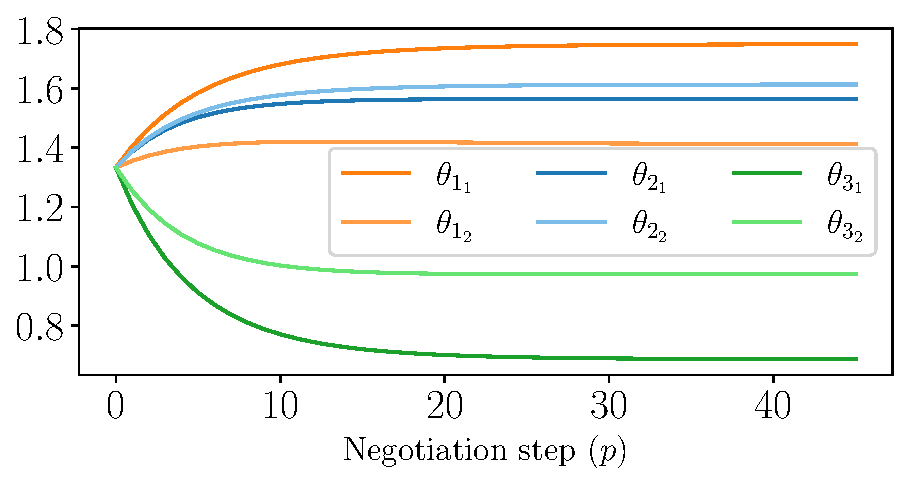
\includegraphics[width=\textwidth]{../img/example_primal_decomposition/example_theta.pdf}
    \caption{Évolution de $\thetai$.}\label{fig:example_theta_fr}
  \end{subfigure}
  \hfill
  \begin{subfigure}{0.45\textwidth}
    \centering
    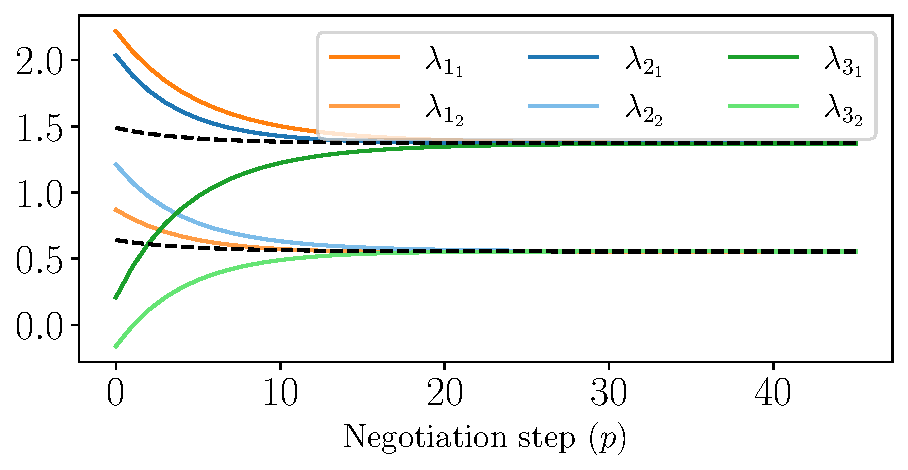
\includegraphics[width=\textwidth]{../img/example_primal_decomposition/example_lambda.pdf}
    \caption{Évolution de $\lambdai$.}\label{fig:example_lambda_fr}
  \end{subfigure}
    \caption{Évolution des variables pendant procès itératif.}\label{fig:example_variables_fr}
\end{figure}

Les valeurs de $\thetai$ représentent une allocation de l'entréé maximale donnée aux agents par le coordinateur, et $\lambdai$ est une mésure de insatisfaction de chaque agent à la valeur allouée.
Le rôle du coordinateur est de négocier les allocations jusqu'à que tous les agenst soient également insatisfaits.
Le procès itératif est appellé la \textbf{phase de négociation}.

À cause de ce procès d'allocations itératives, autres noms sont donés à la décomposition, comme \textbf{allocation des ressources} ou \textbf{décomposition par quantités}.

\subsection{Attack of interest}\label{sec:attack-interest_fr}

Comme les $\lambdai$ sont les sous-gradients des problème locaux~\eqref{eq:DOP_local_fr}, il est possible de voir qu'ils portent de l'information du problème, i.e.\ il y a d'une certaine façon l'information de la $5$-tuple $(H_{i},\vec{f}_{i}[k],\bar{\Gamma}_{i},\thetaik)$, qu'on appelle l'information locale complète $\set{I}_{i}$.
Alors, les attaques en~\cite{VelardeEtAl2018} (montrés en \S\ref{sec:attacks_in_dmpc_fr}) vont réfléchir en modifications du $\lambdai$.

Pour cette raison, nous nous intéressons en attaques du type \fdi{} entre agents qui modifient leur propre $\lambdai$.

On suppose qu'avant chaque négociation, l'attaquant décide une fonction ${\gamma:\R^{c}\times\R\to \R^{c}}$, pour modifier $\lambdai$ avant de l'envoyer au coordinateur.
Pour faciliter l'analyse on suppose la fonction est linéaire comme
\begin{equation}
  \label{eq:linear_attack_fr}
  \lambdaicheat[k]=\gamma(\lambdaik,k)=\Tik\lambdaik.
\end{equation}

On appelle $\Tik$ la matrice de triche.

Cet attaque peut être interprété comme un cas générale du attaque dit selfish ~\cite{VelardeEtAl2018},
où la constante positive qui multiplie la fonction objectif locale est traduite par une matrice de triche diagonale
\begin{equation}
  \label{eq:selfish_attack}
  \Tik=\tau_{i}[k] I_{c}.
\end{equation}

On illustre avec un example d'un système avec $3$ sous agents.
On fait que l'agent $3$ attaque le système avec~\eqref{eq:linear_attack_fr}.
On simule pour scénarios différents.
Pour chaque scénario, agent $3$ utilise un coefficient de triche $\tau_{3}[k]$ distinct.

En Fig.~\ref{fig:example_vary_tau_objective_fr} et~\ref{fig:example_vary_tau_objective_detail_fr}, on accumule les fonctions objectif locales ${\Jiacc=\sum\limits_{k\in\set{K}}\optobji(\optthetai[k])[k]}$
et aussi l'objectif total ${\Jacc=\sum\limits_{i\in\set{M}}J_{i}^{\text{acc}}}$ pour chaque valeur différent de $\tau_{3}$.

Observe (Fig.~\ref{fig:example_vary_tau_objective_detail_fr}) que $\Jacc$ a sa valeur la plus petite quen $\tau_{3}=1$, i.e., quand il n'y a pas de triche.
Quand $\tau_{3}$ augmente, les fonctions objectif de l'attaquant ($\Jiacc[3]$) décroît au même moment que celles des autres augmentent.
L'opposé se passe pour des valeurs de $\tau_{3}$ entre $0$ et $1$.
Dans ce cas l'attaquant détériore sa propre performance, ce qui ne justifie pas tel attaque, sauf dans un scénario de détournement.

\begin{figure}[h]
  \centering
  \begin{subfigure}{0.50\textwidth}
    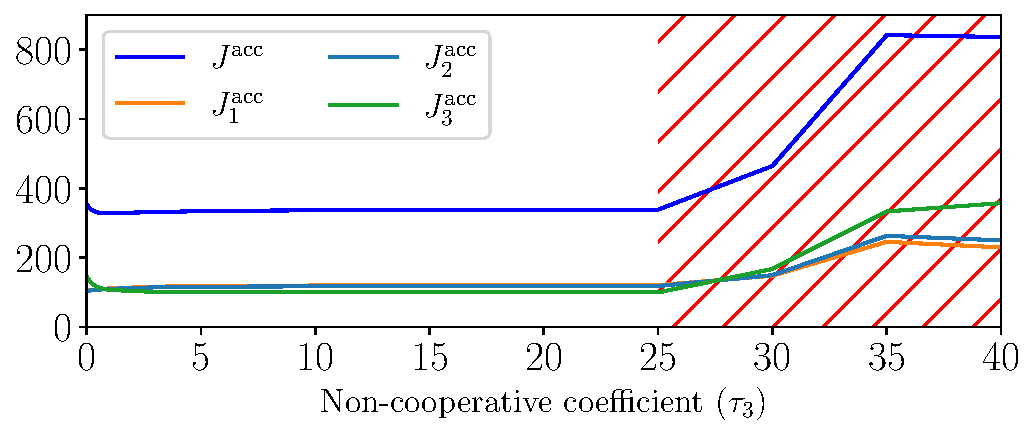
\includegraphics[width=\textwidth]{../img/example_primal_decomposition/example_vary_tau_J.pdf}
    \caption{}\label{fig:example_vary_tau_objective_fr}
  \end{subfigure}
  \begin{subfigure}{0.3\textwidth}
    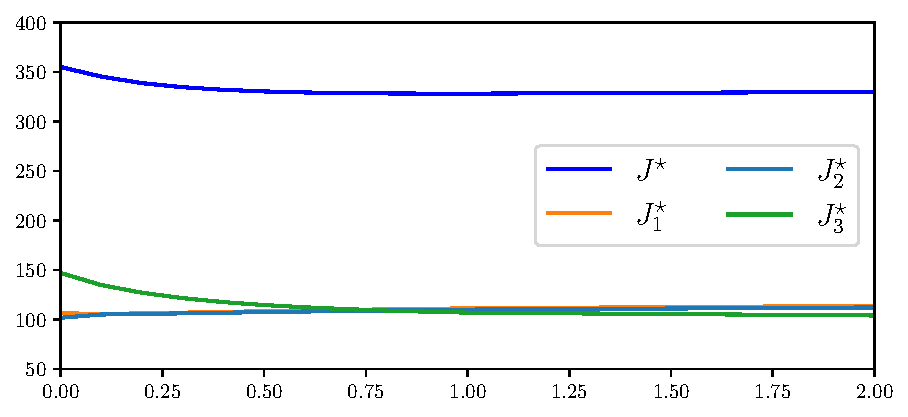
\includegraphics[width=\textwidth]{../img/example_primal_decomposition/example_vary_tau_J_detail.pdf}
    \caption{(detail)}\label{fig:example_vary_tau_objective_detail_fr}
  \end{subfigure}
  \caption{Accumulate objective functions for different values of $\tau_{3}$.}\label{fig:example_vary_tau_objective_both_fr}
\end{figure}

Un autre fait peut être vu dans la zone hachurée en rouge de la Fig.~\ref{fig:example_vary_tau_objective_fr}.
Les fonctions objectif trouvent l'équilibre mais recommencent à augmenter.
Cela est causé par un effondrement de la négociation et les agents n'entrent plus en consensus.
On présente la négociation de $\lambdai$ pour $4$ valeurs différentes de $\tau_{3}$ (Figs.~\ref{fig:example_vary_tau_lambda_fr}).

\begin{figure}[h]
  \centering
  \begin{subfigure}{0.45\textwidth}
    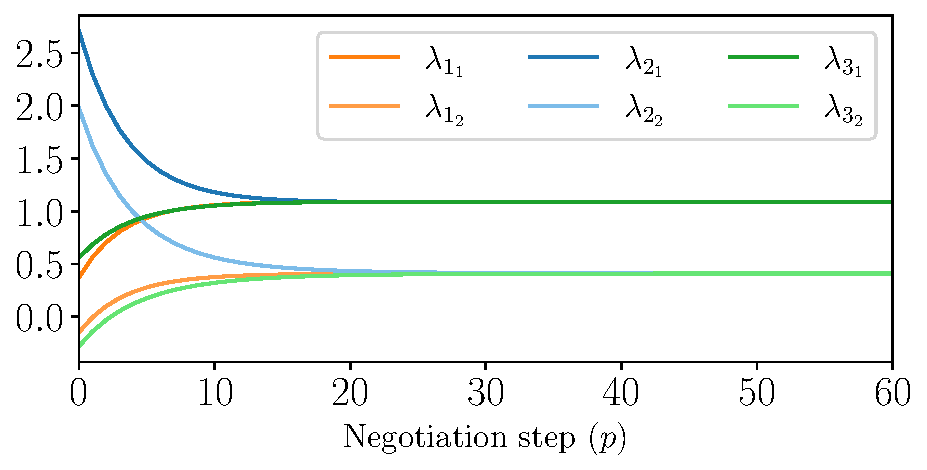
\includegraphics[width=\textwidth]{../img/example_primal_decomposition/example_vary_tau_lambda_tau_1.0.pdf}
    \caption{$\tau_{3}=1$.}\label{fig:example_vary_tau_lambda_tau_1}
  \end{subfigure}
  \begin{subfigure}{0.45\textwidth}
    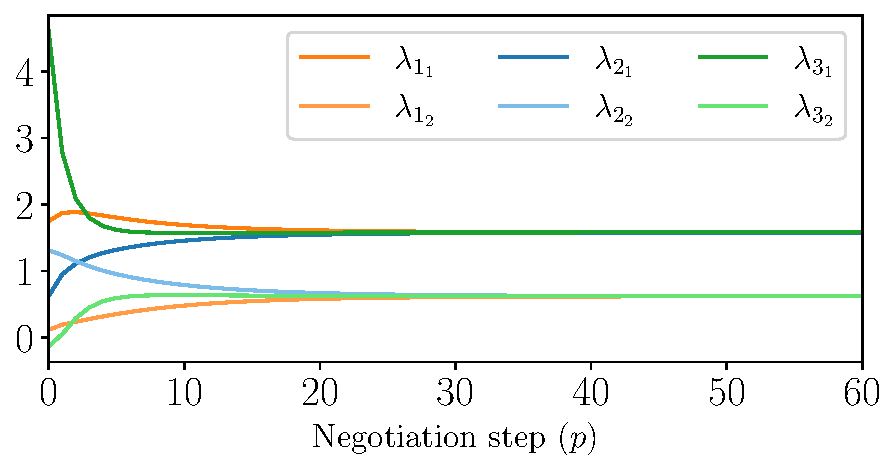
\includegraphics[width=\textwidth]{../img/example_primal_decomposition/example_vary_tau_lambda_tau_5.0.pdf}
    \caption{$\tau_{3}=5$.}\label{fig:example_vary_tau_lambda_tau_5}
  \end{subfigure}
  \\~\\
  \begin{subfigure}{0.45\textwidth}
    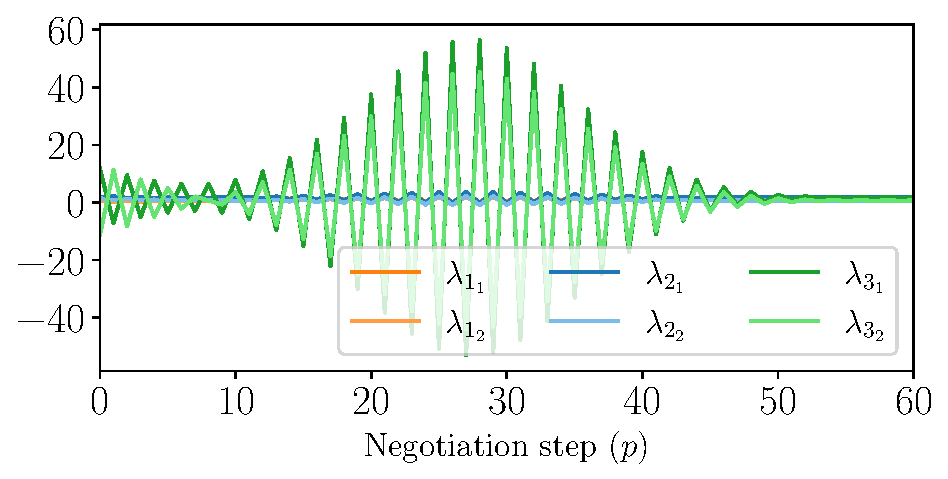
\includegraphics[width=\textwidth]{../img/example_primal_decomposition/example_vary_tau_lambda_tau_20.0.pdf}
    \caption{$\tau_{3}=20$.}\label{fig:example_vary_tau_lambda_tau_20}
  \end{subfigure}
  \begin{subfigure}{0.45\textwidth}
    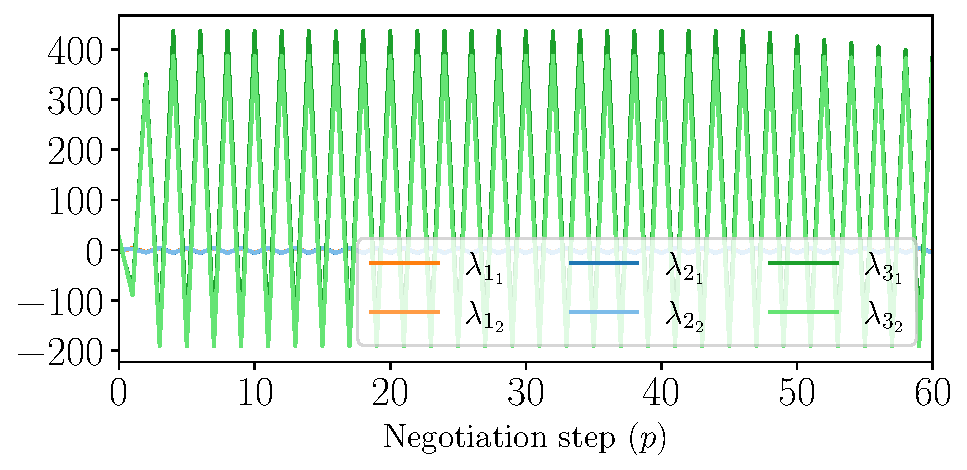
\includegraphics[width=\textwidth]{../img/example_primal_decomposition/example_vary_tau_lambda_tau_40.0.pdf}
    \caption{$\tau_{3}=40$.}\label{fig:example_vary_tau_lambda_tau_40}
  \end{subfigure}
    \caption{Evolution of $\lambdai$ during negotiation for $k=5$ with different values of $\tau_{3}$.}\label{fig:example_vary_tau_lambda_fr}
\end{figure}
Comme on voit, quand $\tau_{3}$ augmente, la négociation présente un comportement oscillatoire atténué.
L'attenuation diminue si $\tau_{3}$ augmente, jusqu'à la négociation oscille et aucun consensus soit achévé, cassant la \dmpc{} et peut être aussi le système.

\newpage
\section{Commande Prédictive résiliente pour systèmes dépourvus}\label{sec:comm-pred-resil}

\subsection{Systèmes dépourvus sous attaque}\label{sec:syst-depo-sous}

Différemment de~\cite{VelardeEtAl2018,MaestreEtAl2021}, notre solution pour la \dmpc{} sécurisée est résiliente basée sur la détection active utilisant des méthodes d'apprentissage et des connaissances analytiques du problème.  which propose robust solutions, we propose a resilient \dmpc{} based on a hybrid of analytical/learning active detection method.
Alors, on commence par analyser le système sous attaque.

\subsection{Systèmes dépourvus}\label{sec:deprived-systems_fr}
Premièrement, on rappelle le problème équivalent de la \mpc{} en forme monolitique~\eqref{eq:qp_standard_form_fr}, reproduit ici par convenience,
\begin{equation}
  \label{eq:qp_standard_form_again_fr}
  \tag{\ref*{eq:qp_standard_form_fr}}
  \begin{aligned}
    \begin{matrix}
      \minimiser\limits_{\vec{U}[k]} &
                                                 \frac{1}{2}\norm{\vec{U}[k]}^{2}_{H} + {\vec{f}[k]}^{T}\vec{U}[k] &\\
      \mathrm{sous} &
                             \bar{\Gamma}\vec{U}[k]\preceq {\vec{U}}_{\text{max}}
    \end{matrix}
  \end{aligned},
\end{equation}
et on rappelle les problèmes locaux~\eqref{eq:DOP_local_fr} de la décomposition primale,

\begin{equation}
  \label{eq:DOP_local_reprise_fr}
  \tag{\ref*{eq:DOP_local_fr}}
  \eqoptobji(\thetaik)[k]=
  \begin{matrix}
    \minimiser\limits_{\vec{U}_{i}[k]}&\frac{1}{2}\norm{\vec{U}_{i}[k]}^{2}_{H_{i}} + {\vec{f}_{i}[k]}^{T}\vec{U}_{i}[k]\\
    \mathrm{sous} & \bar{\Gamma}_{i}\vec{U}_{i}[k] \preceq \thetaik:\lambdaik
  \end{matrix}.
\end{equation}

Les versions sans contraintes de ces problèmes sont
\begin{align}
  \label{eq:qp_standard_form_unconstrained_fr}
  \begin{aligned}
    \begin{matrix}
      \minimiser\limits_{\vec{U}[k]} &
                                                 \frac{1}{2}\norm{\vec{U}[k]}^{2}_{H} + {\vec{f}[k]}^{T}\vec{U}[k] &\\
    \end{matrix},
  \end{aligned}\\
  \label{eq:DOP_local_unconstrained_fr}
  \begin{aligned}
    \begin{matrix}
    \minimiser\limits_{\vec{U}_{i}[k]}&\frac{1}{2}\norm{\vec{U}_{i}[k]}^{2}_{H_{i}} + {\vec{f}_{i}[k]}^{T}\vec{U}_{i}[k]\\
    \end{matrix},
  \end{aligned}
\end{align}
et ses solutions sont analytiques~\cite{BoydVandenberghe2004}
\begin{align}
  \label{eq:qp_standard_form_unconstrained_solution_fr}
  \optuncU=-H^{-1}\vec{f}[k],\\
  \label{eq:DOP_local_unconstrained_solution_fr}
  \optuncUik=-H_{i}^{-1}\vec{f}_{i}[k].
\end{align}

On appelle un système dépourvu quand la solution sans contrainte $\optuncU$ se situe dehors les frontières du polytope formé par les constraintes pour tout $k$, i.e.,
\begin{equation}
\bar{\Gamma}\optuncU\succ {\vec{U}}_{\text{max}}, \forall k.
\end{equation}

De plus, dans cette section, nous supposons que pour tous les sous-systèmes, leur solutions sans contraintes $\optuncUik$ ne respectent pas les contraintes
\begin{equation}
\bar{\Gamma}_{i}\optuncUik\succ \thetaik, \forall i\in\set{M}, \forall k,
\end{equation}
i.e., même si tous les ressources sont allouées pour un seul sous-système, il n'est pas capable d'achever ses besoin.

Ces hypothèses signifient que la solution optimal de chaque problème nécessiterait beaucoup plus de ressources que le disponible ($\vec{U}_{\max}$).
Alors, les solutions de ces \qp{} sont trouvées par la projection pondérée
\footnote{Un problème \qp{} peut être vu comme une projection pondérée, dans laquelle la mésure de l'ensemble est pondérée par $H$ et le point original est décalé utilisant $\vec{f}_i[k]$}
des solutions sans contraintes sur le polytope.
Normalement, le résultat se donne au périmètre du polytope.

En supposant que les contraintes ont au maximum la même quantité de lignes que colonnes\footnote{Cette hypothèse est acceptable une fois que la plupart des contraintes de puissance sont du type somme des puissances, comme $\sum_{i\in\set{M}}\vec{u}_{i}[k]\leq\vec{u}_{\max}$.}, la solution peut être la même que pour un problème avec des contraintes d'égalité\footnote{Dans notre cas, les contraintes forment un cône, il est facilement prouvé géométriquement que le point projeté est l'apex du cône.}
\begin{equation}
  \label{eq:qp_standard_form_equality}
  \begin{aligned}
    \begin{matrix}
      \minimiser\limits_{\vec{U}[k]} &
                                                 \frac{1}{2}\norm{\vec{U}[k]}^{2}_{H} + {\vec{f}[k]}^{T}\vec{U}[k] &\\
      \mathrm{sous} &
                             \bar{\Gamma}\vec{U}[k]= {\vec{U}}_{\text{max}}
    \end{matrix}
  \end{aligned}.
\end{equation}

Si on utilise la décomposition primale on a
\begin{equation}
  \label{eq:example_local_problem_reprise_fr}
   \eqoptobji(\thetaik)[k]= \begin{matrix}
    \minimize\limits_{\vec{U}_{i}[k]}&\frac{1}{2}\norm{\vec{U}_{i}[k]}^{2}_{H_{i}} + {\vec{f}_{i}[k]}^{T}\vec{U}_{i}[k]\\
    \mathrm{subject~ to} & \bar{\Gamma}_{i}\vec{U}_{i}[k] = \thetaik:\lambdaik
  \end{matrix}
\end{equation}
comme problèmes locaux et pour la mise à jour on développe la projection pour une intersection de hyperplans résultant
\begin{equation}
  \label{eq:example_projectedSubgradient_lambda_reprise_fr}
 \thetai\pplusone=\thetai\p+\rho\p\left(\lambdai\p-\frac{1}{M}\sum_{j=1}^{M}\vec{\lambda}_j\p\right),\forall i\in\set{M}.
\end{equation}

Ces équations seront utilisées pour une brève analyse du système sous attaque.
\begin{remark}
  On utilise des systèmes dépourvus, car quand en manque de ressources, les agents doivent faire le compromis.
  Ça instigue la compétition entre eux et éventuellement des comportements égoïstes.
  Si ses besoins étaient achévés, il n'aurait pas de motivation pour une triche, tous les agents seraient satisfaits.
\end{remark}

\subsection{Analysises des problèmes locaux}\label{sec:analysis-local-problems_fr}
Comme les problèmes~\eqref{eq:example_local_problem_reprise_fr} sont des \qp{} avec des contraintes d'égalité, on peut trouver une solution analytique~\cite{BoydVandenberghe2004}.

En se basant sur la dualité Lagrangienne on est capable de trouver aussi une solution analytique pour $\lambdaik$.
En calculant le Lagrangien et quelques gradients pour achever les conditions d'optimalité de \KKT{} on a
\begin{equation}
  \label{eq:lambda_function_theta_fr}
  \lambdaik=-\Plin\thetaik-\sik,
\end{equation}
où $\Plin={(\linearcoefi)}^{-1}$ et $\sik=\Plin\bar{\Gamma}_{i}H_{i}^{-1}\vec{f}_{i}[k]$.

Comme attendu, $\lambdaik$ depend de $\thetaik$.
De plus, à cause de la forme quadratique, la solution est affine.

\begin{remark}
  On peut remarquer, comme dit avant la solution intègre les information de la fonction objectif (présence de $H_{i}$ et $\vec{f}_{i}[k]$), et aussi des constraintes (présence de $\bar{\Gamma}_{i}$ et $\thetaik$).
\end{remark}

\subsection{Analyse de la négociation}\label{sec:analysis-negotiation_fr}
Utilisant~\eqref{eq:example_projectedSubgradient_lambda_reprise_fr} et~\eqref{eq:lambda_function_theta_fr}, on peut observer les dynamiques de $\thetai$ et $\lambdai$ pendant la négociation.
Cette analyse donne des idées pour une méthode future de détection et mitigation.

\subsubsection{Dynamique de $\lambdai$}
Si on substitue~\eqref{eq:example_projectedSubgradient_lambda_reprise_fr} en~\eqref{eq:lambda_function_theta_fr}, on a pour chaque sous-système
\begin{equation}
  \label{eq:lambda_dynamics}
\lambdai\pplusone=-\Plin\left(\thetai\p+\rho\p\left(\lambdai\p-\frac{1}{M}\sum_{j=1}^{M}\vec{\lambda}_j\p\right)\right)-\sik.
\end{equation}

En forme matricielle on a la dynamique complète
\begin{equation}
  \label{eq:negotiation_equation_substituting_organizing_matrix_lambda_fr}
  \vec{\lambda}\pplusone=\mathcal{A}_{\lambda}\vec{\lambda}\p,
\end{equation}
où
\begin{equation}
\mathcal{A}_{\lambda}=\left[
\begin{matrix}
I-\frac{M-1}{M}\rho\p \Plin[1] & \frac{1}{M}\rho\p \Plin[1]&\dots&\frac{1}{M}\rho\p \Plin[1]\\
\frac{1}{M}\rho\p \Plin[2]&I-\frac{M-1}{M}\rho\p \Plin[2]&\dots&\frac{1}{M}\rho\p \Plin[2]\\
\vdots&\vdots&\ddots&\vdots\\
\frac{1}{M}\rho\p \Plin[M]&\frac{1}{M}\rho\p \Plin[M]&\dots&I-\frac{M-1}{M}\rho\p \Plin[M]\\
\end{matrix}
\right].
\end{equation}

On voit que c'est un système à temps discret, en anglais \dt{}, homogène.
Le système varie avec le temps, à cause de $\rho$, mais on peut le choisir de façon qu'il disparaisse quand $p\to\infty$.
Alors, on peu utiliser le critère de Lyapunov~\cite[\S8.6]{Hespanha2009}, i.e., les valeurs propres de $\mathcal{A}_{\lambda}$ doivent être dans le cercle unitaire pour que le système soit stable.
Pour des systèmes petits, on peut utiliser le critère de Jury~\cite{Jury1962} pour vérifier ça.

Analisant $\mathcal{A}_{\lambda}$ encore, on voit que la somme des ses colonnes est égale a un\footnote{$I+\frac{M-1}{M}\rho\p \Plin+\sum\limits_{j=1}^{M-1}\frac{1}{M}\rho\p \Plin=I$},
signifiant que $1$ est une valeur propre par la droite $\mathcal{A}_{\lambda}$:
\begin{equation*}
  \mathcal{A}_{\lambda}\1=\1
\end{equation*}
Alors, si on suppose que les autres valeurs propres sont dedans le cercle unitaire, le système converge à un état $\1c$, i.e., où tous les $\lambdaik$ sont égaux~\cite{GarinSchenato2010,XiaoEtAl2007}.
Par contre, la somme des lignes n'est pas égal, alors la somme des états n'est pa constante, où comme dit dans la communauté des algorithmes de consensus, la masse n'est pas conservée.
De cette façon, on ne pourrait pas utiliser des stratégies de consensus moyen, sauf si tous les systèmes avaient le même $\Plin$, ce qui rendrait le problème extrêmement pas intéressent (la solution serait de diviser les ressources également entre les sous-systèmes).

Si le système est sous attaque, on utilise le modèle~\eqref{eq:linear_attack_fr},
\begin{equation}
  \label{eq:linear_attack_reprise_fr}
  \tag{\ref*{eq:linear_attack_fr}}
  \lambdaicheat[k]=\Tik\lambdaik.
\end{equation}
Comme n'importe quel agent peut être l'attaquant, on suppose tous les agents attaquent simultanément le système résultant en:
\begin{equation}
  \label{eq:negotiation_equation_substituting_organizing_under_attack_fr}
  \tilde{\vec{\lambda}}\pplusone=\tilde{\mathcal{A}}_{\lambda}\tilde{\vec{\lambda}}\p,
\end{equation}
où
\begin{equation}
\tilde{\mathcal{A}}_{\lambda}=\left[
\begin{matrix}
I-\frac{M-1}{M}\rho\p \Tik[1]\Plin[1] & \frac{1}{M}\rho\p \Tik[1]\Plin[1]&\dots&\frac{1}{M}\rho\p \Tik[1]\Plin[1]\\
\frac{1}{M}\rho\p \Tik[2]\Plin[2]&I-\frac{M-1}{M}\rho\p \Tik[2]\Plin[2]&\dots&\frac{1}{M}\rho\p \Tik[2]\Plin[2]\\
\vdots&\vdots&\ddots&\vdots\\
\frac{1}{M}\rho\p \Tik[M]\Plin[M]&\frac{1}{M}\rho\p \Tik[M]\Plin[M]&\dots&I-\frac{M-1}{M}\rho\p \Tik[M]\Plin[M]\\
\end{matrix}
\right],
\end{equation}

Comme on a montré en \S\ref{sec:attack-interest_fr}, les matrices de triche $\Tik$ peuvent change les valeurs propres de la matrice, éventuellement faisant le système osciller et ne pas converger aux valeurs optimales.

\subsubsection{Dynamique de $\thetai$}
Similairement, si on fait le contraire et substitue~\eqref{eq:lambda_function_theta_fr} en~\eqref{eq:example_projectedSubgradient_lambda_reprise_fr},
ça résulte en
\begin{equation}
  \label{eq:negotiation_equation_substituting_fr}
 \thetai\pplusone=\thetai\p+\rho\p\left((-\Plin\thetai\p-\sik)-\frac{1}{M}\sum_{j\in\set{M}}(-\Plin[j]\vec{\theta}_{j}\p-\vec{s}_{j}[k])\right),\forall i\in\set{M}.
\end{equation}
ou en forme matricielle
\begin{equation}
  \label{eq:negotiation_equation_substituting_organizing_matrix_theta_fr}
  \vec{\theta}\pplusone=\mathcal{A}_{\theta}\vec{\theta}\p+\mathcal{\vec{B}}_{\theta}[k],
\end{equation}
où
\begin{equation}
\mathcal{A}_{\theta}=\left[
\begin{matrix}
I-\frac{M-1}{M}\rho\p \Plin[1] & \frac{1}{M}\rho\p \Plin[2]&\dots&\frac{1}{M}\rho\p \Plin[M]\\
\frac{1}{M}\rho\p \Plin[1]&I-\frac{M-1}{M}\rho\p \Plin[2]&\dots&\frac{1}{M}\rho\p \Plin[M]\\
\vdots&\vdots&\ddots&\vdots\\
\frac{1}{M}\rho\p \Plin[1]&\frac{1}{M}\rho\p \Plin[2]&\dots&I-\frac{M-1}{M}\rho\p \Plin[M]\\
\end{matrix}
\right]
\end{equation}
\begin{equation}
\mathcal{\vec{B}}_{\theta}[k]=\left[
\begin{matrix}
-\frac{M-1}{M}\rho\p \vec{s}_{1}[k]+\frac{1}{M}\rho\p \vec{s}_{2}[k]\dots-\frac{1}{M}\rho\p \vec{s}_{M}[k]\\
\frac{1}{M}\rho\p \vec{s}_{1}[k]-\frac{M-1}{M}\rho\p \vec{s}_{2}[k] \dots-\frac{1}{M}\rho\p \vec{s}_{M}[k]\\
\vdots\\
\frac{1}{M}\rho\p \vec{s}_{1}[k]+\frac{1}{M}\rho\p \vec{s}_{2}[k]\dots-\frac{M-1}{M}\rho\p \vec{s}_{M}[k]\\
\end{matrix}
\right],
\end{equation}
qui aussi est un système \dt{}, mais avec une entrée forcée ($\mathcal{\vec{B}}_{\theta}$).

On peut analyser la stabilité de $\mathcal{A}_{\theta}$ exactement comme fait avec $\mathcal{A}_{\lambda}$, c'est-à-dire, les valeurs propres doivent être dans le cercle unitaire.

On analyse aussi la somme de ses lignes et colonnes.
La somme des colonnes est égal à $1$.
Alors, $1$ est une de ces valeurs propres par la gauche:
\begin{equation}
  \label{eq:1}
  \1^{T}\mathcal{A}_{\theta}=\1^{T}
\end{equation}
Comme esperé, le système conserve la masse, i.e., les $\theta_{i}$ respectent la contrainte d'égalité globale.
De cette façon, la dépendence linéaire entre les $\theta_{i}$ est explicite.
Si on analyse les colonnes, on voit que la somme n'est pas $1$.
Alors, comme nous avons constaté, le système converge mais pas nécessairement à un état où tous les $\theta_{i}$ sont égaux.
Cela serait le cas où les $\Plin$ sont égaux.

Comme on voit, les valeurs propres dependent just de $\Plin$ et $\rho\p$.
Comme les $\Plin$ sont des paramètres du système, le designer ne peut que choisir l'évolution de $\rho\p$.

Une fois le $\rho\p$ choisi, la matrice $\mathcal{A}_{\theta}$ évolue toujours de la même manière.
Alors, s'il y a un changement de cette évolution, ça veut dire que le système présente un comportement anormale.

Comme on peut observer, une perturbation en $\Plin$ (changement de la fonction objectif ou contraintes) change les valeurs de $\mathcal{A}_{\theta}$, et par conséquence sa dynamique.
Ce changement peut déstabiliser le système si les valeurs propres sont décalées dehors le cercle unitaire, comme déjà montré en \S\ref{sec:attack-interest_fr}.
Par contre, les perturbations en $\sik$ (modification de la function objectif, contraintes ou état/référence) peuvent change l'état en régime permanent (changement en $\mathcal{\vec{B}}_{\theta}[k]$).

Si on suppose que le système est sous attaque et tous les agents sont suspects on a la dynamique
\begin{equation}
  \label{eq:negotiation_equation_substituting_organizing_tilde_fr}
  \vec{\theta}\pplusone=\tilde{\mathcal{A}}_{\theta}[k]\vec{\theta}\p+\tilde{\mathcal{\vec{B}}}_{\theta}[k]
\end{equation}
où
\begin{equation}
\tilde{\mathcal{A}_{\theta}}[k]=\left[
\begin{matrix}
I-\frac{M-1}{M}\rho\p \Tik[1]\Plin[1] & \frac{1}{M}\rho\p \Tik[2]\Plin[2]&\dots&\frac{1}{M}\rho\p \Tik[M]\Plin[M]\\
\frac{1}{M}\rho\p \Tik[1]\Plin[1]&I-\frac{M-1}{M}\rho\p \Tik[2]\Plin[2]&\dots&\frac{1}{M}\rho\p \Tik[M]\Plin[M]\\
\vdots&\vdots&\ddots&\vdots\\
\frac{1}{M}\rho\p \Tik[1]\Plin[1]&\frac{1}{M}\rho\p \Tik[2]\Plin[2]&\dots&I-\frac{M-1}{M}\rho\p \Tik[M]\Plin[M]\\
\end{matrix}
\right]
\end{equation}
\begin{equation}
\tilde{\mathcal{\vec{B}}}_{\theta}[k]=\left[
\begin{matrix}
-\frac{M-1}{M}\rho\p \Tik[1]\vec{s}_{1}[k]+\frac{1}{M}\rho\p \Tik[2]\vec{s}_{2}[k]\dots-\frac{1}{M}\rho\p \Tik[M]\vec{s}_{M}[k]\\
\frac{1}{M}\rho\p \Tik[1]\vec{s}_{1}[k]-\frac{M-1}{M}\rho\p \Tik[2]\vec{s}_{2}[k] \dots-\frac{1}{M}\rho\p \Tik[M]\vec{s}_{M}[k]\\
\vdots\\
\frac{1}{M}\rho\p \Tik[1]\vec{s}_{1}[k]+\frac{1}{M}\rho\p \Tik[2]\vec{s}_{2}[k]\dots-\frac{M-1}{M}\rho\p \Tik[M]\vec{s}_{M}[k]\\
\end{matrix}
\right]
\end{equation}

Comme dans le cas avec $\mathcal{A}_{\theta}$, en ajustant les $\Tik$, un attaquant peut changer les valeurs propres de $\mathcal{A}_{\lambda}$.
Les matrices de triche $\Tik$ peuvent être aussi ajusté pour pousser la négociation à un nouveau point, mais comme on voit, ça modifie aussi la dynamique do système.
Alors, les ataquants doivent faire le compromis entre leur gourmandise et de ne pas casser la négociation, ce qu'est pire pour tous les agents, incluant les attaquants.

Quelqu'un peut remarquer qu'on pourrait créer un détecteur de comportement anormale en supervisant la matrice $\mathcal{A}_{\theta}$.
Une fois qu'il y a un changement d'une de ses valeurs propres, un comportement anormale est détecté.

Malheureusement, cette méthode nous donne que la détection, mais pas forcément quel agent à causé l'anomalie, ce que serait utile pour un algorithm de mitigation.
D'ailleurs, pour estimer les éléments de $\mathcal{A}_{\theta}$, il nous serait nécessaire estimer $M^{2}{(c)}^{2}$ éléments\footnote{$M^{2}$ blocs de taille ${c}$}.
Exploitant la structure connue de la matrice et des blocs, on pourrait réduire le total au moins $2M{(\frac{c+{c}^{2}}{2})}$ éléments\footnote{($M$ diagonal + $M$ hors diagonal) blocs symmetriques de taille ${c}$ (seulement triangle supérieur)}.

En suite on verra un mécanisme capable de pas seulement détecter les attaques, mais aussi de identifier l'attaquant, et ça en utilisant la moitié des éléments cités.

\subsection{Détection}\label{sec:detection-mechanism_fr}

Utilisant~\eqref{eq:linear_attack_reprise_fr} on peut récrire~\eqref{eq:lambda_function_theta} comme
\begin{equation}
  \label{eq:lambda_function_theta_tilde}
\lambdaicheat[k]=-\Plintilde\thetaik-\tilde{\vec{s}}_{i}[k],
\end{equation}
où $\Plintilde=\Tik\Plin$ et $\tilde{\vec{s}}_{i}[k]=\Tik\sik$.

Une fois que $\Plin$ doit est constant, n'importe quel chagement entre deux négociations est une conséquence d'un comportement anormal, dans ce cas causé par $\Tik$.

Utilisant la relation entre $\thetaik$ et $\lambdaik$, on peut superviser les échanges entre coordinateur et agents, estimant $\Plintildeestimate$ et $\siktildeestimate$ tels que
\begin{equation}
  \lambdaicheat[k]=-\Plintilde\thetaik-\tilde{\vec{s}}_{i}[k],
\end{equation}

Si on a accès à la valeur nominale de $\Plin$\footnote{Donnée ou estimée à partir de données historiques fiables.}, notée $\Plinnominal$, on peut créer une loi de détection pour chaque agent $i$.
En choisissant une borne arbitraire $\epsilon_{\Plin}$, on peut définir l'erreur
\begin{equation}
  E_{i}[k] =\norm{\Plintildeestimate-\Plinnominal}_{F},
\end{equation}
et la fonction de détection $d_{i}$:
\begin{equation}
  d_{i}=\indicator{E_{i}[k]\geq\epsilon_{\Plin}},
\end{equation}
qui détecte un attaque quand la borne est surpassée, i.e., $d_{i}=1$.
\todo{remarque}
\begin{remark}
  Comme montré en Remarque~\ref{rem:bounds_and_error_fr}, le choix de $\epsilon_{\Plin}$ peut influencer le taux de faux positifs.
  La borne doit être supérieure à l'erreur d'estimation pour un scénario sans attaque.
  La propagation des érreurs n'est pas dans le cadre d'étude de cette thèse.
\end{remark}

\begin{remark}
  Si l'estimation ne converge pas, ça veut dire que les rélations ne sont plus linéaires, et alors on pourrait comme ça détecter un comportement anormal.
\end{remark}

Une brève discussion pour l'estimation de $\Plintildeestimate$ suit.

\subsection{Estimation}\label{sec:about-estimation_fr}
On choisie la méthode des moindres carrés récursive, en anglais \RLS{}~\cite{AstroemWittenmark1989}, pour estimer les paramètres.

Dans le \RLS{}, pour estimer un paramètre $\rlsparam$, on utilise un modèle de régression avec entrées et sorties ($\rlssysinput$ et $\rlssysoutput$) qui nous possibilitent de calculer un résidu $\epsilon$.
Ce résidue, allié à un gain $\rlsgain$, est utilisé pour mettre à jour les estimations de $\rlsparam$.
Comme la valeur exacte n'est pas connue on utilise une initialisation et un terme d'oubli $\rlsforget$ pour mettre à jour le gain $\rlsgain$, et naturellement comme dit le nome, oubliant les événements du passé.

On transforme~\eqref{eq:lambda_function_theta_tilde} pour utiliser un modèle comme
\begin{equation}
  \rlssysinput\rlsparam=\rlssysoutput,
\end{equation}
où on vectorise $\Plintildeestimate$ and $\siktildeestimate$ en $\rlsparam$ et change la structure de $\thetai$ pour créer $\rlssysinput$ et $\rlssysoutput$
\begin{equation}
  \rlsparam=\left[
    \begin{matrix}
      \vectorize{\Plintildeestimate}\\
      \siktildeestimate\\
    \end{matrix}
  \right],
\end{equation}
\begin{equation}
  \rlssysinput=\left[
    \begin{matrix}
      \kron{I_{c}}{\thetai\T}&I_{c}\\
    \end{matrix}
  \right].
\end{equation}

Si on veut utiliser le structure symétrique de $\Plintildeestimate$ and on peut estimer juste le triangle supérieur, en réduisant le total d'éléments à ${\frac{c^{2}+3c}{2}}$.


On restructure $\rlsparam$
\begin{equation}
  \rlsparam=\left[
    \begin{matrix}
      \elem[1,1:c]{\Plintildeestimate}\T\\
      \elem[2,2:c]{\Plintildeestimate}\T\\
      \vdots\\
      \elem[c,c]{\Plintildeestimate}\T\\
      \siktildeestimate\\
    \end{matrix}
  \right].
\end{equation}

Cependant, pour $\rlssysinput$, on utilise un algorithme de construction (Algorithme~\ref{alg:struct_symmetric_fr}):
\begin{equation}
  \rlssysinput=\left[
    \begin{matrix}
      \text{\structDataSym}(\thetai) &  I_{c}
    \end{matrix}
  \right].
\end{equation}

\begin{algorithm2e}[h]
  \DontPrintSemicolon%
  \Fn{\structDataSym($\vec{x}$)}{
    $s\gets\card\vec{x}$\;
    \eSi{$s==1$}{
      $Y\gets \vec{x}$\;
    }
    {
      $Y\gets \left[\begin{smallmatrix}
                  \left[\begin{smallmatrix}
                          \vec{x}\T \\
                          \left[\begin{matrix}
                                  \0_{s-1}& \elem[1]{\vec{x}}I_{s-1}
                                \end{matrix} \right]
                        \end{smallmatrix} \right]
                  & \begin{smallmatrix}
                      \0_{\frac{s^{2}-s}{2}}\T \\
                      \text{\structDataSym}(\elem[2:s]{\vec{x}})
                    \end{smallmatrix}
                \end{smallmatrix}\right]$\;
            }
          }
          \caption{Restructuration de forme symétrique.}\label{alg:struct_symmetric_fr}
        \end{algorithm2e}
Pour mieux comprendre on donne un example.
Si $\thetai$ a ${c=3}$ éléments, en appliquant \structDataSym, ça résulte en
\begin{equation}
  \text{\structDataSym}(\theta_i)=
  \left[
  \begin{matrix}
     \elem[1]{\theta_{i}}  &   \elem[2]{\theta_{i}}   &  \elem[3]{\theta_{i}} &    0  &   0  &   0 \\
     0  &   \elem[1]{\theta_{i}}   &  0 &    \elem[2]{\theta_{i}}  &   \elem[3]{\theta_{i}}  &   0 \\
     0  &   0   &  \elem[1]{\theta_{i}} &    0  &   \elem[2]{\theta_{i}}  &   \elem[3]{\theta_{i}}
  \end{matrix}
  \right].
\end{equation}

\begin{remark}
  On ne nécessite pas de $\sik$ pour la estimation, on l'estime quand même car on l'utilisera pour la mitigation.
\end{remark}

On décrit en Algorithme~\ref{alg:update_rls_fr} comme calculer une estimation de $\rlsparam$.

\begin{algorithm2e}[h]
  \DontPrintSemicolon%
  \Entree{Pas $h$, Oubli $\rlsforget$, Estimation $\rlsparam\h$, Gain $\rlsgain\h$, Entrée $\thetai\h$, Sortie $\rlssysoutput\h$}
  \Sortie{Nouvelle estimation $\rlsparam\hplusone$, Nouveau Gain $\rlsgain\hplusone$ }
  $\rlssysinput\gets\left[\text{\structDataSym}(\thetai\h),I_{c}\right]$\;
  Calculate residual $\rlsresidual$: $\rlsresidual\gets \rlssysoutput-\rlssysinput\rlsparam$\;
  Update gain $\rlsgain$: $\rlsgain\hplusone\gets \rlsforget^{-1}\rlsgain\h-\rlsforget^{-2}\rlsgain\h\rlssysinput\T{(I_{c}+\rlsforget^{-1}\rlssysinput\rlsgain\h\rlssysinput\T)}^{-1}\rlssysinput\rlsgain\h$\;
  Calculate new estimate $\rlsparam$: $\rlsparam\hplusone\gets\rlsparam\h+\rlsgain\hplusone\rlssysinput\T\rlsresidual$\;
  \caption{Update of \RLS{} to estimate $\Plintildeestimate$ and $\siktildeestimate$ simultaneously.}\label{alg:update_rls_fr}
\end{algorithm2e}

On pourrait essayer d'utiliser l'estimation pendant la négociation, mais l'agorithme ne marcherait pas.
Le fait que $\lambdai$ dépend de $\thetai$ et vice-versa fait que la négociation se comporte comme un système \dt{} (comme vu en~\S\ref{sec:analysis-negotiation_fr}).
Cette dépendance diminue l'excitation de l'algorithme et comme vu en~\cite{AstroemWittenmark1989}, ça fait que la solution devienne pas unique, une des matrices devienne singulière.
Une façon d'augmenter artificiellement l'excitation est de déconecter les $\thetai$ de la négociation et utiliser un autre type d'entrée.

On a opté d'utiliser un bruit comme entrée une foi que comme vu en~\cite[\S3.4]{AstroemWittenmark1989}, le signal aléatoire a excitation persistent de n'importe quel ordre.

\subsection{Technique de détection Complete }\label{sec:compl-detect-algor_fr}
La détection peut être décrite enfin par l'Algorithme~\ref{alg:detection_rls_fr}.

\begin{algorithm2e}[h]
  \DontPrintSemicolon%
  \Entree{$\Plinnominal$ Nominal, $h_{\max}$, Borne $\epsilon_{\rlsparam}$, Borne $\epsilon_{\Plin}$, }
  \Sortie{Détection $d_{i}$, Estimations de $\Plintildeestimate$ et $\siktildeestimate$}
  $h\gets0$\;
  Initialise $\rlsparam\p$\;
  \Repeter{$\norm{\rlsparam\hplusone-\rlsparam\h}\leq\epsilon_{\rlsparam}$}
  {
    Coordinateur envoie $\thetai\h$ aléatoire à agent $i$ \;
    Sous-système résout~\eqref{eq:DOP_local_fr}, et envoie  $\lambdaikstar(\thetai\p)$ en retour\;
    Coordinateur met à jour l'estimation de $\rlsparam$ avec Algorithme~\ref{alg:update_rls}\;
    \Si{$\ \left[h\geq h_{\max}\right]$}{
      Coordinateut fixe $d_{i}$: $d_{i}\gets 1$\;
      break\;
    }
    $h\gets h+1$\;
  }
  Reconstruit $\Plintildeestimate$ et $\siktildeestimate$ à partir de $\rlsparam$\;
  $E_{i}[k]\gets\norm{\Plintildeestimate-\Plinnominal}_{F}$\;
  Coordinateur calcule $d_{i}$: $d_{i}\gets d_{i}\lor \indicator{E_{i}[k]\geq\epsilon_{\Plin}}$\;

  \caption{Algorithme de détection dans un pas $k$ (en parallèle si possible).}\label{alg:detection_rls_fr}
\end{algorithm2e}

Une fois les attaquants identifiés, on a besoin de la mitigation pour réduire les effets.

\newpage
\subsection{Mitigation}\label{sec:mitigation_fr}
Pour la mitigation on a quelques possibilités d'objectifs.
On donne un petit exemple.

\subsubsection{Exemple Qualitatif}\label{sec:qualitative-example_fr}

Imaginons un système simple de deux sous-systèmes \ltidt{} d'une dimension, contraints par l'entrée, controllés par la \dmpc{} presentée dans ce travail, problèmes du type \qp{} et toute autre condition imposé dans cette section.
On utilise un horizon de prédiction $\predhorz=1$ and contraintes locales $\vec{u}_{i}\geq\0$ pour faciliter la visualisation.

Si on trace les courbes de niveaux du système (Fig.~\ref{fig:original_minimum_fr}), on voit le minimum sans contraintes projeté (projection pondérée) sur le hyperplan.
La projection résulte la solution sous contraintes (point bleu).
\begin{figure}[h]
  \centering
  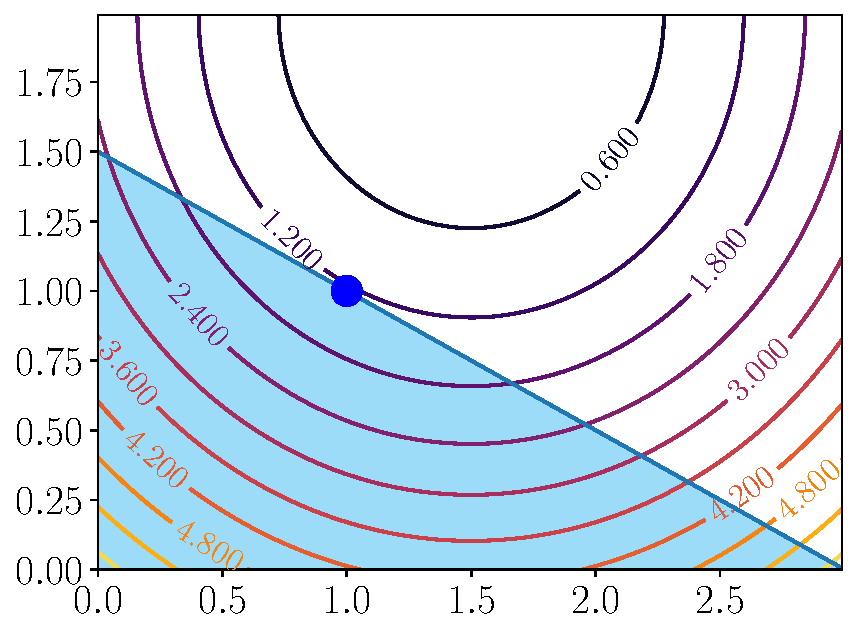
\includegraphics[width=7cm]{../img/resilient_eq/original-minimum.pdf}
  \caption{Minimum Original.}\label{fig:original_minimum_fr}
\end{figure}

Une fois qu'un agent attaque le système~\eqref{eq:linear_attack_reprise_fr}, les courbes sont déformées (Fig.~\ref{fig:minimum_after_attack_fr}).
Cette distortion change la projection, resultant en une nouvelle solution (en vert).
\begin{figure}[h]
  \centering
  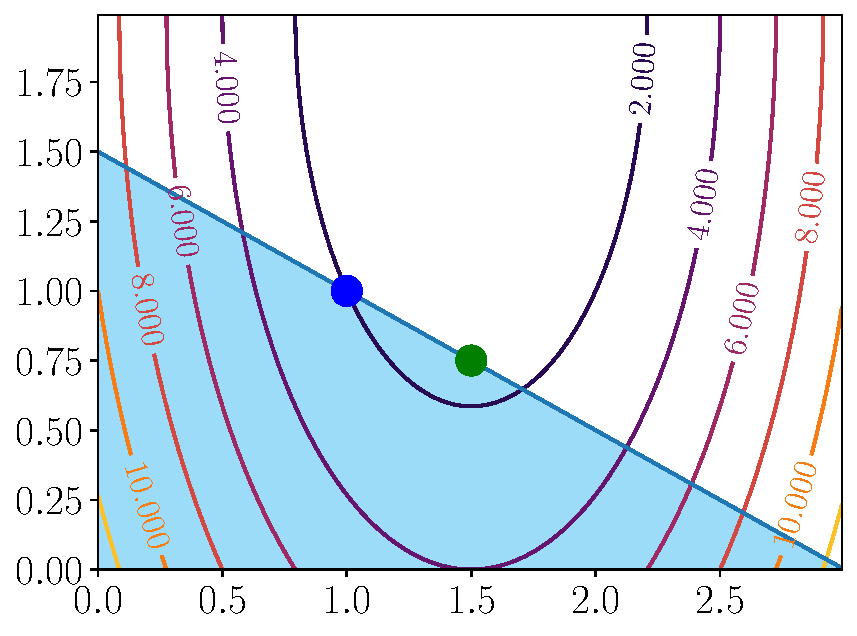
\includegraphics[width=7cm]{../img/resilient_eq/new-minimum-selfish.pdf}
  \caption{Minimum après attaque.}\label{fig:minimum_after_attack_fr}
\end{figure}

Si l'attaquant est détecté, une option est de mitiger la dérive par substituant le $\lambdaicheat$ réçu par $\0$.
Cela peut être interpreté comme un coordinateur punissant l'attaquant, en supposant que l'attaquant est satisfait $\lambdai=\0$, indépendamment de l'allocation faite.
Cette négligence vers l'attaquant résulte en lui recevant moins et moins de ressources.
À la limite, ça serait comme si l'attaquant ne faisait plus part de la négociation, en étant débranché, comme en~\cite{VelardeEtAl2018,MaestreEtAl2021}.

Si on le fait (Fig.~\ref{fig:minimum_ignoring_attacker}) on voit les nouvelles courbes et la nouvelle solution (en orange).
\begin{figure}[h]
  \centering
  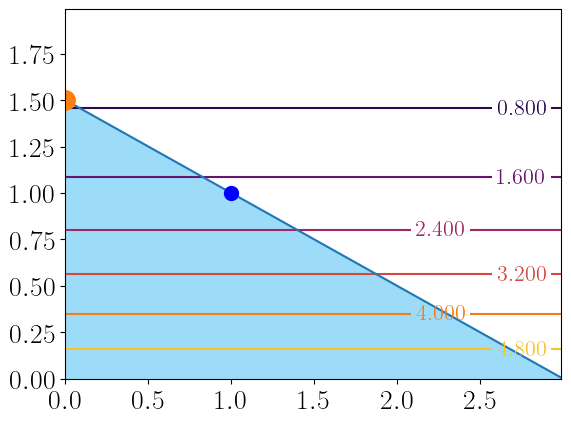
\includegraphics[width=7cm]{../img/resilient_eq/ignoreX.png}
  \caption{Nouveau optimal quand négligent l'attaquant.}\label{fig:minimum_ignoring_attacker_fr}
\end{figure}

Même si l'idée de punir l'attaquant semble attirante, comme nous controllons un \cps{} ça peut affecter la qualité de service, en anglais \QoS{}, et par conséquence les personnes.

Une solution serait d'allouer des ressources suffisantes pour un niveau minimal de \QoS{}, mais ça peut être un peu difficile à cause de sa subjectivité.

Nous proposons une autre solution, essayer de récuperer le comportement normal, tant que quelques hypothèses soient garanties.
Cela permet de passer des courbes du système attaqué (Fig.~\ref{fig:minimum_after_attack_fr}) à des autres, comme montré en Fig.~\ref{fig:minimum_recovered_fr}, où le nouveau minimum s'encontre dans une voisinage acceptable de l'original.

\begin{figure}[h]
  \centering
  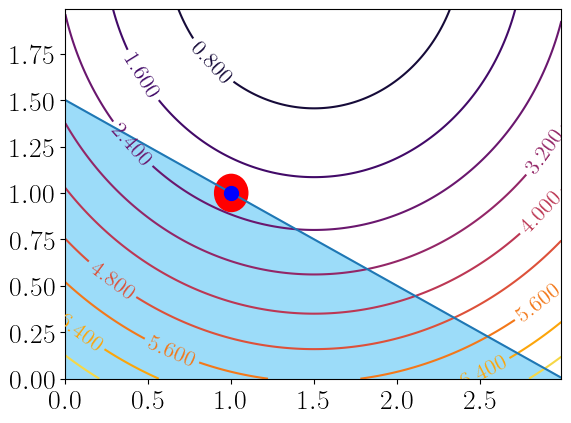
\includegraphics[width=7cm]{../img/resilient_eq/correctX.png}
  \caption{Valeur optimale après récuperer comportement original.}\label{fig:minimum_recovered_fr}
\end{figure}

\subsubsection{Récuperant comportement nominal}\label{sec:recov-nomin-behav_fr}
Comme vu, si $\lambdai=\0$, ça veut dire que l'allocation de l'agent lui satisfait.
Alors, on n'espère pas que l'attaquant va tricher pour dire qu'il est satisfait quand il n'y est pas.

De cette façon, on assume que
\begin{equation}
  \left[\lambdaicheat=\0 \right] \iff \left[\lambdai=\0 \right],
\end{equation}
qui signifie que
\begin{equation}
  \label{eq:T_is_invertible}
  \lambdaicheat=\Tik\lambdai=\0\text{, if and only if }\lambdai=\0,
\end{equation}
impliquant que $\Tik$ est \textbf{inversible}.

En observant~\eqref{eq:lambda_function_theta_tilde_fr}, on suppose aussi que le choix de $\Tik$ ne change pas le structure de $\Plin$, i.e., $\Plintilde$ est aussi symétrique.

Si on a l'estimation $\Plintildeestimate$ et la valeur nominale $\Plinnominal$, avec ces hypothèses on peut estimer l'inverse de $\Tik$:
\begin{equation}
  \label{eq:estimate_T_inverse_fr}
{\Tikinvestimate=\Plinnominal{\Plintildeestimate}^{-1}}.
\end{equation}

Et avec cette estimation on peut reconstruire $\lambdai$:
\begin{equation}
  \label{eq:lambdareconstruction}
  \lambdaireconstructed=-\Plinnominal\thetai-\Tikinvestimate\siktildeestimate
\end{equation}

Alors, on peut moduler la négociation en choisissant la version de $\lambdai$ qu'on veut, i.e.,
\begin{equation}
  \lambdaimodified=
          \begin{cases}
            \lambdaicheat, &\text{if } d_{i}=0\\
            \lambdaireconstructed, &\text{if }d_{i}=1\\
        \end{cases}
\end{equation}

\begin{remark}
  Observe que si l'estimation ne converge pas on ne peut pas réconstruire $\lambdaik$.
  Une solution serait ignorer l'attaquant comme montré.
  Par contre, on ignore les cas où l'estimation ne converge pas.
\end{remark}

\subsection{La dMPC résiliente pour systèmes dépourvus}\label{sec:complete-safe-dmpc_fr}
En mettant ensemble les méthodes de détection et mitigation présentées, on peut finalement avoir notre \dmpc{} résiliente basée sur la décomposition primale pour systèmes dépourvus, ou en anglais \rpdmpcss{}.
On peut observer que les mécanismes présentés peuvent être vus comme un superviseur ajouté pour chaque agent (Fig.~\ref{fig:dmpc_communication_safe_eq_fr}).
Algorithme~\ref{alg:rpdbdmpcss} systematize la méthode.

\begin{figure}[H]
  \centering
  \begin{tikzpicture}[font=\small,thick,node distance=3*0.6180cm and 0.6180cm,every node/.style=rectangle,
    mpcSmall/.style={fill=mpc_agent, minimum height=0.6180*2cm, minimum width=2cm},
    coordinator/.style={fill=mpc_coordinator, minimum height=0.6180*3.5cm, minimum width=6.5cm},
    supervisor/.style={fill=mpc_green, minimum height=0.6180*3*0.3cm, minimum width=2cm},
    ]

    \node[draw, mpcSmall,] (block1) {\small Agent 1};
    \node[fill=none, draw=none, right=of block1,] (mult) {\bf $\dots$};
    \node[draw, mpcSmall, fill=mpc_agent, right=of mult,] (blockM) {\small Agent M};
    \node[draw, coordinator, below=of mult,] (coordinator) {Coordinateur};

    \node[draw, supervisor,anchor=north west] at (coordinator.north west) {\small Superviseur 1};
    \node[draw, supervisor,anchor=north east] at (coordinator.north east) {\small Superviseur M};

    \draw[-latex,line width=1pt] (block1.south)+(0.4,.0) -- ( coordinator.north -| {$(block1.south)+(0.4,.0)$}) node [right,midway] {$\lambda_{1}$};
    \draw[latex-,line width=1pt] (block1.south)+(-0.4,0) -- (  coordinator.north -| {$(block1.south)+(-0.4,0)$}) node [left,midway] {$\theta_{1}$};
    \draw[-latex,line width=1pt] (blockM.south)+(0.4,.0) -- ( coordinator.north -| {$(blockM.south)+(0.4,.0)$}) node [right,midway] {$\lambda_{M}$};
    \draw[latex-,line width=1pt] (blockM.south)+(-0.4,0) -- (  coordinator.north -| {$(blockM.south)+(-0.4,0)$}) node [left,midway] {$\theta_{M}$};
  \end{tikzpicture}
  \caption{Échange entre agents et coordinateur dans la \rpdmpcss{}.}\label{fig:dmpc_communication_safe_eq_fr}
\end{figure}

\begin{algorithm2e}[h]
  \DontPrintSemicolon
  \detectPhasefr{
    Coordinateur compute $d_{i}$ et estimations de $\Plintildeestimate$ avec Algorithme~\ref{alg:detection_rls_fr}\;
  }
  \negotPhasefr{
    $p\gets 0$\;
    Coordinateur initialise $\vec{\theta}^{(p)}$ et les envoie aux sous-systèmes\;
    \Repeter{$\left[\norm{{\vec{\theta}[k]}^{(p)}-{\vec{\theta}[k]}^{(p-1)}}\leq\epsilon\right]\lor \left[p\geq p_{\max}\right]$}{
      Sous-systèmes résout~\eqref{eq:DOP_local_fr}, et envoient $\vec{\lambda}^{\star}_{i}(\vec{\theta}\p)$\;

      Coordinateur m-à-j les allocations~\eqref{eq:example_projectedSubgradient_lambda_reprise_fr} avec versions adéquates de $\vec{\lambda}_{i}$:\;
      \quad$\vec{\lambda}_{i}^{\star}(\vec{\theta}\p)$, si $d_{i}=0$ et $\lambdaireconstructed$, si ${d_{i}=1}$~\eqref{eq:lambdareconstruction}\;
      $p\gets p+1$
    }
    Agents appliquent la dernière commande $\vec{u}_{i}^{\star}[0|k]$ calculée\;
    $k\gets k+1$\;
  }
  \caption{La \dmpc{} Résiliente basée sur la décomposition primale pour systèmes dépourvus.}\label{alg:rpdbdmpcss_fr}
\end{algorithm2e}

\subsection{Expériment Numérique}\label{sec:numerical-experiment_fr}

\subsubsection{Étude de cas}\label{sec:case-study}

Notre étude de cas est un simple \dhn{} composé par ${M=4}$ petites maisons (appelées I, II, II and IV).
Chacune a un état $\vec{x}_{i}$, et une référence de temperature différente $\vec{w}_{i}(t)$ (besoins diveses).
Les maisons sont equipées de convecteurs, et la puissance total de chauffage de chaque maison est l'entrée $\vec{u}_{i}(t)$.
Comme il n'y a pas de dispositifs pour rafraîchir l'ambient, les entrées sont positives, i.e., $\vec{u}_{i}[k]\succeq\0$.
En Fig.~\ref{fig:houses} les maisons consomment la puissance d'un fournisseur.

\begin{figure}[h]
  \centering
  \begin{tikzpicture}[node distance=.5cm and .75cm,scale=1]
    \node[color=mpc_agent] (house1) at (0,0) {\scalebox{2.5}{\faHome}};
    \node[minimum height=1cm,below=of house1] (medium) {};
    \node[color=mpc_agent,right=of medium] (house2)  {\scalebox{3.5}{\faHome}};
    \node[color=mpc_agent,below=of medium] (house3)  {\scalebox{3}{\faHome}};
    \node[color=mpc_agent,left=3cm of medium] (house4)  {\scalebox{7}{\faHome}};

    \draw[latex-,line width=1pt] (house1) -- (medium.center);
    \draw[latex-,line width=1pt] (house2) -- (medium.center);
    \draw[latex-,line width=1pt] (house3) -- (medium.center);
    \draw[latex-,line width=1pt] (house4) -- (medium.center) node[above,midway] {\large $\vec{u}_{i}(t)$};
    \draw[color=black,fill=mpc_coordinator,] (medium) circle [radius=.2cm];

    \node[latex-,line width=7pt] at ($(house4) +(-1,1)$) {\large $w_{i}(t)$};
    \node[latex-,line width=7pt] at ($(house4)$) {$\vec{x}_{i}(t)$};

  \end{tikzpicture}
  \caption{District avec 4 maisons.}\label{fig:houses_fr}
\end{figure}

On modèle des maisons utilisant des modèles 3R-2C monozone ave des fenêtres~\cite{GoudaEtAl2002} (Fig.~\ref{fig:3R2C_model_fr}).
Les paramètres sont décrits sur Tab.~\ref{tab:modelParamMeaning_fr} et~\ref{tab:modelParam_fr}.

\begin{figure}[h]
  \centering
  \begin{circuitikz}[european]
    \draw (0,0) node[tlground]{} to[isource, l=$P^{\text{heat}}$] ++(0,2) to[short, -*] ++(1.5,0) coordinate (a);

    \draw (a) node[above]{$T^{\text{in}}$}  to[C=$C^{\text{air}}$] ++(0,-2) node[tlground]{};
    \draw (0,-3) node[tlground]{} to[isource, l=$I^{\text{sol}}$] ++(0,2)
    to[short, -*] ++(1.5,0) coordinate (b);
    \draw (b) to[C=$C^{\text{walls}}$] ++(0,-2) node[tlground]{};

    \draw (a) -- ++(2,0) coordinate (c) -- ++(0,-.5) to[R=$R^{\text{iw/ia}}$] ++(0,-2) -- ++(0,-.5) coordinate (d);

    \draw (b) node[above]{$T^{\text{walls}}$} to[short,-*] (d);

    \draw (c) --  ++(2.5,0) -- ++(0,-.5) to[R=$R^{\text{oa/ia}}$] ++(0,-2) -- ++(0,-.5) coordinate (e);

    \draw (d) to[R=$R^{\text{ow/oa}}$] (e) to[battery,l=$T^{\text{out}}$] ++(0,-2) node[tlground]{};
  \end{circuitikz}
  \caption{Modèle thermique 3R-2C d'une maison.}\label{fig:3R2C_model_fr}
\end{figure}

\begin{table}[tb]
  \centering
  \caption{Paramètres du Modèle}\label{tab:modelParamMeaning_fr}
  \begin{tabular}[b]{cl}
    \toprule
    Symbole&Signification\\
    \midrule
    $C^{\text{air}}_{i}$  &Capacité termique de l'air intérieur\\
    $C^{\text{walls}}_{i}$ &Capacité termique des parois externes\\
    $R^{\text{iw/ia}}_{i}$ &Resist.\ entre l'air et parois internes\\
    $R^{\text{ow/oa}}_{i}$ &Resist.\ entre l'air et parois externes\\
    $R^{\text{oa/ia}}_{i}$ &Resist.\ entre l'air intérieur et extérieur (à travers des fenêtres)\\
    $P^{\text{heat}}$ &Puissance de chauffage des convecteurs\\
    $I^{\text{sol}}$ &Puissance irradiée par le Soleil\\
    $T^{\text{in}}$ &Temperature moyenne de l'air à l'intérieur\\
    $T^{\text{walls}}$ &Temperature moyenne des parois internes\\
    \bottomrule
  \end{tabular}
\end{table}

\begin{table}[b]
  \centering
  \caption{
    Paramètres pour chaque maison}\label{tab:modelParam_fr}
  \begin{tabular}[t]{cccccc} \toprule
    Élément& I & II & III & IV &Unit\\
    \midrule
    $C^{\text{walls}}$ & $ 8 $ & $ 7 $ & $ 9 $ & $ 6 $ & $ 10^{4}\mathrm{J/K}$\\
$C^{\text{air}}$   & $ 5.0 $ & $ 4.0 $ & $ 4.5 $ & $ 4.7 $ & $ 10^{4}\mathrm{J/K}$\\
$R^{\text{oa/ia}}$ & $ 5 $ & $ 6 $ & $ 4 $ & $ 5 $ & $ 10^{-3}\mathrm{K/W}$\\
$R^{\text{iw/ia}}$ & $ 2.5 $ & $ 2.3 $ & $ 2.0 $ & $ 2.2 $ & $ 10^{-4}\mathrm{K/W}$\\
$R^{\text{ow/oa}}$ & $ 0.5 $ & $ 1.0 $ & $ 0.8 $ & $ 0.9 $ & $ 10^{-4}\mathrm{K/W}$
\\
    \bottomrule
  \end{tabular}
\end{table}

\pagebreak
Le circuit peut être traduit par le modèle d'espace d'état
  \begin{equation}
  \begin{matrix}
    \label{eq:systems_cont_fr}
    \dot{\vec{x}}_{i}(t)  &=&{A_{c}}_{i}\vec{x}_{i}(t) &+& {B_{c}}_{i}\vec{u}_{i}(t)+{D_{c}}_{i}\vec{d}_{i}(t)\\
    \vec{y}_{i}(t)        &=&{C_{c}}_{i}\vec{x}_{i}(t) &&
  \end{matrix},
\end{equation}
où

\begin{equation}
  \label{eq:4_fr}
  \begin{matrix}
    A_{\mathrm{c}_{i}}=\left[
    \begin{matrix}
      -\frac{1}{C^{\text{walls}}_{i}R^{\text{oa/ia}}_{i}}-\frac{1}{C^{\text{walls}}_{i}R^{\text{iw/ia}}_{i}}& \frac{1}{C^{\text{walls}}_{i}R^{\text{iw/ia}}_{i}}\\
      \frac{1}{C^{\text{air}}_{i}R^{\text{iw/ia}}_{i}} &-\frac{1}{C^{\text{air}}_{i}R^{\text{ow/oa}}o_{i}}-\frac{1}{C^{\text{air}}_{i}R^{\text{iw/ia}}_{i}}
    \end{matrix}\right]
                                                         &
      B_{\mathrm{c}_{i}}=\left[\begin{matrix}  \frac{1}{C^{\text{air}}_{i}}\\ 0\end{matrix}\right]\T
  \\\\
    D_{\mathrm{c}_{i}}=\left[
    \begin{matrix}
      0& \frac{1}{C^{\text{air}}_{i}R^{\text{ow/oa}}_{i}}\\
      \frac{1}{C^{\text{air}}_{i}} &\frac{1}{C^{\text{air}}_{i}R^{\text{ow/oa}}}
    \end{matrix}\right]&C_{\mathrm{c}_{i}}=\left[\begin{matrix}1 & 0\end{matrix}\right]

\end{matrix}
\end{equation}

avec
${\vec{x}_{i}(t)=\left[T^{\text{in}}_{i}(t)\ T^{\text{walls}}_{i}(t)\right]\T}$,
${\vec{u}_{i}(t)=P^{\text{heat}}_{i}}$,
${\vec{d}_{i}(t)=\left[I^{\text{sol}}(t)\ T^{\text{out}}(t)\right]\T}$.

Les entrées $\vec{u}_{i}(t)$ sont contraintes par une puissance de chauffage maximale disponibilisée par le founisseur, i.e.,
\begin{equation}
\sum\limits_{i\in\set{M}}\left[\vec{u}_{i}(t)\right]\preceq \vec{u}_{\max}=40\mathrm{kW}.
\end{equation}

\begin{remark}
  On ignore les perturbation causées par le soleil et l'éxterieur, i.e., $\vec{d}_{i}(t)=\0$.
\end{remark}

Comme on utilise la \mpc{}, on discretise le système avec un bloqueur d'ordre zéro et $T_{s}=0.25\mathrm{h}$ comme pas d'échantillonnage, resultant en les $3$-tuples $(A_{i},B_{i},C_{i})$.

\subsubsection{Appliquant le \rpdmpcss{}}
D'abord, on suppose que le système est dépourvu, c'est à dire, ayant des états initiaux $\vec{x}_{i}[0]$, les références $\vec{w}_{i}[k]$ ne peuvent pas être achevées.

On utilise par exemple, les états
${\vec{x}_{\text{I}}[0]=[ \begin{matrix}
  18.3 & 3.\\
\end{matrix} ]\T}$,
${\vec{x}_{\text{II}}[0]=[ \begin{matrix}
  19.6 & 5.9\\
\end{matrix} ]\T}$,
${\vec{x}_{\text{III}}[0]=[ \begin{matrix}
  18.4 & 5.3\\
\end{matrix} ]\T}$,
and
${\vec{x}_{\text{IV}}[0]=[ \begin{matrix}
  17.4 & 5.3\\
\end{matrix} ]\T}$,
et références
${w_{\text{I}}[0]= 20 }$,
${w_{\text{II}}[0]= 20 }$,
${w_{\text{III}}[0]= 20 }$,
and
${w_{\text{IV}}[0]= 20 }$\nolinebreak.
Utilisant les gains
$Q_{i}=10I$,
et
$R_{i}=   I_{2}$,
et en choisissant de contrôler le système avec un horizon de prédiction
$\predhorz=4$,
on structure le problème de la \dmpc{} et le décompose avec la décomposition primale, avec des problèmes locaux
\begin{equation}
  \label{eq:houses_deprived_local_problem_fr}
  \begin{matrix}
    \minimize\limits_{\vec{U}_{i}[k]}&\obji=\frac{1}{2}\norm{\vec{U}_{i}[k]}^{2}_{H_{i}} + {\vec{f}_{i}[k]}^{T}\vec{U}_{i}[k]\\
    \mathrm{subject~ to} & \bar{\Gamma}_{i}\vec{U}_{i}[k] = \thetaik:\lambdaik\\
                                     &\vec{U}_{i}[k]\succeq\0
  \end{matrix}
\end{equation}

et équations de mise à jour~\eqref{eq:example_projectedSubgradient_lambda_reprise_fr}.

\subsubsection{Résultats}\label{sec:results_fr}
On teste l'algorithme avec une simulation dans une période de
$5$
heures, i.e.,
${k\in\{0,5/T_{s}\}}$,
dans quelques scénarios différents:
\begin{enumerate}
  \item Comportement Nominal (dénoté N)
  \item Agent I attaque le système commandé par \dmpc{} standard (dénoté S)\label{it:case_selfish_fr}
  \item Agent I attaque le système commandé par \rpdmpcss{} (dénoté C)\label{it:case_selfish_recovered_fr}
  % \todo{\item Agents I and IV attack system controlled by standard \dmpc{} (denoted as MS)\label{it:case_selfish_multiple}\note{only if a have time to simulate}}
  % \todo{\item Agents I and IV attack system controlled by \rpdmpcss{} (denoted as MC)\label{it:case_selfish_multiple_recovered}\note{only if a have time to simulate}}
\end{enumerate}

L'attaque choisi pour les scénarios~\ref{it:case_selfish_fr} et~\ref{it:case_selfish_recovered_fr},
sont
\begin{align}
  T_{I}=&\begin{cases}
          \left[\begin{smallmatrix}
  4 & 0 & 0 & 0\\
  0 & 4 & 0 & 0\\
  0 & 0 & 4 & 0\\
  0 & 0 & 0 & 4\\
\end{smallmatrix}
\right],&\text{si }k> 5\\
          I_{c},&\text{sinon}
        \end{cases}
  % T_{IV}=\begin{cases}
  %         \todo{4I_{c}\text{, si }k< 6}\\
  %         I_{c}\text{, otherwise}
  %       \end{cases}
.
\end{align}
\pagebreak

Dans Fig.~\ref{fig:response_houseI_3Scenarios_fr}, on compare la temperature de la maison I ($\vec{y}_{I}[k]$) avec sa référence $\vec{w}_{I}[k]$, et après la variable de détection ${E_{I}(k)}$ avec sa borne $\epsilon_{P}=10^{-4}$.

\begin{figure}[h]
  \centering
  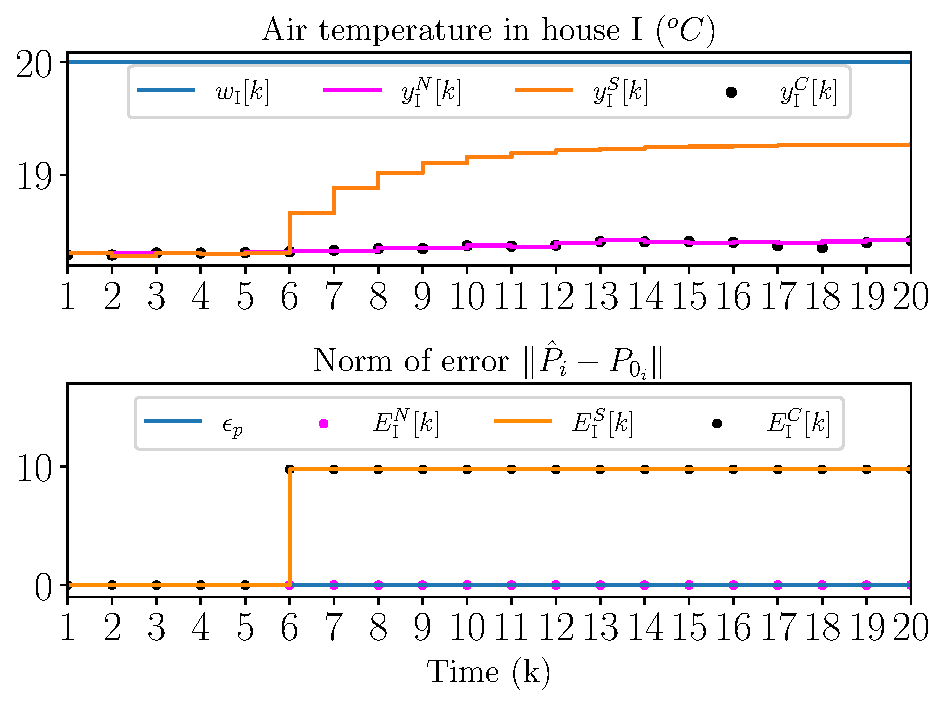
\includegraphics[width=.65\textwidth]{../img/resilient_eq/ErrorWX_command_normErrH.pdf}
\caption{Temperature de la maison I et la variable $E_{I}(k)$ pour les 3 scénarios.}\label{fig:response_houseI_3Scenarios_fr}
\end{figure}
Comme attendu, les variables de détection repose sous la borne $\epsilon_{P}=10^{-4}$ quand on est dans le scénario nominal.
Par contre, pour les scénarios S et C, où l'agent attaque le système, la variable dépasse la borne, indiquant la triche.
En scénario S, on observe l'erreur de suivi ${w_{I}-y_{I}}$ se réduire quand l'attaque est activé, suggérant que l'attaquant pousse la négocitation pour recevoir plus de ressources.
D'ailleurs, les autres agents reçoivent moins de ressources, et leur erreur de suivi augmente (Fig.~\ref{fig:response_housesII_to_IV_3Scenarios_fr}).

Quand la \rpdmpcss{} est activée en scénario C, les temperatures récupèrent un comportement proche du nominal, comme on voit dans Fig.~\ref{fig:response_houseI_3Scenarios_fr} et~\ref{fig:response_housesII_to_IV_3Scenarios_fr}.

% \todo{
%   Similarly, we can show the method works for cases where multiple agents attack the system (Fig.~\ref{fig:response_houses_N_M}),
% \begin{figure}[h]
%   \centering
%   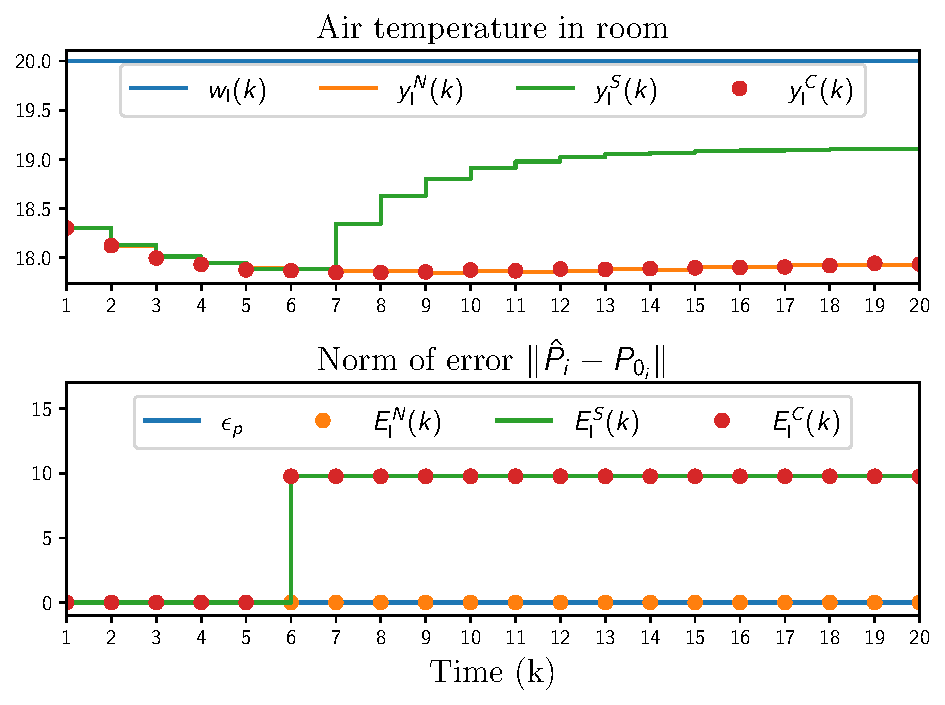
\includegraphics[width=7cm]{AirTempAndDecisionVariable.pdf}
% \caption{Temperature of all houses, and respective references for scenarios N,MS and MC. \todo{remake figure}}\label{fig:response_houses_N_M}
% \end{figure}
% }

On peut aussi comparer les fonctions objectif locales et global $\Jiacc$ et $\Jacc$ dans Tab.~\ref{tab:eq_costsGlobalLocal_fr}.
Comme attendue, la fonction decroît pour l'attaqueur si la \dmpc{} n'est pas sécurisée. Cependant une fois que la \rpdmpcss{} est activé les objectifs reviennent à une valeur proche de l'originale.

\begin{table}[h]
  \centering
  \caption{Fonctions objectif $J_{i}$ (\% erreur)}\label{tab:eq_costsGlobalLocal_fr}
  \begin{tabular}[t]{cccc}
    \toprule
    Agent  & Scénario N& Scénario S & Scénario C\\
    \midrule
    I & $ 299.5 $ & $ 190.8 $ ($ -36.3 $)& $ 301.0 $ ($ 0.0 $)\\
II & $ 192.4 $ & $ 234.1 $ ($ 21.7 $)& $ 191.4 $ ($ -0.5 $)\\
III & $ 305.9 $ & $ 359.1 $ ($ 17.4 $)& $ 305.9 $ ($ -0.0 $)\\
IV & $ 297.5 $ & $ 349.9 $ ($ 17.6 $)& $ 297.2 $ ($ -0.1 $)\\
Global & $ 1095.3 $ & $ 1133.9 $ ($ 3.5 $)& $ 1095.5 $ ($ 0.0 $)
\\
    \bottomrule
  \end{tabular}
\end{table}

\begin{figure}[H]
  \centering
 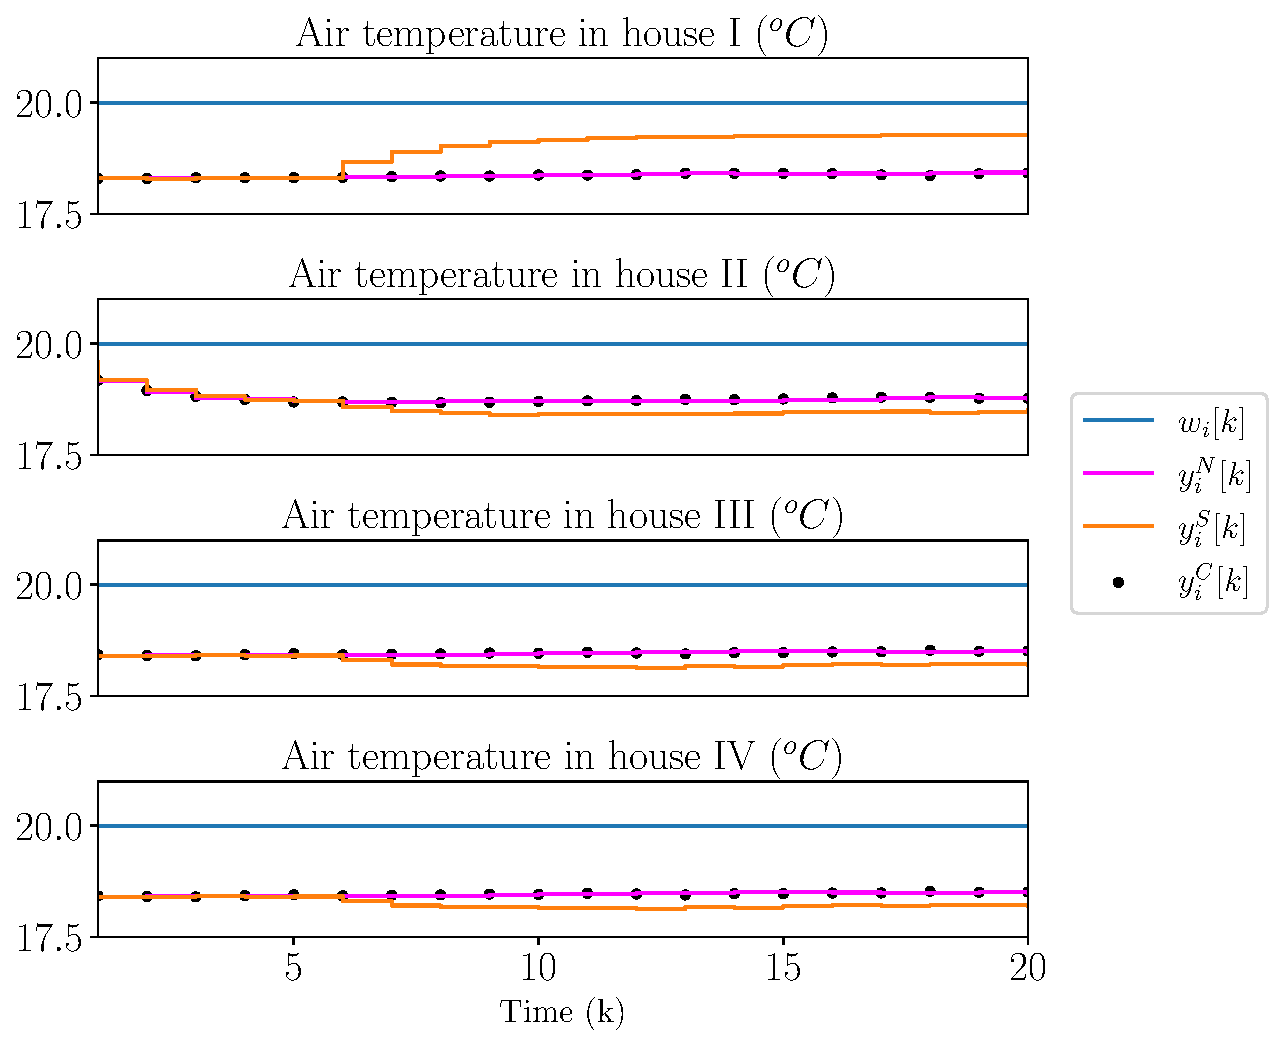
\includegraphics[width=.7\textwidth,trim=0 .3cm 0 .2cm,clip]{../img/resilient_eq/ErrorWX_command_normErrH_all_houses.pdf}
  \caption{Temperature de l'air dans toutes les maisons pour les 3 scénarios.}\label{fig:response_housesII_to_IV_3Scenarios_fr}
\end{figure}

\newpage
\section{Commande Prédictive résiliente sur pénurie artificielle}\label{sec:comm-pred-resil-1}

\subsection{Relaxant le problème}\label{sec:not-so-deprived_fr}
On reprend le problème~\eqref{eq:qp_standard_form_fr} et on ajoute un ensemble de contraintes décomposable $\set{U}$:
\begin{equation}
  \label{eq:qp_standard_form_again_set_constraint_fr}
  \begin{aligned}
    \begin{matrix}
      \minimize\limits_{\vec{U}[k]} &
                                      \frac{1}{2}\norm{\vec{U}[k]}^{2}_{H} + {\vec{f}[k]}^{T}\vec{U}[k] &\\
      \mathrm{subject~ to} & \bar{\Gamma}\vec{U}[k]\preceq {\vec{U}}_{\text{max}} \\
                                    & \vec{U}[k]\in \set{U}
    \end{matrix}
  \end{aligned}.
\end{equation}
On décompose le problème avec la décomposition primale et on a les problèmes locaux:
\begin{equation}
  \label{eq:DOP_local_set_constraint_fr}
  \eqoptobji(\thetaik)[k]=
  \begin{matrix}
    \minimize\limits_{\vec{U}_{i}[k]}&\frac{1}{2}\norm{\vec{U}_{i}[k]}^{2}_{H_{i}} + {\vec{f}_{i}[k]}^{T}\vec{U}_{i}[k]\\
    \mathrm{subject~ to} & \bar{\Gamma}_{i}\vec{U}_{i}[k] \preceq \thetaik:\lambdaik\\
                                     & \vec{U}_{i}[k]\in \set{U}_{i}
  \end{matrix},
\end{equation}
et on résout avec le sous gradient projeté:
\begin{equation}
  \label{eq:projectedSubgradient_lambda_reprise_fr}
  \tag{\ref*{eq:projectedSubgradient_lambda_fr}}
  \vec{\theta}[k]\pplusone=\Proj^{\set{S}}(\vec{\theta}[k]\p+\rho\p\vec{\lambda}[k]\p),
\end{equation}
mais maintenant l'ensemble de la projection est ${\set{S} = \setbuild{\vec{\theta}[k]}{I_{c}^{M}\vec{\theta}[k]\preceq \vec{U}_{\max}}}$.

Dans cette section, on assume encore que la contrainte originale~\eqref{eq:linear_constraint_fr} a au maximum la même quantité de ligne que des colonnes et forment des cônes.
Par contre, on relaxe une hypothèse faite en \S\ref{sec:deprived-systems_fr}.
Les systèmes ne sont plus nécessairement dépourvus, i.e., les solutions sans contraintes
$\optuncU=-H^{-1}\vec{f}[k]$ et $\optuncUik=-H_{i}^{-1}\vec{f}_{i}[k]$ peuvent ou pas respecter les contraintes.

Comme on verra, cette relaxation fait le problème plus générale mais au même moment exponentielment plus complexe.

\subsection{L'impacte sur la solution des problèmes locaux}\label{sec:impact-local-problem_fr}
On peut faire la méme analyse que dans la dernière section.

Même si on a des problèmes \qp{} avec des contraintes d'inégalité, on peut encore utiliser la même méthode Lagrangienne pour trouver une solution analytique.

Par contre, les variables duales qui correspondent aux contraintes d'inégalité doivent être positives~\cite{BoydVandenberghe2004}.
En utilisant les conditions de complémentarité, il est possible de vérifier que $\lambdaik$ est $0$ (ou différent de $0$) dépendant du statuts de chaque contrainte pour la solution sans contrainte $\optuncUik$.

Alors, la solution complète de $\lambdaik$ dépendra de la permutation des statuts des contraintes d'inégalité.
Et si on a $\nineq$ contraintes, on peut avoir potentiellement $2^{\nineq}$ permutations différentes.
\begin{remark}
  On dit potentiellement, car ça peut dépendre de la forme des contraintes, comme on verra en \S\ref{sec:cons-about-stat_fr}.
\end{remark}

On voit que la solution de \eqref{eq:DOP_local_set_constraint_fr} dépend du statut des contraintes, qui dépendent de la valeur de $\thetaik$.
De cette façon, on remarque que l'ensemble des contraintes divise l'espace de $\thetaik$ en plusieurs régions notées $\set{R}_{\lambdai}^{n}$, ou chaque région répresente la combinaison de contraintes actives ou pas pour $\optuncUik$.

Les régions $\set{R}_{\lambdai}^{n}$ sont des polytopes définis par ${\set{R}_{\lambdai}^{n}=\setbuild{\vec{x}}{G^{n}[k]\vec{x} \preceq b^{n}[k]}}$ où les hyperplans peuvent varier avec le temps $k$.
Comme remarqué en~\cite{BemporadEtAl2002}, les polytopes ne se chevauchent pas, i.e., ${\set{R}_{\lambdai}^{i}\cap\set{R}_{\lambdai}^{j}=\emptyset, \forall i\neq j}$.
Alors, les régions forment une partition de l'espace de $\thetai$, i.e., si on a $\thetaik\in\set{Y}\subseteq\R^{c}$, alors ${\bigcup_{i\in\{0:\nineq-1\}}\set{R}^{i}=\set{Y}}$.
\begin{remark}
  La détermination des polytopes n'est pas dans le scope de ce travail, mais peut être trouvé par des méthodes en~\cite[\S4.1.3.2]{LauerBloch2019}.
\end{remark}

Par exemple si on $2$ contraintes l'espace de $\thetai$ pourrait être particioné comme en Fig.~\ref{fig:constraints_partition_theta_fr} (on signalise si les valeurs des variables duales sont égaux à zéro ou pas).
\begin{figure}[h]
  \centering
  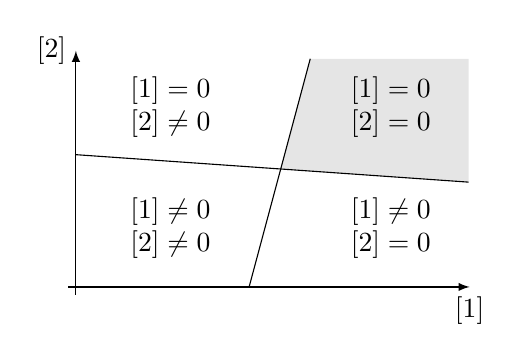
\begin{tikzpicture}[every node/.style={align=center}]
    \def\height{3}
    \def\length{5}
    \node at (0,0) {} coordinate (p0)  ++(0:\length*2.2/5) coordinate (p1) ;
    \node at (0,0) {} ++(90:\height*2.8/5) coordinate (p2) ;

    \draw[black] (p2) ++(-4:5) coordinate (p3);
    \draw[black] (p1) ++(75:3) coordinate (p4);
    \coordinate (p6) at (p3|-p4);

    \coordinate (p5) at (intersection cs:first line={(p2)--(p3)}, second line={(p1)--(p4)});
    \path[fill=gray!20] (p6) -- (p4) -- (p5) -- (p3);
    \draw[black] (p2) -- (p3);
    \draw[black] (p1) -- (p4);

    \draw[-latex] (0,-.1) - - (0,\height) node[left]{$\elem[2]{\thetai}$};
    \draw[-latex] (-.1,0) - - (\length,0) node[below]{$\elem[1]{\thetai}$};

    \node at (\length*1.2/5,\height*1.25/5) {$\elem[1]{\lambdai}\neq0$\\$\elem[2]{\lambdai}\neq0$};
    \node at (\length*1.2/5,\height*3.8/5) {$\elem[1]{\lambdai}=0$\\$\elem[2]{\lambdai}\neq0$};
    \node at (\length*4/5,\height*1.25/5) {$\elem[1]{\lambdai}\neq0$\\$\elem[2]{\lambdai}=0$};
    \node at (\length*4/5,\height*3.8/5) {$\elem[1]{\lambdai}=0$\\$\elem[2]{\lambdai}=0$};
  \end{tikzpicture}
  \caption{Deux contraintes qui partionnent l'espace de $\thetai$.}\label{fig:constraints_partition_theta_fr}
\end{figure}

Pour n'importe quel $\thetai$ dans l'aire grise (l'intersection des hyperplans), la solution de~\eqref{eq:DOP_local_set_constraint_fr} est sans contrainte, i.e., les contraintes seront actives.
Et alors, par définition, le $\lambdai=\0$.
Pour les autres cas, au moins une des contraintes sera inactive, et on peut enlever les actives.
Si toutes les contraintes sont inactives, le résultat est le même que pour le systèmes dépourvus~\eqref{eq:lambda_function_theta_fr}:
\begin{equation}
  \label{eq:lambda_function_theta_reprise_fr}
  \tag{\ref*{eq:lambda_function_theta_fr}}
  \lambdaik=-\Plin\thetaik-\sik,
\end{equation}
\newcommand{\Plinineqnonzero}[1][\star]{\overset{#1}{\Plin}}
\newcommand{\sikineqnonzero}[1][\star]{\overset{#1}{\vec{s}_{i}}[k]}

Si on enleve un ensemble de contraintes, on peut résoudre un problème similaire mais avec un nombre réduit de variables.
Par exemple, si on suppose que la première contrainte est active.
On fait que $\elem[1]{\lambdai}=0$ et on le met à côté, on enlève les lignes correspondant en $\bar{\Gamma}_{i}$ et $\thetai$, et après on résout pour les éléments restant de $\lambdai$. Le résultat est
\begin{equation}
  \label{eq:lambda_function_theta_some_active_fr}
  \elem[2:\elemend]{\lambdai}[k]=-\Plinineqnonzero[2:c] \elem[2:\elemend]{\thetai}[k]-\sikineqnonzero[2:c],
\end{equation}
où $\Plinineqnonzero[2:c]={(\linearcoefiineqnonzero[2:\elemend,\star])}^{-1}$ et $\sikineqnonzero[2:c]=\Plinineqnonzero[2:c]\elem[2:\elemend,\star]{\bar{\Gamma}_{i}}H_{i}^{-1}\vec{f}_{i}[k]$.

On peut faire pareil pour toute autre partition, c'est à dire, toutes les permutations possibles de contraintes actives et inactives.
Ce résultat est la base pour calculer la solution du problème primal utilisé en~\cite{BemporadEtAl2002,AlessioBemporad2009}, qui est la base de la commande \mpc{} explicite.

Cependant, les équations auront de tailles d'éléments différentes (autant d'éléments que de contraintes inactives).
Pour égaliser la taille des équations, on récupere les éléments de $\lambdai$ mises à zéro et mises à côté.
Si on réprend l'exemple,~\eqref{eq:lambda_function_theta_some_active_fr} serait récrite comme
\begin{equation}
  \label{eq:lambda_function_theta_some_active_same_size_fr}
  \lambdaik=
  \left[
    \begin{matrix}
      0\\
      \elem[2:\elemend]{\lambdai}[k]
    \end{matrix}
  \right]
  =
  -
  \left[
    \begin{matrix}
      0&0\\
      0&\Plinineqnonzero[2:c]
    \end{matrix}
  \right]
  \thetaik
  -
  \left[
    \begin{matrix}
      0\\
      \sikineqnonzero[2:c]
    \end{matrix}
  \right]
\end{equation}

Afin de faciliter, on utilise une représentation binaire tel que si on a $\nineq$ contraintes, on utilise $\nineq$ chiffres binaires pour les représenter.
On marque $1$ si la contrainte est active et $0$ sinon.

Dans la Fig.~\ref{fig:constraints_partition_theta_fr}, ${00}_{(2)}$ représente le quadrant inférieur gauche, ${01}_{(2)}$ et ${10}_{(2)}$ les quadrant inférieur droit et supérieur gauche, respectivement, et ${11}_{(2)}$ l'aire en gris.
On utilise la base 10 pour codifier le chiffre.
Alors~\eqref{eq:lambda_function_theta_some_active_same_size_fr} est récrit comme
\begin{equation}
  \label{eq:lambda_function_theta_same_size_coded}
  \lambdaik=-\Plin^{(2^{n_{\text{ineq}-1}})}\thetaik-\sik^{(2^{n_{\text{ineq}-1}})},
\end{equation}
ou l'index $(2^{n_{\text{ineq}-1}})$ indique que juste la première contrainte est active.

On peut alors, écrire la solution complète comme une fonction affine par morceaux, ou en anglais
\pwa{} function:
\begin{equation}
  \label{eq:lambdafuntheta_fr}
  \begin{aligned}
    \lambdaik=
    \begin{cases}
      -\Plinineq\thetaik-\sikineq,&\text{si}\ \thetaik \in\set{R}_{\lambdai}^{n}\\
      \qquad\quad \vdots&\qquad\quad \vdots\\
      -\Plinineq[i][2^{\nineq}-1]\thetaik-\sikineq[i][2^{\nineq}-1],&\text{si}\ \thetaik \in\set{R}_{\lambdai}^{2^{\nineq}-1}\\
    \end{cases}
  \end{aligned}.
\end{equation}

Avec cette équation on peut envisager le changement causé par la relaxation, où on avait juse une équation liant $\lambdai$ à $\thetai$, maintenant on a potentiellement $2^{\nineq}$ équations différentes.

\begin{remark}\label{rem:sparse_solutions_fr}
  Comme attendu, par définition, $\Plinineq[i][n]$ et $\sikineq[i][n]$ sont de plus en plus creuses.
  Quand $n$ augmente, plus en plus contraintes deviennent active, et plus de blocs sont mises à zéro et finalement on a $\Plinineq[i][2^{\nineq}-1]=0_{c}$ et $\sikineq[i][2^{\nineq}-1]=\0_{c}$.
\end{remark}

\subsubsection{Considérations sur le statut des contraintes}\label{sec:cons-about-stat_fr}
Il est important de constater que, comme dit, pour quelques ensembles de contraintes le numéro de permutations n'est pas forcément $2^{\nineq}$.

On donne quelques examples.
Il y a des cas où il n'existe pas une région où toutes les contraintes sont actives, i.e., l'intersection des demi-espaces est nulle (voir Fig.~\ref{fig:non_feasible_fr}).
Ces problèmes sont appelés infaisable, et alors sont ignorés dans ce travail.

\begin{figure}[H]
  \centering
  \begin{tikzpicture}
    \def\ang{-35}
    \def\vecmag{.25}
    \node at (0,0) {} coordinate(p1) ++(\ang:2.5) coordinate(p2) ++(\ang-90:1.5) coordinate(p3) ++(\ang-180:2.5) coordinate(p4);

    \path (p1) -- (p2) coordinate[pos=-0.2](a1l) coordinate[pos=1.2](a1r) coordinate[pos=0.8](m12);
    \draw[-latex] (a1l) -- (m12) -- ([turn] -90:0.5) node[left]{$\vec{\eta}_1$};
    \draw  (m12) -- (a1r);

    \path (p3) -- (p4) coordinate[pos=-0.2](a3l) coordinate[pos=1.2](a3r) coordinate[pos=0.8](m34);
    \draw[-latex] (a3l) -- (m34) -- ([turn] -90:0.5) node[right]{$\vec{\eta}_2$};
    \draw  (m34) -- (a3r);

  \end{tikzpicture}
  \caption{Ensemble de contraintes avec intersection nulle.}\label{fig:non_feasible_fr}
\end{figure}

Dans autres cas, il n'y a pas de région où toutes les contraintes sont inactives.

Par exemple, pour des contraintes avec vecteurs normaux $\vec{\vec{\eta}}_{i}$, si l'angle des demi-espaces $\vecangle{\vec{\eta}_{i}}{\vec{\eta}_{j}}$ est $180^{o}$ et l'intersection n'est pas nulle (voir Fig.~\ref{fig:parallel_only_one_active_fr}), au moins une des contraintes sera toujour active.
\begin{figure}[H]
  \centering
  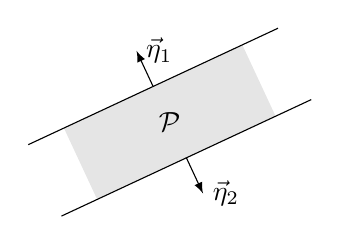
\begin{tikzpicture}
    \def\ang{25}
    \def\vecmag{.5}
    \node at (0,0) {} coordinate(p1) ++(\ang:2.5) coordinate(p2) ++(\ang-90:1.) coordinate(p3) ++(\ang-180:2.5) coordinate(p4);
    \path[fill=gray!20] (p1) -- (p2) -- (p3) -- (p4);
    \node at (barycentric cs:p1=1,p2=1,p3=1,p4=1) {$\mathcal{P}$};

    \path (p1) -- (p2) coordinate[pos=-0.2](a1l) coordinate[pos=1.2](a1r) coordinate[pos=0.5](m12);
    \draw[-latex] (a1l) -- (m12) -- ([turn] 90:0.5) node[right]{$\vec{\eta}_1$};
    \draw  (m12) -- (a1r);

    \path (p3) -- (p4) coordinate[pos=-0.2](a3l) coordinate[pos=1.2](a3r) coordinate[pos=0.5](m34);
    \draw[-latex] (a3l) -- (m34) -- ([turn] 90:0.5) node[right]{$\vec{\eta}_2$};
    \draw  (m34) -- (a3r);
  \end{tikzpicture}
  \caption{Deux contraintes où $\vecangle{\vec{\eta}_{1}}{\vec{\eta}_{2}}=180^{o}$.}\label{fig:parallel_only_one_active_fr}
\end{figure}

Encore autre exemple c'est quand les contraintes forment un polyèdre.
On présent l'exemple minimal, le simplex en $\R^{2}$ (voir Fig.~\ref{fig:triangle_inequality_fr}).
Dans ce cas, on aura toujours au moins $2$ contraintes actives.
\begin{figure}[h]
  \centering
  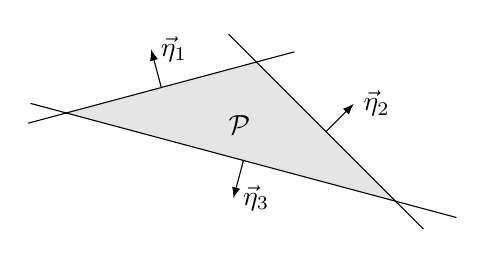
\begin{tikzpicture}
    \node at (0,0) {} coordinate(p1) ++(15:2.5) coordinate(p2) ++(-45:2.5) coordinate(p3) ++ (-195:4.0) coordinate(p4);
    \path[fill=gray!20] (p1) -- (p2) -- (p3);
    \node at (barycentric cs:p1=1,p2=1,p3=1) {$\mathcal{P}$};

    \foreach \X [count=\Y] in {2,...,4}
    {
      \path (p\Y) -- (p\X) coordinate[pos=-0.2](a\Y{}l) coordinate[pos=1.2](a\Y{}r) coordinate[pos=0.5](m\Y\X);
      \draw[-latex] (a\Y{}l) -- (m\Y\X) -- ([turn]90:.5) node[right]{$\vec{\eta}_\Y$};
      \draw (m\Y\X) -- (a\Y{}r);
    }
  \end{tikzpicture}
  \caption{Un polyèdre de $3$ faces.}\label{fig:triangle_inequality_fr}
\end{figure}

Comme on suppose d'avoir au plus la même quantité de contraintes que de dimensions, il n'est possible de créer de polyèdres\footnote{Pour $\R^{n}$, le simplex a $n+1$ faces}. Par contre, pour dimensions supérieures, les prismes doivent aussi être pris en compte.

\subsection{L'impact sur la négociation}\label{sec:impact-local-problem_fr}
On utilise la même techniques qu'en \S\ref{sec:analysis-negotiation_fr}, de substituer une équation dans l'autre.
Ainsi on contemplera la vraie complexité du problème.

La première difficulté est la méthode du sous gradient projeté.
À cause de $\set{S}$ être formé par l'intersection de demi-espaces, la solution est trouvée par la défintion de la projection euclidienne, qui est aussi un problème \qp{}

\begin{equation}
  \label{eq:projected_subgradient_qp}
  \Proj^{\set{S}}(\vec{\theta}[k]\p+\rho\p\vec{\lambda}[k]\p)=
  \argmin\limits_{\vec{x}}
  \left\{
    \begin{matrix}
      \minimiser\limits_{\vec{U}[k]} &
                                      \norm{\vec{x}-\vec{\theta}[k]\p+\rho\p\vec{\lambda}[k]\p}\\
      \mathrm{sous} & I_{c}^{M}\vec{x}\preceq \vec{U}_{\max}:\vec{\mu}\\
    \end{matrix}
  \right\},
\end{equation}
avec sa propre variable duale $\vec{\mu}$.
Pour faciliter la notation on utilise $\vec{x}_{0}=\vec{\theta}[k]\p+\rho\p\vec{\lambda}[k]\p$.

La solution est faite comme en \S\ref{sec:impact-local-problem_fr}.
Et par conséquence la solution a la même forme \pwa{} que~\eqref{eq:lambdafuntheta_fr}:

\begin{equation}
  \label{eq:projection_result_zones_fr}
  \begin{aligned}
    \vec{\theta}[k]\pplusone=
    \begin{cases}
      \vec{x}_{0}+
      {I_{c}^{M}}^{(0)}\left[-P_{\vec{\mu}}^{(0)}\vec{U}_{max}+\vec{s}_{\vec{\mu}}^{(0)}[k]\right],&\text{si}\ \vec{x}_{0}\in\set{R}_{\vec{\mu}}^{0}\\
      \qquad\quad \vdots&\qquad\quad \vdots\\
      \vec{x}_{0},&\text{si}\ \vec{x}_{0}\in\set{R}_{\vec{\mu}}^{2^{c}-1}\\
    \end{cases}
  \end{aligned},
\end{equation}
avec des régions ${\set{R}_{\vec{\mu}}^{n}=\setbuild{\vec{x}}{G_{\vec{\mu}}^{n}[k]\vec{x} \preceq \vec{U}_{\max}^{n}[k]}}$\footnote{Also not defined in this work} qui ne se chevauchent pas, formant une particion de l'espace $\vec{x}_{0}$.
Les élément non creux (codés par les $0$ dans la représentation binaire de $(n)$) de $P_{\vec{\mu}}^{(n)}$ sont ${({I_{c}^{M}}^{(n)}{{I_{c}^{M}}^{(n)}}\T)}^{-1}$, et ces de $\vec{s}_{\vec{\mu}}^{(n)}[k]$ sont ${{({I_{c}^{M}}^{(n)}{{I_{c}^{M}}^{(n)}}\T)}^{-1}{I_{c}^{M}}^{(n)}\vec{x}_{0}}$, ${I_{c}^{M}}^{(n)}$ est construite par l'enlèvement des contraintes comme codées par $(n)$.

Pour $n=0$, la solution est la même que pour le cas d'égalité~\eqref{eq:example_projectedSubgradient_lambda_reprise_fr} ($\card{I_{c}^{M}}=c\times Mc$).
Quand $n=2^{c}-1$ (toutes contraintes sont actives), la solution est la même du cas sans contraintes, une fois que $\vec{\mu}=\0$ (voir Remarque~\ref{rem:sparse_solutions_fr}).

Alors, dépendant de dans quel partition $\vec{\theta}[k]\p+\rho\p\vec{\lambda}[k]\p$ est,
$\thetaik\pplusone$ peut avoir une valeur différent, alors on peut avoir au maximum $2^{c}$ possibilities.
Et $\vec{\theta}[k]\p+\rho\p\vec{\lambda}[k]\p$ depend de $\lambdaik$, qui peut avoir $2^{\nineq}$ modes différents.

Si en \S\ref{sec:analysis-negotiation_fr}, quand on a fait la substitution nous avons trouvé l'expressions des système \dt{}, si on substitue lésultats en~\eqref{eq:projection_result_zones_fr} on aura des systèmes \dt{} hybrides.
Un avec une entrée constante pour $\thetaik$, et un autre homogène pour $\lambdaik$.

Si on conclue le calcules on peut estimer une borne supérieure du nombre total de permutation $\bar{\epsilon}$. Ça totalise
\begin{equation}
  \label{eq:1_fr}
  \bar{\epsilon}=\overbrace{2^{c}}^{\text{régions de la projection}}\times \underbrace{2^{\nineq}\times \dots \times 2^{{\nineq}}}_{M\times \text{régions pour chaque }\lambdai }=2^{c+M\nineq}.
\end{equation}

\begin{remark}
  Problablement quelques contraintes ne sont pas possible, mais encore on voit la croissance exponentiel de nombre de modes du système hybride.
  Le calcul exact n'est pas dans le scope de ce travail.
\end{remark}

Pour le cas dépourvu de la section antérieure, on utilise le cas $(0)$, où $\vec{\theta}[k]\p+\rho\p\vec{\lambda}[k]\p$ est projeté dans l'intersection des tout les demi-espaces.
Et du l'autre hypothèse ($\bar{\Gamma}_{i}\optuncUik\succ \thetaik, \forall i\in\set{M}, \forall k$), on fixe tous les $\lambdai$ à la première solution de~\eqref{eq:lambdafuntheta_fr}.
Les choix consécutifs d'hypothèse réduit le nombre total de modes à un, presenté par~\eqref{eq:negotiation_equation_substituting_organizing_matrix_lambda_fr} et~\eqref{eq:negotiation_equation_substituting_organizing_matrix_theta_fr}:

\begin{equation}
  \label{eq:negotiation_equation_substituting_organizing_matrix_lambda_reprise_fr}
  \tag{\ref*{eq:negotiation_equation_substituting_organizing_matrix_lambda_fr}}
  \vec{\lambda}\pplusone=\mathcal{A}_{\lambda}\vec{\lambda}\p,
\end{equation}
\begin{equation}
  \label{eq:negotiation_equation_substituting_organizing_matrix_theta_reprise_fr}
  \tag{\ref*{eq:negotiation_equation_substituting_organizing_matrix_theta_fr}}
  \vec{\theta}\pplusone=\mathcal{A}_{\theta}\vec{\theta}\p+\mathcal{\vec{B}}_{\theta}[k]
\end{equation}

Si on concatene les répresentations pour la projection et pour chaque problème local, on aura un numéro avec $c+M\nineq$ chiffres.
Et alors, la solution en~\eqref{eq:negotiation_equation_substituting_organizing_matrix_lambda_fr} et~\eqref{eq:negotiation_equation_substituting_organizing_matrix_theta_fr} peut être vu comme le cas spécifique de:
\begin{equation}
  \label{eq:negotiation_equation_substituting_organizing_matrix_lambda_switched_fr}
  \vec{\lambda}[k]\pplusone=
  \begin{cases}
    \mathcal{A}_{\lambda}^{0}\vec{\lambda}[k]\p,&\text{si}\ \vec{\theta} \in \set{R}_{\vec{\lambda}}^{0}\\
    \quad\vdots&\quad\vdots\\
    \mathcal{A}_{\lambda}^{N_{\vec{\lambda}}}\vec{\lambda}[k]\p,&\text{si}\ \vec{\theta}\in\set{R}_{\vec{\lambda}}^{0}\\
  \end{cases}
\end{equation}
\begin{equation}
  \label{eq:negotiation_equation_substituting_organizing_matrix_theta_switched_fr}
  \vec{\theta}[k]\pplusone=
  \begin{cases}
    \mathcal{A}_{\theta}^{0}\vec{\theta}[k]\p+\mathcal{\vec{B}}_{\theta}^{0}[k],&\text{si}\ \vec{\theta}\in\set{R}_{\vec{\theta}}^{0}\\
    \qquad\quad \vdots&\quad \vdots\\
    \mathcal{A}_{\theta}^{N_{\vec{\theta}}}\vec{\theta}[k]\p+\mathcal{\vec{B}}_{\theta}^{N_{\vec{\theta}}}[k],&\text{si}\ \vec{\theta}\in\set{R}_{\vec{\theta}}^{N_{\vec{\theta}}}\\
  \end{cases}
\end{equation}
where $N_{\vec{\lambda}}=N_{\vec{\theta}}=2^{c+M\nineq}-1$.
Les régions décrites par ${\set{R}_{\vec{\lambda}}^{n}=\setbuild{\vec{x}}{G_{\vec{\lambda}}^{n}[k]\vec{\theta}[k]\p \preceq \vec{b}_{\vec{\lambda}}^{n}[k]}}$, et
 ${\set{R}_{\vec{\theta}}^{n}=\setbuild{\vec{x}}{G_{\vec{\theta}}^{n}[k]\vec{\theta}[k]\p \preceq \vec{b}_{\vec{\theta}}^{n}[k]}}$
coincident, et sont formées par la superposition des régions de $\set{R}_{\lambdai}^{n}$ en~\eqref{eq:projection_result_zones_fr} et $\set{R}_{\vec{\mu}}^{n}$ en~\eqref{eq:lambdafuntheta_fr}.

Si on applique l'attaque~\eqref{eq:linear_attack_fr}, on a des résultats similaires
\begin{equation}
  \label{eq:negotiation_equation_substituting_organizing_matrix_lambda_switched_cheating_fr}
  \tilde{\vec{\lambda}}[k]\pplusone=
  \begin{cases}
    \tilde{\mathcal{A}}_{\lambda}^{0}\tilde{\vec{\lambda}}[k]\p,&\text{si}\ \vec{x}_{0}\in\set{R}_{\vec{\lambda}}^{0}\\
    \quad\vdots&\quad\vdots\\
    \tilde{\mathcal{A}}_{\lambda}^{N_{\vec{\lambda}}}\tilde{\vec{\lambda}}[k]\p,&\text{si}\ \vec{x}_{0}\in\set{R}_{\vec{\lambda}}^{N_{\vec{\lambda}}}\\
  \end{cases}
\end{equation}
\begin{equation}
  \label{eq:negotiation_equation_substituting_organizing_matrix_theta_switched_cheating_fr}
  \vec{\theta}[k]\pplusone=
  \begin{cases}
    \tilde{\mathcal{A}}_{\theta}^{0}\vec{\theta}[k]\p+\mathcal{\tilde{\vec{B}}}_{\theta}^{0}[k],&\text{si}\ \vec{\theta}\in\set{R}_{\vec{\theta}}^{0}\\
    \qquad\quad \vdots&\quad \vdots\\
    \tilde{\mathcal{A}}_{\theta}^{N_{\vec{\theta}}}\vec{\theta}[k]\p+\mathcal{\tilde{\vec{B}}}_{\theta}^{N_{\vec{\theta}}}[k],&\text{si}\ \vec{\theta}\in\set{R}_{\vec{\theta}}^{N_{\vec{\theta}}}\\
  \end{cases}
\end{equation}
On peut voir que comme l'attaque multiplie $\lambdai$ par $T_{i}[k]$, les partitions ne changent pas.
Similairement on peut comparer les résultats de la dernière section et voir que
$\tilde{\mathcal{A}}_{\vec{\lambda}}^{0}=\tilde{\mathcal{A}}_{\vec{\lambda}}$,
$\tilde{\mathcal{A}}_{\vec{\theta}}^{0}=\tilde{\mathcal{A}}_{\vec{\theta}}$,
$\tilde{\vec{B}}_{\vec{\theta}}^{0}[k]=\tilde{\vec{B}}_{\vec{\theta}}[k]$, et toute l'analyse faite se tient.

\begin{remark}\label{rem:cheat_satisfied_problem}
  Un fait intéressant d'observer est que pour des cas où $\lambdai$ est déjà $\0$, la multiplication de $T_{i}$ n'affecte pas sa valeur.
  Un agent satisfait, n'a pas de motivation de prendre plus de ressources, une fois que les ressources allouées pour lui sont suffisantes pour achever son objectif.
  Alors, dans le cas le plus extrême, plus spécifiquement le $N_{\vec{\theta}}$-ème mode, on voit que même si tous les agents trichent simultanément, il n'aura pas d'impact sur le système, une fois qu'il seront déjà satisfaits, $\lambdai=\0\ \forall i \in \set{M}$, resultant en
  $\tilde{\mathcal{A}}_{\vec{\lambda}}^{N_{\vec{\lambda}}}=\mathcal{A}_{\vec{\lambda}}^{N_{\vec{\lambda}}}$,
  $\tilde{\mathcal{A}}_{\vec{\theta}}^{N_{\vec{\theta}}}=\mathcal{A}_{\vec{\theta}}^{N_{\vec{\theta}}}$, et
  $\tilde{\vec{B}}_{\vec{\theta}}^{N_{\vec{\theta}}}[k]=\vec{B}_{\vec{\theta}}^{N_{\vec{\theta}}}[k]$.
\end{remark}

On pourrait analyser la stabilité d'une manière cas à cas, on regardant quels contraintes sont actives ou pas pour chaque agent et comme la triche influencie leur solutions.
Mais comme on a un numéro qui explose exponentielment, on utilise un simple example différent du cas trivial montré dans la dernière section.

On note la région (ou zone) $n$, ou la $n$-zone, les polytopes définies par ${\set{R}^{n}=\setbuild{\vec{x}}{G_{\vec{\theta}}^{n}[k]\vec{x} \preceq \vec{b}_{\vec{\theta}}^{n}[k]}}$.
On prend le exemple avec $2$ contraintes en Fig.~\ref{fig:constraints_partition_theta_fr}.
Comme on a $2$ contraintes, on a $4$ zones:
\begin{equation}
  \lambdaicheat[k]=
  \begin{cases}
    -\Plinineqtilde      \thetaik-\sikineqtilde      ,&\text{si }\thetaik\in\set{R}^{0}\\
    -\Plinineqtilde[i][1]\thetaik-\sikineqtilde[i][1],&\text{si }\thetaik\in\set{R}^{1}\\
    -\Plinineqtilde[i][2]\thetaik-\sikineqtilde[i][2],&\text{si }\thetaik\in\set{R}^{2}\\
    -\Plinineqtilde[i][3]\thetaik-\sikineqtilde[i][3],&\text{si }\thetaik\in\set{R}^{3}\\
  \end{cases}\label{eq:1}
\end{equation}
où
\begin{align}
  \Plinineqtilde&=T_{i}{{(\linearcoefiineqnonzero)}^{-1}}&&=&&T_{i}{(\linearcoefi)}^{-1}\\
  \Plinineqtilde[i][1]&=T_{i} \left[
                        \begin{matrix}
                          {{(\linearcoefiineqnonzero[1,*])}^{-1}}&0\\
                          0&0
                        \end{matrix}
                             \right]&&=&& \left[
                                          \begin{matrix}
                                            \elem[1,1]{T_{i}}{{(\linearcoefiineqnonzero[1,*])}^{-1}}&0\\
                                            \elem[2,1]{T_{i}}{{(\linearcoefiineqnonzero[1,*])}^{-1}}&0\\
                                          \end{matrix}
  \right]\\
  \Plinineqtilde[i][2]&=T_{i} \left[
                        \begin{matrix}
                          0&0\\
                          0&{{(\linearcoefiineqnonzero[2,*])}^{-1}}\\
                        \end{matrix}
  \right]&&=&& \left[
               \begin{matrix}
                 0&\elem[1,2]{T_{i}}{{(\linearcoefiineqnonzero[2,*])}^{-1}}\\
                 0&\elem[2,2]{T_{i}}{{(\linearcoefiineqnonzero[2,*])}^{-1}}\\
               \end{matrix}
  \right]
  \\
  \Plinineqtilde[i][3]&=T_{i}
                        \left[
                        \begin{matrix}
                          0&0\\
                          0&0
                        \end{matrix}
                             \right]&&=&&\left[
                                          \begin{matrix}
                                            0&0\\
                                            0&0
                                          \end{matrix}
                                               \right]
\end{align}
\begin{align}
  \sikineqtilde[i][0]&=&&T_{i}\sikineq[i][0]&&=&&T_{i}{(\linearcoefi)}^{-1}\bar{\Gamma}_{i}H_{i}^{-1}\vec{f}_{i}[k]\\
  \sikineqtilde[i][1]&=&&T_{i} \sikineq[i][1]&&=&& \left[
                                                   \begin{matrix}
                                                     \elem[1,1]{T_{i}}{{(\linearcoefiineqnonzero[1,*])}^{-1}}\elem[1,*]{\bar{\Gamma}_{i}}H_{i}^{-1}\vec{f}_{i}[k]\\
                                                     \elem[2,1]{T_{i}}{{(\linearcoefiineqnonzero[1,*])}^{-1}}\elem[1,*]{\bar{\Gamma}_{i}}H_{i}^{-1}\vec{f}_{i}[k]\\
                                                   \end{matrix}
  \right]\\
  \sikineqtilde[i][2]&=&&T_{i} \sikineq[i][2]&&=&& \left[
                                                   \begin{matrix}
                                                     \elem[1,2]{T_{i}}{{(\linearcoefiineqnonzero[2,*])}^{-1}}\elem[2,*]{\bar{\Gamma}_{i}}H_{i}^{-1}\vec{f}_{i}[k]\\
                                                     \elem[2,2]{T_{i}}{{(\linearcoefiineqnonzero[2,*])}^{-1}}\elem[2,*]{\bar{\Gamma}_{i}}H_{i}^{-1}\vec{f}_{i}[k]\\
                                                   \end{matrix}
  \right]
  \\
  \sikineqtilde[i][3]&=&&T_{i}\sikineq[i][3] &&=&&\left[
                                                   \begin{matrix}
                                                     0\\ 0
                                                   \end{matrix}
  \right]
\end{align}
avec
\begin{align}
  \sikineq[i][0]&={{(\linearcoefiineqnonzero)}^{-1}}\elem[*,*]{\bar{\Gamma}_{i}}H_{i}^{-1}\vec{f}_{i}[k]\\
  \sikineq[i][1]&= \left[
                  \begin{matrix}
                    {{(\linearcoefiineqnonzero[1,*])}^{-1}}\elem[1,*]{\bar{\Gamma}_{i}}H_{i}^{-1}\vec{f}_{i}[k]\\
                    0
                  \end{matrix}
  \right]\\
  \sikineq[i][2]&=\left[
                  \begin{matrix}
                    0\\
                    {{(\linearcoefiineqnonzero[2,*])}^{-1}}\elem[2,*]{\bar{\Gamma}_{i}}H_{i}^{-1}\vec{f}_{i}[k]\\
                  \end{matrix}
  \right]\\
  \sikineq[i][3]&= \left[
                  \begin{matrix}
                    0\\
                    0
                  \end{matrix}
  \right]
\end{align}

One voir que pour les zones $1$ et $2$, les éléments non creux de $\Plinineq[i][n]$ et $\sikineq[i][n]$ influencie les autres éléments utilisant les colonnes de $T_{i}$ équivalentes aux contraintes inactives.
Par exemple, dans la zone $1$, $\elem[1,1]{T_{i}}$ et $\elem[2,1]{T_{i}}$ sont utilisés, et pour la zone $2$, $\elem[1,2]{T_{i}}$ et $\elem[2,2]{T_{i}}$.
\begin{remark}
  Si $T_{i}$ est diagonale, il n'y a pas l'injection des ``éléments inactives'' dans un ``élément active''.
\end{remark}

Alors, juste quelques colonnes de $T_{i}$ sont propagées.

Si on a $M=2$ sous-systèmes, un dans la $1$-zone et l'autre dans la $2$-zone (appellons les agents I et II) et on suppose que la solution de la projection est dans la $0$-zone, i.e., ${G_{\vec{\mu}}^{0}[k](\vec{\theta}[k]\p+\rho\p\vec{\lambda}[k]\p) \preceq \vec{U}_{\max}^{0}[k]}$, on code la permutation comme
\begin{equation}
  \underbrace{00}_{\text{zone de la projection}}\overbrace{01}^{\text{zone de l'agent I}}\underbrace{10}_{\text{zone de l'agent II}} = 000110_{(2)}=6_{(10)}.
\end{equation}

Appliquant la projection, on a comme solution~\eqref{eq:euclidean_projection_equality_solution}
\begin{equation}
  \label{eq:euclidean_projection_equality_solution_reprise_fr}
  \tag{\ref*{eq:euclidean_projection_equality_solution_fr}}
  \vec{\theta}\pplusone=\vec{\theta}\p+\rho\p\vec{\lambda}\p+{I_{c}^M}\T/({I_{c}^M} {I_{c}^M}\T)\left({I_{c}^M}(\vec{\theta}\p-\rho\p\vec{\lambda}\p) -\vec{U}_{\max}\right),
\end{equation}
qui peut être récrit
\begin{equation}
  \thetai\pplusone= \thetai\p + \frac{1}{M}\left(\sum_{j\in\set{M}}\vec{\theta}_{j}\p-\vec{U}_{\max}\right) + \rho\p\left(\vec{\lambda}\p-\frac{1}{M}\sum_{j\in\set{M}}\vec{\lambda}_j\p\right)
\end{equation}
et en utilisant $\lambdaicheat$ à la place:
\begin{align}
  \vec{\theta}_{i}\pplusone=
  \vec{\theta}_{i}\p+
  \frac{1}{M}\left(\sum_{j\in\set{M}}\vec{\theta}_{j}\p-\vec{U}_{\max}\right)&
                                                                     + \rho\p\left(
                                                                     -\Plinineqtilde[i][n(i)]\thetai\p-\sikineqtilde[i][n(i)]
                                                                     \right) \notag\\
                                                                   &-\frac{\rho\p}{M}\sum_{j\in\set{M}}\left(
                                                                     -\Plinineqtilde[j][n(j)]\vec{\theta}_{j}\p-\sikineqtilde[j][n(j)]
                                                                     \right)
\end{align}
où $n(i)$ indique le code de zone de l'agent $i$.

On peut finalement récrire comme
\begin{equation}
  \vec{\theta}\pplusone=\tilde{\mathcal{A}}_{\theta}^{(6)}\vec{\theta}\p+\tilde{\mathcal{\vec{B}}}_{\theta}^{(6)}[k]
\end{equation}
où
\begin{equation}
  \tilde{\mathcal{A}}_{\theta}^{(6)}=\left[
    \begin{matrix}
      2I-\frac{1}{2}\rho\p \Plinineqtilde[I][1] & I+\frac{1}{2}\rho\p \Plinineqtilde[II][2]\\
      I+\frac{1}{2}\rho\p \Plinineqtilde[I][1] & 2I-\frac{1}{2}\rho\p \Plinineqtilde[II][2]\
    \end{matrix}
  \right]
\end{equation}
\begin{equation}
  \tilde{\mathcal{\vec{B}}}_{\theta}^{(6)}[k]=\left[
    \begin{matrix}
      -\frac{1}{2}\rho\p \sikineqtilde[I][1]+\frac{1}{2}\rho\p \sikineqtilde[II][2]-\frac{\vec{U}_{\max}}{2}\\
      \frac{1}{2}\rho\p \sikineqtilde[I][1]-\frac{1}{2}\rho\p \sikineqtilde[II][2]-\frac{\vec{U}_{\max}}{2}
    \end{matrix}
  \right]
\end{equation}

Comme attendu les colonnes de $T_{i}$ sont propagées en $\mathcal{A}_{\vec{\theta}}$, ce qui change sa dynamique.
On pourrait fair pareil pour $\lambdai$, mais on laisse pour le lecteur.

Pour la dynamique générale du système hybride on peut utiliser des méthodes présentées en~\cite{BorrelliEtAl2017}.

Comme on voit, la relaxation de l'hypothèse a complexifié la solution exponentielment.
On discutera comment adapter la détection pour surmonter cette complexité.

\subsection{Mitigation et pénurie artificielle}\label{sec:mitigation_ineq_fr}
On commence par la mitigation, car quelques choix facilitent la détection.

On utilise la même méthode de reconstruction de $\lambdai$.
Si on a une estimation de $T_{i}$, qui on assume inversible, on peut reconstruire $\lambdai$
\begin{equation}
  \label{eq:lambda_reconstruction_fr}
  \lambdaireconstructed=\Tikinvestimate \lambdaicheat.
\end{equation}

On estime $\Tikinvestimate$ comme en~\eqref{eq:estimate_T_inverse_fr}, mais utilisant la seule version de $\Plinineq[i][n]$ inversible:
\begin{equation}
  \label{eq:estimate_T_inverse_ineq_fr}
  {\Tikinvestimate=\Plinineqnominal{\Plinineqtildeestimate}^{-1}}.
\end{equation}


We cannot use~\eqref{eq:estimate_T_inverse} anymore (reprised for clarity), since we do not have $\Plin$.
\begin{equation}
  \label{eq:estimate_T_inverse_reprise_}
  \tag{\ref*{eq:estimate_T_inverse_fr}}
  {\Tikinvestimate=\Plinnominal{\Plintildeestimate}^{-1}}.
\end{equation}

Pour ça on a besoin de que $\Plinineq$ existe et qu'on aye accès à la valeur nominal $\Plinineqnominal$.

La condition nécessaire pour l'existence de $\Plinineq$ (la $0$-zone) est qu'on puisse choisir $\thetai$ tel que les contraintes soient inactive pour la solution sans contraintes $\optuncUik$.

Alors on appelle \emph{pénurie artificielle} la méthode de forcer les contraintes à être inactives en choisissant la valeur de $\thetai$.
Une valuer $\thetairestricted$ qui déactive les contraintes est appelé le \emph{point de pénurie artificielle}.

En générant des points dans une boule ($\set{B}(\vec{x}_{c},r)=\setbuild{\vec{x}}{\norm{\vec{x}-\vec{x}_{c}}\leq r}$) autour $\thetairestricted$ (Fig.~\ref{fig:ball_around_theta_restricted_fr}), on peut surveiller la communication comme dans la dernière section pour estimer $\Plinineq$.

Comme on ne connait les frontières des polytopes, il est possible de mal choisir un rayon que ne les traversent pas (voir Fig.~\ref{fig:ball_around_theta_restricted_traversing}).

\begin{figure}[h]
  \centering
  \begin{subfigure}{0.4\textwidth}
    \centering
    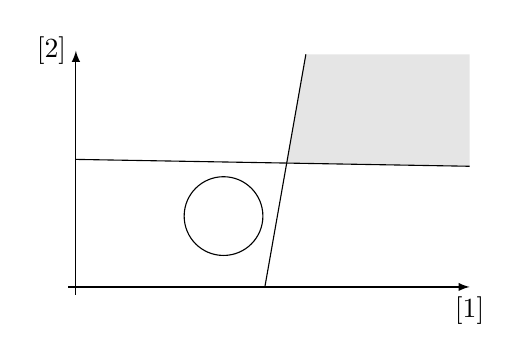
\begin{tikzpicture}
      \def\height{3}
      \def\length{5}
      \node at (0,0) {} coordinate (p0)  ++(0:\length*2.4/5) coordinate (p1) ;
      \node at (0,0) {} ++(90:\height*2.7/5) coordinate (p2) ;

      \draw[black] (p2) ++(-1:5) coordinate (p3);
      \draw[black] (p1) ++(80:3) coordinate (p4);
      \coordinate (p6) at (p3|-p4);

      \coordinate (p5) at (intersection cs:first line={(p2)--(p3)}, second line={(p1)--(p4)});
      \path[fill=gray!20] (p6) -- (p4) -- (p5) -- (p3);
      \draw[black] (p2) -- (p3);
      \draw[black] (p1) -- (p4);

      \draw[-latex] (0,-.1) - - (0,\height) node[left]{$\elem[2]{\thetai}$};
      \draw[-latex] (-.1,0) - - (\length,0) node[below]{$\elem[1]{\thetai}$};

      \node[draw,circle,minimum width=1cm] at (\length*.375,\height*0.3) {$\thetairestricted$};
    \end{tikzpicture}
    \caption{Boule $\set{B}(\thetairestricted,r)$.}\label{fig:ball_around_theta_restricted_fr}
  \end{subfigure}
  \hfill
  \begin{subfigure}{0.4\textwidth}
    \centering
    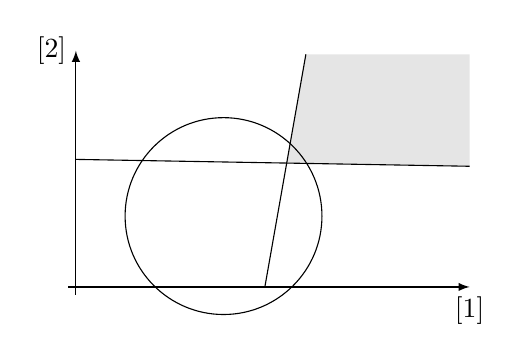
\begin{tikzpicture}
      \def\height{3}
      \def\length{5}
      \node at (0,0) {} coordinate (p0)  ++(0:\length*2.4/5) coordinate (p1) ;
      \node at (0,0) {} ++(90:\height*2.7/5) coordinate (p2) ;

      \draw[black] (p2) ++(-1:5) coordinate (p3);
      \draw[black] (p1) ++(80:3) coordinate (p4);
      \coordinate (p6) at (p3|-p4);

      \coordinate (p5) at (intersection cs:first line={(p2)--(p3)}, second line={(p1)--(p4)});
      \path[fill=gray!20] (p6) -- (p4) -- (p5) -- (p3);
      \draw[black] (p2) -- (p3);
      \draw[black] (p1) -- (p4);

      \draw[-latex] (0,-.1) - - (0,\height) node[left]{$\elem[2]{\thetai}$};
      \draw[-latex] (-.1,0) - - (\length,0) node[below]{$\elem[1]{\thetai}$};

      \node[draw,circle,minimum width=2.5cm] at (\length*.375,\height*0.3) {$\thetairestricted$};
    \end{tikzpicture}
    \caption{Boule $\set{B}(\thetairestricted,r)$ qui traverse les zones.}\label{fig:ball_around_theta_restricted_traversing_fr}
  \end{subfigure}
  \caption{Effets de la génération avec différent rayons $r$.}
\end{figure}

Alors, pour l'estimation on a besoin d'une méthode que puisse estimer $\Plinineq$ malgré le choix du rayon.
Une méthode qui puisse aussi classifier les zones (vue en \S\ref{sec:cons-about-mult_fr}).

\subsection{Détection}\label{sec:detection_ineq_fr}

Comme vu en~\eqref{eq:lambdafuntheta_fr}, les parties affines $\Plinineq[i][n]$ sont invariantes avec le temps.
Alors, si on estime $\Plinineqtildeestimate[i][n]$, on peut détecter l'attaques si il y a une différence entre la valeur estimée et la nominal $\Plinineqnominal[i][n]$.
On peut comparer pour n'importe quel mode non creux\footnote{$2^{Nc}$-zones sont completèment creuses et ne changent pas avec la triche (\S\ref{sec:impact-local-problem_fr}).}.
Par contre, comme on aura besoin de $\Plinineqtildeestimate$ pour la mitigation, on peut l'utiliser pour la détection aussi.

En fixant une borne $\epsilon_{\Plinineq}$, et en calculant une érreur
\begin{equation}
  E_{i}^{(0)}[k] =\norm{\Plinineqtildeestimate-\Plinineqnominal}_{F},
\end{equation}
avec une fonction de détection associée $\mathfrak{d}_{i}^{(0)}$:
\begin{equation}
  \label{eq:detection_ineq}
  \mathfrak{d}_{i}^{(0)}=\indicator{E_{i}^{(0)}[k]\geq\epsilon_{\Plinineq}},
\end{equation}
on détecte un attaque une fois que la borne soit surpassée, i.e., $\mathfrak{d}_{i}^{(0)}=1$.

\subsection{Estimation de paramètres multiples}\label{sec:cons-about-mult_fr}

On utilise une méthode de la \emph{famille de partitions}\footnote{Les méthodes dans cette famille résolvent des problèmes de régression et classification successifs.}
La méthode choisie est l'\EM{}~\cite{DempsterEtAl1977,Bishop2006}.

\subsubsection{Expectation Maximization}
Son objectif est de trouver, à partir de un jeux de données observables $\set{B}$, des estimateurs des paramètres $\set{P}$ qui maximisent le log de la vraisemblance marginal ${\ln\probability{\set{B};\set{P}}}$.
Les modèles normalement on des variables latentes (pas observables) dans un ensemble $\set{U}$.

Ce problème de maximiser ${\ln\probability{\set{B};\set{P}}}$ n'a pas de solution analytique.

À la place on maximise la valeur espérée du log de la vraisemblance de données complète $\ln\probability{\set{B},\set{U};\set{P}}$ par rapport les probabilités à posterior ${\probability{\set{U}|\set{B};\set{P}}}$.

Pour calculer les probabilités à posteriori on utilise d'estimations currantes $\set{P}$ dénotés $\set{P}_{\mathrm{cur}}$.

L'algorithm est résumé en Algorithm~\ref{alg:em_fr}.

\SetKwBlock{Estepfr}{ Pas E:}{}
\SetKwBlock{Mstepfr}{ Pas M:}{}
\begin{algorithm2e}[h]
  \DontPrintSemicolon%
  Initialiser $\set{P}_{\mathrm{new}}$\;
  \Repeat{$\set{P}_{\mathrm{cur}}$ a convergé}{
    $\set{P}_{\mathrm{cur}}\gets\set{P}_{\mathrm{new}}$\;
    \Estepfr{
      Calculer ${\probability{\set{U}|\set{B};\set{P}_{\mathrm{cur}}}}$\;
    }
    \Mstepfr{
      Estimer $\set{P}_{\text{new}}$: \begin{equation}
        \label{eq:m_step_fr}
        \set{P}_{\mathrm{new}}=\argmax_{\set{P}}\ \expectation[{\probability{\set{U}|\set{B};\set{P}_{\mathrm{cur}}}}]{\ln\probability{\set{B},\set{U};\set{P}}}
      \end{equation}
    }
}
 \caption{Expectation Maximization}\label{alg:em_fr}
\end{algorithm2e}

\subsection{Adaptation pour le problème étudié}
Comme \EM{} est probabilistique on doit incorporer un comportement probabilistique dans notre modèle~\eqref{eq:lambdafuntheta_fr}.

On enlève les indices $i$ et $[k]$, pour faciliter la lecture.

D'abord, on utilise les homolques stochastiques $\random{\thetai}$ and $\random{\lambdai}$.
Si on surveille $O$ échanges entre agent et coordinateur, on voit variables d'entrée et réponses, ${\random{\vec{\theta}}_{o}}$ et ${\random{\vec{\lambda}}_{o}}$, ${o\in\set{O}=\{0\until O-1\}}$.
On les organise en ${\random{\Theta},\random{\Lambda}\in\R^{c\times O}}$.
Et la tuple ${(\random{\Theta},\random{\Lambda})}$ est l'ensemble observable $\set{B}$.

Comme chaque $\randomvec{\theta}_{o}$ reste dans une région, on l'associe à une variable ${z\in\set{Z}=\{0\until Z-1\}}$ qui indique le numéro de zone.
Notre modèle devient

\begin{equation}\label{eq:linear_cheating_random_fr}
  \randomvec{\lambda}_{o}=
  \begin{cases}
    -\tilde{P}^{0}\randomvec{\theta}_{o}-\tilde{\vec{s}}^{0},&\text{si dans zone } 0\\
    \qquad\quad \vdots&\qquad\quad \vdots\\
    -\tilde{P}^{Z-1}\randomvec{\theta}_{o}-\tilde{\vec{s}}^{Z},&\text{si dans zone } {Z-1}\\
  \end{cases}.
\end{equation}

En~\cite{FariaSoromenho2010}, une méthode similaire est appellée \emph{mixture de régressions linéaires}, mais comme on a des fonctions \pwa{}, on l'apelle \emph{mixture de régressions affines}.

Comme on ne connait pas l'appartenance de chaque point observé, associe l'index $z$ de chaque observation ${(\randomvec{\lambda}_{o}, \randomvec{\theta}_{o})}$ à une variable latente ${\random{z}_{o}}$.
On organise $\random{z}_{o}$ en ${\random{Z}\in\R^{1\times O}}$, qui est notre ensemble pas observable $\set{U}$.

On suppose que $\random{z}_{o}$ suit une distribution catégorique, avec des probabilités associées ${\Pi=\{\pi^{z}|z\in\set{Z}\}}$ tels que
\[\probability{\random{z}_{o}=z}=\pi^{z} \in [0,1], \qquad \sum_{z\in\set{Z}} \pi^{z} = 1.
\]

On construit l'ensemble de paramètres ${\set{P}=\setbuild{\set{P}^{z}}{z\in\set{Z}}}$, avec ${\set{P}^{z}=(\tilde{P}^{z},\tilde{\vec{s}}^{z},\pi^{z})}$.

\begin{remark}
  On estime $\pi^{z}$ et $\tilde{\vec{s}}^{z}$ puremen pour mettre le modèle à jour et contraindre l'identification de $\tilde{P}^{z}$.
\end{remark}

Pour $\vec{\theta}$, on considère une densité de probabilité impropre et non informative~\cite{ChristensenEtAl2010}
\[
  \probability{\randomvec{\theta}_{o}} \,\propto \,1,
\]
que signifie qu'on connait presque sûrement la valeur de $\randomvec{\theta}_{o}$.

Une fois définies les variables d'entrées et latents, on modèle la réponse $\random{\lambda}_{o}$ comme une variable normale multivariables avec fonction de densité de probabilité
\begin{equation}
  \label{eq:multivariate_gaussian_fr}
\probability{\randomvec{\lambda}_{o}|\randomvec{\theta}_{o},\random{z}_{o}=z; \set{P}^{z}} = \mathcal{N}(\randomvec{\lambda}_{o};f(\randomvec{\theta}_{o};\set{P}^{z}),{\Sigma^{z}}),
\end{equation}
qui suivant le modèle de la mixture de régressions affines~\eqref{eq:linear_cheating_random_fr} a comme valeur espérée
\begin{equation}
  f(\randomvec{\theta}_{o};(P,\vec{s},\pi))=-{P}\randomvec{\theta}_{o}-{\vec{s}},
\end{equation}

Les matrices de covariance $\Sigma^{z}$ tend à $0_{c}$, s'approachant des valeurs originales des fonctions en~\eqref{eq:lambdafuntheta_fr}.

Un exemple de la répresentation de tel fonction pour $1$ dimension est vue en Fig.~\ref{fig:affine_gaussian_mixture}, où points plus sombres présentent plus de probabilité que les plus clairs.
\begin{figure}[h]
  \centering
  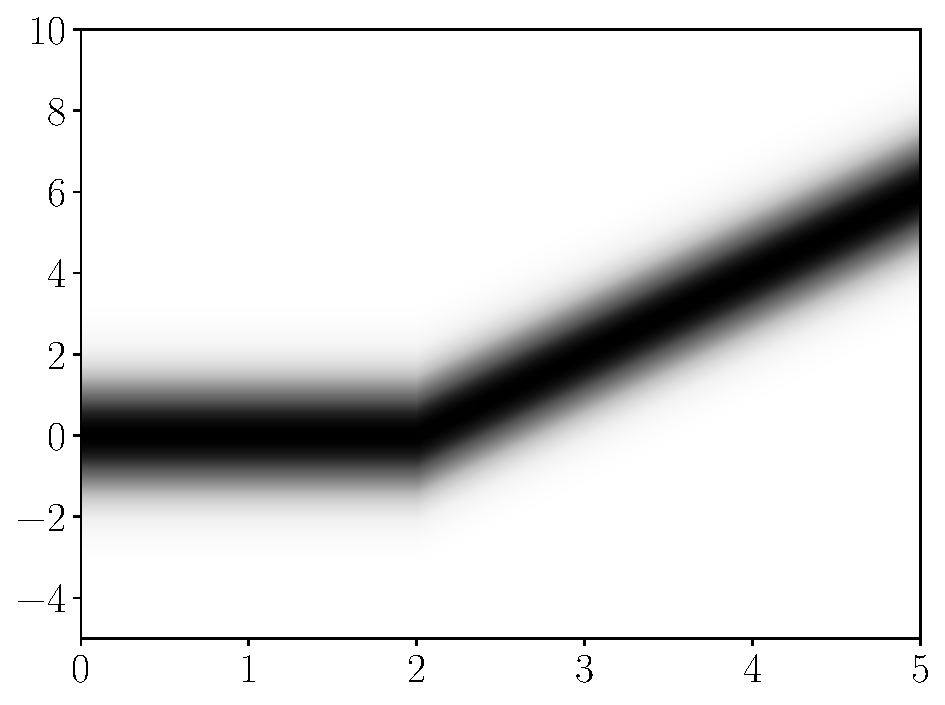
\includegraphics[width=0.7\textwidth]{../img/resilient_ineq/pwa.pdf}
  \caption{Mixture gaussianne pour \pwa{} d'une dimension.}\label{fig:affine_gaussian_mixture_fr}
\end{figure}

Les probabilités à posteriori $\zeta_{zo}(\set{P})=\probability{\random{z}_{o}=z|\randomvec{\lambda}_{o},\randomvec{\theta}_{o};\set{P}}$, aussi appellées \emph{responsabilités}, sont calculées:
\begin{align}
  \label{eq:responsibilities_fr}
\zeta_{zo}(\set{P})&=\frac{\pi_{z}{\mathcal{N}(\randomvec{\lambda}_{o};f(\randomvec{\theta}_{o};\set{P}^{z}),{\Sigma^{z}})}}{\sum\limits_{j=1}^{Z}\pi_{j}\mathcal{N}(\randomvec{\lambda}_{o};f(\randomvec{\theta}_{o};\set{P}^{j}),{\Sigma^{j}})}.
\end{align}
On les appelle responsabilités car on calcule la probabilité de que la zone $z$ soit responsable d'avoir généré l'observation $o$.

On calcule la valeur espérée de ${\ln\probability{\random{\Theta},\random{\Lambda},\random{Z};\set{P}}}$ par rapport à ${\zeta_{zo}(\set{P}_{\mathrm{cur}})}$~\cite[Chapitre 9]{Bishop2006} en utilisant
\begin{align}
  \label{eq:completedataLogLikelihood_expectation}
\expectation[{\zeta_{zo}(\set{P}_{\mathrm{cur}})}]{\ln\probability{\random{\Theta},\random{\Lambda},\random{Z};\set{P}}}&= \sum_{o\in\set{O}}\sum_{z\in\set{Z}}  \zeta_{zo}(\set{P}_{\mathrm{cur}})\alpha_{zo},
\end{align}
où ${\alpha_{zo}=\ln{\pi_{z}}+\ln{\mathcal{N}(\randomvec{\lambda}_{o};f(\randomvec{\theta}_{o};\set{P}^{z}),{\Sigma^{z}})}}$.

Pour faciliter les calculs, on introduit une variable $\vec{\phi}^{z}$ pour intégrer les paramètres, ainsi comme on a fait dans le cas avec le cas \RLS{} (\S\ref{sec:about-estimation_fr})
\begin{equation}
  \vec{\phi}^{z}=\left[
      \begin{matrix}
      \vectorize{\tilde{P}^{z}}^{T}\\\tilde{\vec{s}}^{z}
      \end{matrix}
    \right].
\end{equation}

Pour trouver le $\vec{\phi}^{z}$ optimal pour le problème en~\eqref{eq:m_step_fr}, on prend les gradients de~\eqref{eq:completedataLogLikelihood_expectation_fr} par rapport aux vecteurs $\vec{\phi}^{z}$ et on les fait disparaître.

On trouve comme solution
\begin{equation}
  \label{eq:mstepestimation_fr}
  \vec{\phi}^{z}_{\mathrm{new}}=\pseudoinv{(\Xi^{z}\random{\Omega})}\Xi^{z}\vectorize{\random{\Lambda}},
\end{equation}
où
${\random{\Omega}=[\hadamard{(\Upsilon \random{\Theta}\Delta)}{Y};G]}$,
avec des matrices
${\Upsilon=\kron{\1_{c}^{T}}{I_{c}}}$,
${\Delta=\kron{I_{O}}{\1_{c}^{T}}}$,
${Y=\kron{G}{\1_{c}}}$,
${G=\kron{\1_{O}^{T}}{I_{c}}}$,
et
\[{\Xi^{z}={\diag(\sqrt{{\zeta(z_{z1};\set{P}_{\mathrm{cur}})}}I_{c},\cdots,\sqrt{{\zeta(z_{zO};\set{P}_{\mathrm{cur}})}}I_{c})}}.\]
Si on fait le même, mais pour $\pi^{z}$ on trouve
\begin{equation*}
  \label{eq:3_fr}
  \pi^{z}=\sum\limits_{o\in\set{O}}\tfrac{\zeta_{zo}(\set{P}_{\mathrm{cur}})}{O}.
\end{equation*}

On voit que~\eqref{eq:mstepestimation_fr} est une solution pondéré d'un \LS{}, avec les responsabilités comme poids,  qui ajustent la contribution de tous les observations aux modèles de régression.

Il existe quelques similarités avec la méthode K-planes (et k-means) (voir~\cite{BradleyMangasarian2000}), mais l'\EM{} est plus transigen.
Au lieu d'affecter l'observation à un zone avec 100\% de sûreté, \EM{} utilise la responsabilité de chase zone (\emph{affectation fluide}).

Quand $\vec{\phi}_{z}^{\mathrm{new}}$ converge, on peut récupérer les estimations de $\tilde{P}^{z}$ et $\tilde{\vec{s}}^{z}$, pour utiliser dans les schémas de détection et mitigation.

Comme les indices $z$ ne correspondent pas forcément à ceux de~\eqref{eq:lambdafuntheta_fr}, il faut trouver le $z$ qui correspond à la $0$-zone.
On prend l'observation $o$ qui correspond à $\thetairestricted$, qui comme on sait appartient à la $0$-zone, et trouve la région plus probable avec
\begin{equation*}\label{eq:argmaxz_fr}
  \arg\underset{z}{\max\!.}\ {\zeta_{zo}(\set{P})}.
\end{equation*}

Le paramètre avec cet index correspond à notre $\Plinineqtildeestimate$.

\subsubsection{Quelques réserves}

C'est connu~\cite{CeleuxGovaert1992,Bishop2006,BaudryCeleux2015} que l'algorithme peut présenter une convergence lente.
En~\cite{FariaSoromenho2010}, les autrices comparent la convergence de l'\EM{} avec quelques variantes (\sEM{} et \CEM{}).

Un autre point est la dépendance de la solution par rapport l'initialisation de l'algorithme~\cite{KarlisXekalaki2003,BaudryCeleux2015}.

Encore un autre et l'inversion de quelques variables (notably the covariance $\Sigma$) quand utilisant modèles de dimensions élevés.
Ça va dépendre des observations $O$ et le nombre de zones $Z$.
Une façon de contrer l'éffet est inclure dans les éléments estimés.
Une autre solution est considérer la matrice diagonal avec les mêmes valeurs~\cite{KarlisXekalaki2003}.
Encore autre solution est d'utiliser la technique appellée \emph{recuite simulée}~\cite{CeleuxGovaert1992,OzerovFevotte2010}, où les covariances sont initialisées avec des valeurs importantes, indiquant l'incertitude des paramètres, et les faires decroitre à chaque itération.
Dans ce travail on a utilisé les deux dernières solutions combinées.

\end{document}
